\documentclass[review,3p,10pt,sort&compress]{elsarticle}
%\documentclass[preprint,5p,10pt,sort&compress]{elsarticle}

\usepackage{amsfonts,amsmath,amssymb,graphicx,dsfont,color,multirow,epstopdf}
\usepackage[tight,normalsize,sf,sf]{subfigure}
%\usepackage{amstext,mathptmx,float,booktabs,bbm}

\journal{Signal Processing}
\linespread{1.25}

\begin{document}

\begin{frontmatter}

\title {Improved PPVO-based high-fidelity reversible data hiding}

\author{Haorui Wu}
\ead{hrwu@bjtu.edu.cn}

\author{Xiaolong Li}
\ead{lixl@bjtu.edu.cn}

\author{Yao Zhao\corref{cor}}
\cortext[cor]{Corresponding author. Tel./Fax:  +86 10 51688667.}
\ead{yzhao@bjtu.edu.cn}

\author{Rongrong Ni}
\ead{rrni@bjtu.edu.cn}

\address[mymainaddress]{Institute of Information Science, Beijing Jiaotong University, Beijing 100044, China}
\address[mysecondaryaddress]{Beijing Key Laboratory of Advanced Information Science and Network Technology, Beijing 100044, China}

\begin{abstract}
%Pixel-value-ordering (PVO) based reversible data hiding (RDH) is widely studied in recent years.
Most pixel-value-ordering (PVO) based reversible data hiding (RDH) methods conduct pixel prediction on image blocks, while a recently proposed pixel-based PVO (PPVO) method changes the blockwise prediction to pixelwise manner and achieves better embedding performance. However, in PPVO, the prediction result is not accurate since some pixels close to the to-be-predicted one are not utilized for prediction. Moreover, pixels with different complexity are not fully exploited and the embedding performance of PPVO is not optimized. Then, to better determine pixel context for prediction as well as make full use of image local correlation, an improved PPVO-based RDH method is proposed in this paper. First, to improve the prediction accuracy, a new prediction strategy is proposed in which the pixel context is properly selected. Then, a new embedding strategy is proposed for performance optimization based on multiple histograms generation and modification with multi-sized prediction contexts. Experimental results verify that the proposed method is superior to PPVO and some other PVO-based RDH methods.

\end{abstract}


\begin{keyword}
   Reversible data hiding \sep pixel-value-ordering \sep pixelwise prediction \sep multiple histograms generation and modification
\end{keyword}

\end{frontmatter}

%----------------------------------------------------------------------------------------
\section{Introduction}\label{sec:1}
% RDH PEH PVO MHM
%In recent days, the tampering and propagation of multimedia data have been getting more and more convenient.

Information hiding has received extensive attention nowadays \cite{IJcox,Fridrich}. Among existing information hiding approaches, reversible data hiding (RDH) can exactly extract the embedded data and losslessly recover the cover image as well, which is useful for the information hiding of sensitive images \cite{shi}.

Up to now, many RDH methods have been proposed, such as difference expansion (DE) \cite{
Tian2003DE,
Qin2013An,
Thodi2007Expansion,
Hu2009DE,
Li2013A},
histogram shifting (HS) \cite{
Hong2009Reversible,
Hong2010A,
Xiaolong2013General,
Wang2018A},
prediction-error expansion (PEE) \cite{
Sachnev2009Reversible,
Tsai2009Reversible,
Gao2011Lossless,
Li2011Efficient,
Hong2011Adaptive,
Wu2012Reversible,
Qin2013An,
Ou2013Pairwise,
Dragoi2014Local,
Li2015Efficient,
Dragoi2016Adaptive,
Wang2017Rate}
and so on. 
The first DE-based method is proposed by Tian \cite{Tian2003DE}. By DE, the pixel difference is expanded for reversible embedding. 
For HS-based RDH, it is first proposed by Ni \emph{et al}. \cite{hs1}, and the data embedding is conducted by modifying the image intensity histogram. 
Later on, the technique prediction-error expansion (PEE) is proposed by Thodi and Rodriguez \cite{Thodi2007Expansion}, in which the image pixels are first predicted and then the resulting prediction-errors are expanded or shifted for reversible embedding. Compared with DE and HS, PEE is the most effective RDH approach nowadays due to its fine balance between the embedding capacity and distortion.
After that, many improvements for PEE focusing on pixel prediction and prediction-error histogram (PEH) modification are proposed, e.g., accurate predictor design \cite{Thodi2007Expansion,Fallahpour2008Reversible,Hu2009DE,Hong2009Reversible,Sachnev2009Reversible,Ioan2014Local,Ioan2015On}, adaptive histogram modification \cite{}, high dimensional histogram modification \cite{Ou2013Pairwise,Li2013A,Dragoi2016Adaptive}, and multiple histograms modification \cite{Li2015Efficient,Xiang2015A,Bo2016Improved}, etc.

Recently, a novel improvement of PEE taking pixel-value-ordering (PVO) to provide accurate prediction has been proposed \cite{
Li2013PVO,
Peng2014IPVO,
Ou2014PVOk,
Qu2015PPVO,
Xiang2015A,
Bo2016Improved,
Weng2016Reversible,
Weng2017Optimal,
He2018Reversible,
Kim2018Skewed}.
% PVO
The original PVO-based method is proposed by Li \emph{et al.} \cite{Li2013PVO}. In this method, the cover image is first divided into equal-sized non-overlapping blocks and the secret data is embedded into the largest/smallest pixel of each block via modifying its prediction-errors.
% IPVO PVO-k
After that, Peng \emph{et al.} proposed an improved PVO-based method in \cite{Peng2014IPVO} by utilizing more smooth blocks for reversible embedding. In \cite{Ou2014PVOk}, Ou \emph{et al.} proposed another PVO-based method called PVO-$k$ which modifies the first $k$ largest/smallest pixel values in each block for performance enhancement.
% Ou He pairwise
Later on, Ou \emph{et al.} \cite{Bo2016Improved} and He \emph{et al.} \cite{He2018Reversible} proposed a way to better explore the pixel relations in each block for PVO. In these methods, two prediction-errors in a block are paired together to generate a two-dimensional PEH and proper histogram modification manners are designed for reversible embedding.
% wang weng ,multi-block-size
Besides, Wang \emph{et al.} \cite{Xiang2015A} and Weng \emph{et al.} \cite{Weng2016Reversible} proposed to dynamically determine the block size to better use pixels in smooth regions.
% PPVO
Moreover, unlike the blockwise prediction used in previous PVO-based methods, Qu \emph{et al.} proposed the so-called pixel-based PVO (PPVO) in \cite{Qu2015PPVO} by utilizing pixelwise prediction. In this method, each pixel is predicted by the largest/smallest pixel value of its context, and high embedding capacity is achieved.
% Kim
%Recently, Kim \emph{et al.} propose a novel RDH scheme \cite{Kim2018Skewed} with a more accurate full-enclosing predictor. A skewed two prediction-error histograms are generated and only the short tails are used to embed data to reduce shifting distortion.
PPVO is an effective improvement of PVO, and it is experimentally verified better than some PVO-based RDH methods with both higher embedding capacity and better marked image quality.
However, for the prediction in PPVO, some pixels close to the to-be-predicted one are not involved so that the prediction is not accurate. This drawback limits its embedding performance. On the other hand, since all pixels are predicted with identical context without considering the different local complexity, the embedding performance of PPVO is not optimized.

In this paper, based on the above considerations, a novel RDH method is proposed to improve PPVO \cite{Qu2015PPVO}. Unlike PPVO, some pixels close to the to-be-predicted one are taken as a part of context for prediction, contributing to the prediction accuracy enhancement. In this way, shaper PEH can be generated which is more suitable for reversible embedding. Moreover, to better exploit image redundancy and for performance optimization of PPVO, a new embedding strategy is proposed by conducting multiple histograms generation and modification with multi-sized prediction contexts. By this strategy, pixels with different local complexity are predicted by different sized context. Then, multiple PEHs are generated according to the employed different pixel context and then modified for data embedding. Experimental results verify that the proposed method outperforms PPVO \cite{Qu2015PPVO}, and it is superior to some other PVO-based RDH methods \cite{Peng2014IPVO,Ou2014PVOk} as well.


The rest of the paper is organized as follows. Section \ref{sec:2} presents a brief review of PPVO \cite{Qu2015PPVO}. The details of the proposed method improving the original PPVO is introduced in Section \ref{sec:3}. Then, the experimental results are given in Section \ref{sec:4}. Finally, Section \ref{sec:5} concludes the paper.

%----------------------------------------------------------------------------------------
\section{Related Work}\label{sec:2}
In this section, as a prior knowledge, the PPVO method of Qu \emph{et al.} \cite{Qu2015PPVO} is briefly reviewed. Unlike the previous PVO-based methods such as \cite{Li2013PVO} and \cite{Peng2014IPVO}, PPVO conducts prediction in a pixelwise manner. Specific data embedding and extraction procedures are presented as follows.

%we will review the PPVO method of Qu \emph{et al.} \cite{Qu2015PPVO}. Classical PVO-based RDH methods, such as the original PVO-based method \cite{Li2013PVO} and the improved PVO-based method \cite{Peng2014IPVO}, usually divide the cover image into equal-sized non-overlapping blocks at the beginning. Then, in each block, only the largest and smallest pixels are utilized for embedding while others pixels are unchanged, leading to the insufficient use of smooth pixels. In order to make better use of the smooth pixels, Qu \emph{et al.} proposed the PPVO method \cite{Qu2015PPVO}, which conducts prediction in a pixel-wise manner.

\begin{figure*}
\centering
\subfigure[Context of $x$ with $n=15$.]{
    \begin{minipage}[t]{0.31\linewidth}
    \centering
    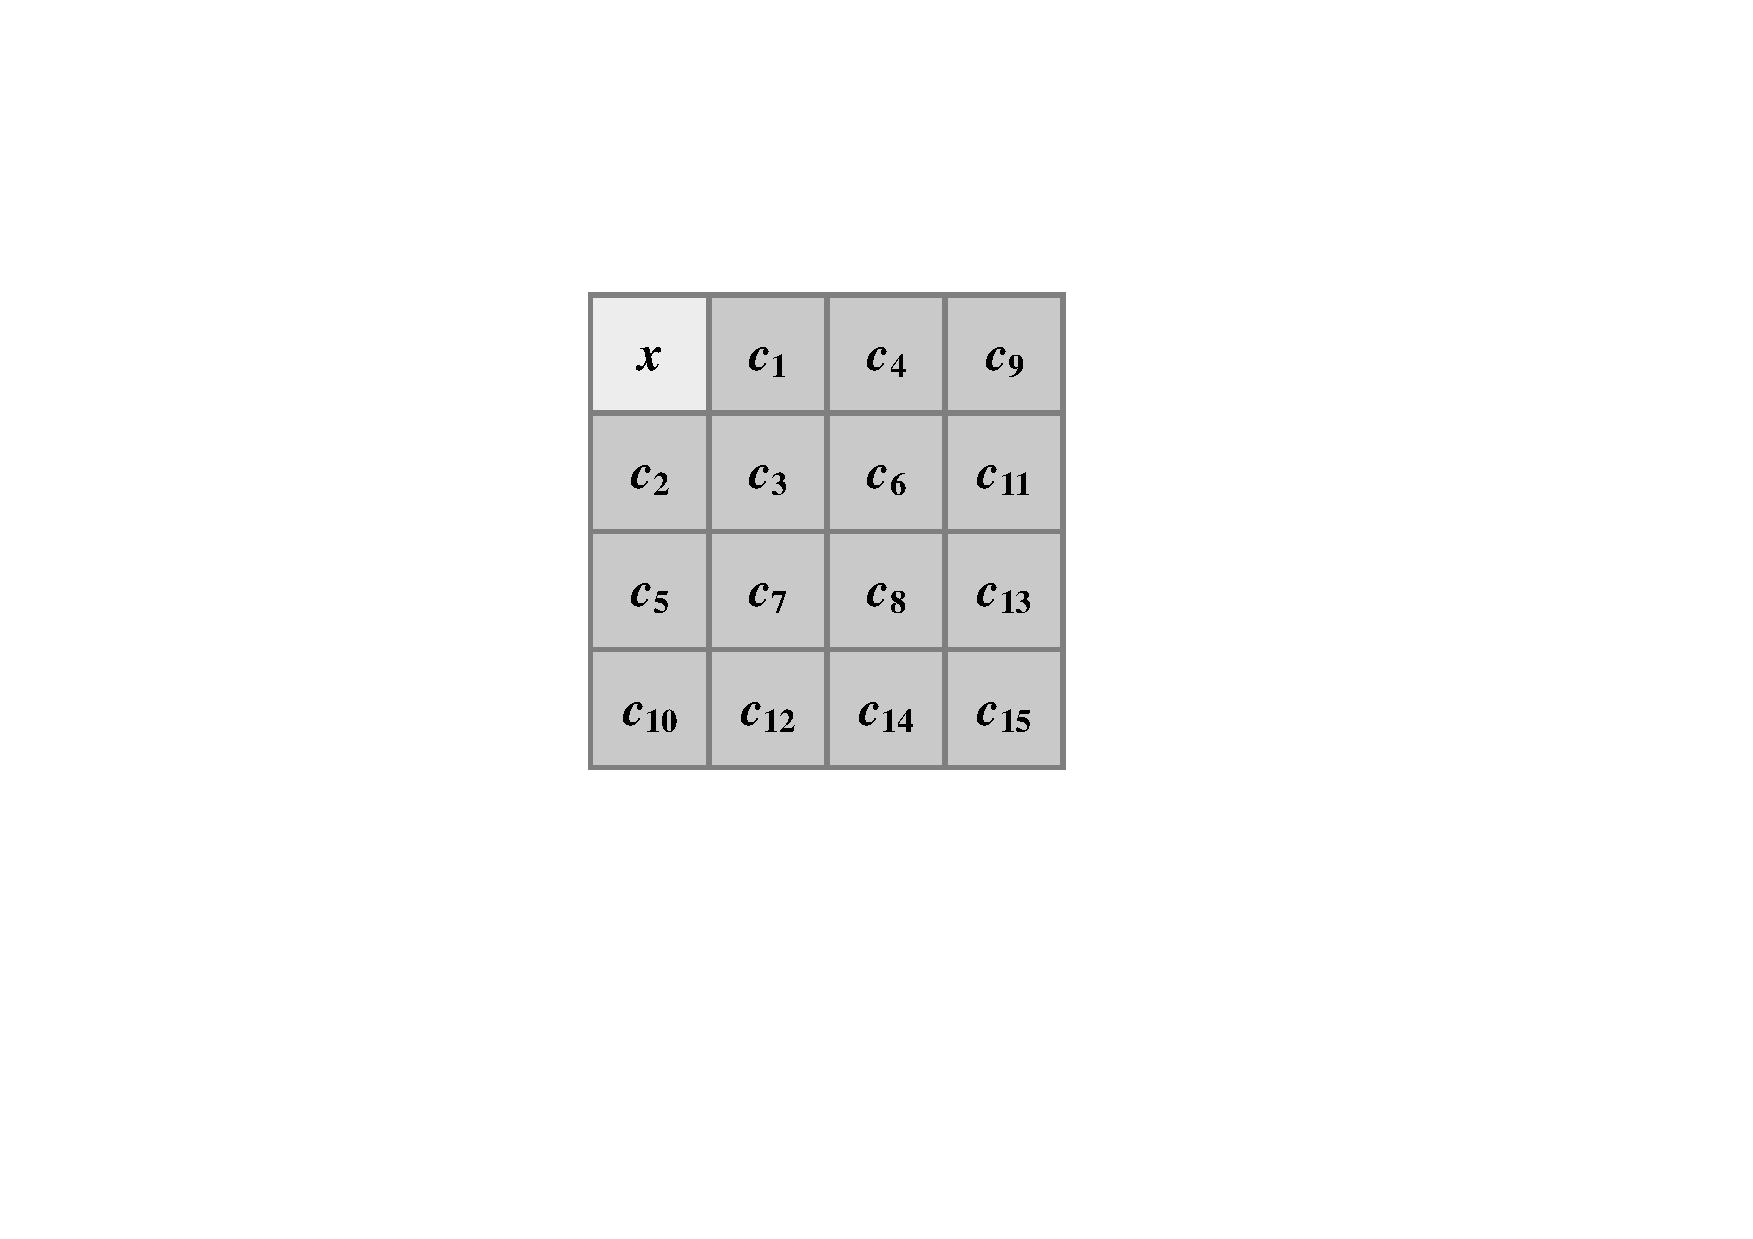
\includegraphics[width=0.75\textwidth]{figures/PPVOContext.pdf}
    \end{minipage}
}
\subfigure[PEH for $x \in S_1 \cup S_4$.]{
    \begin{minipage}[t]{0.31\linewidth}
    \centering
    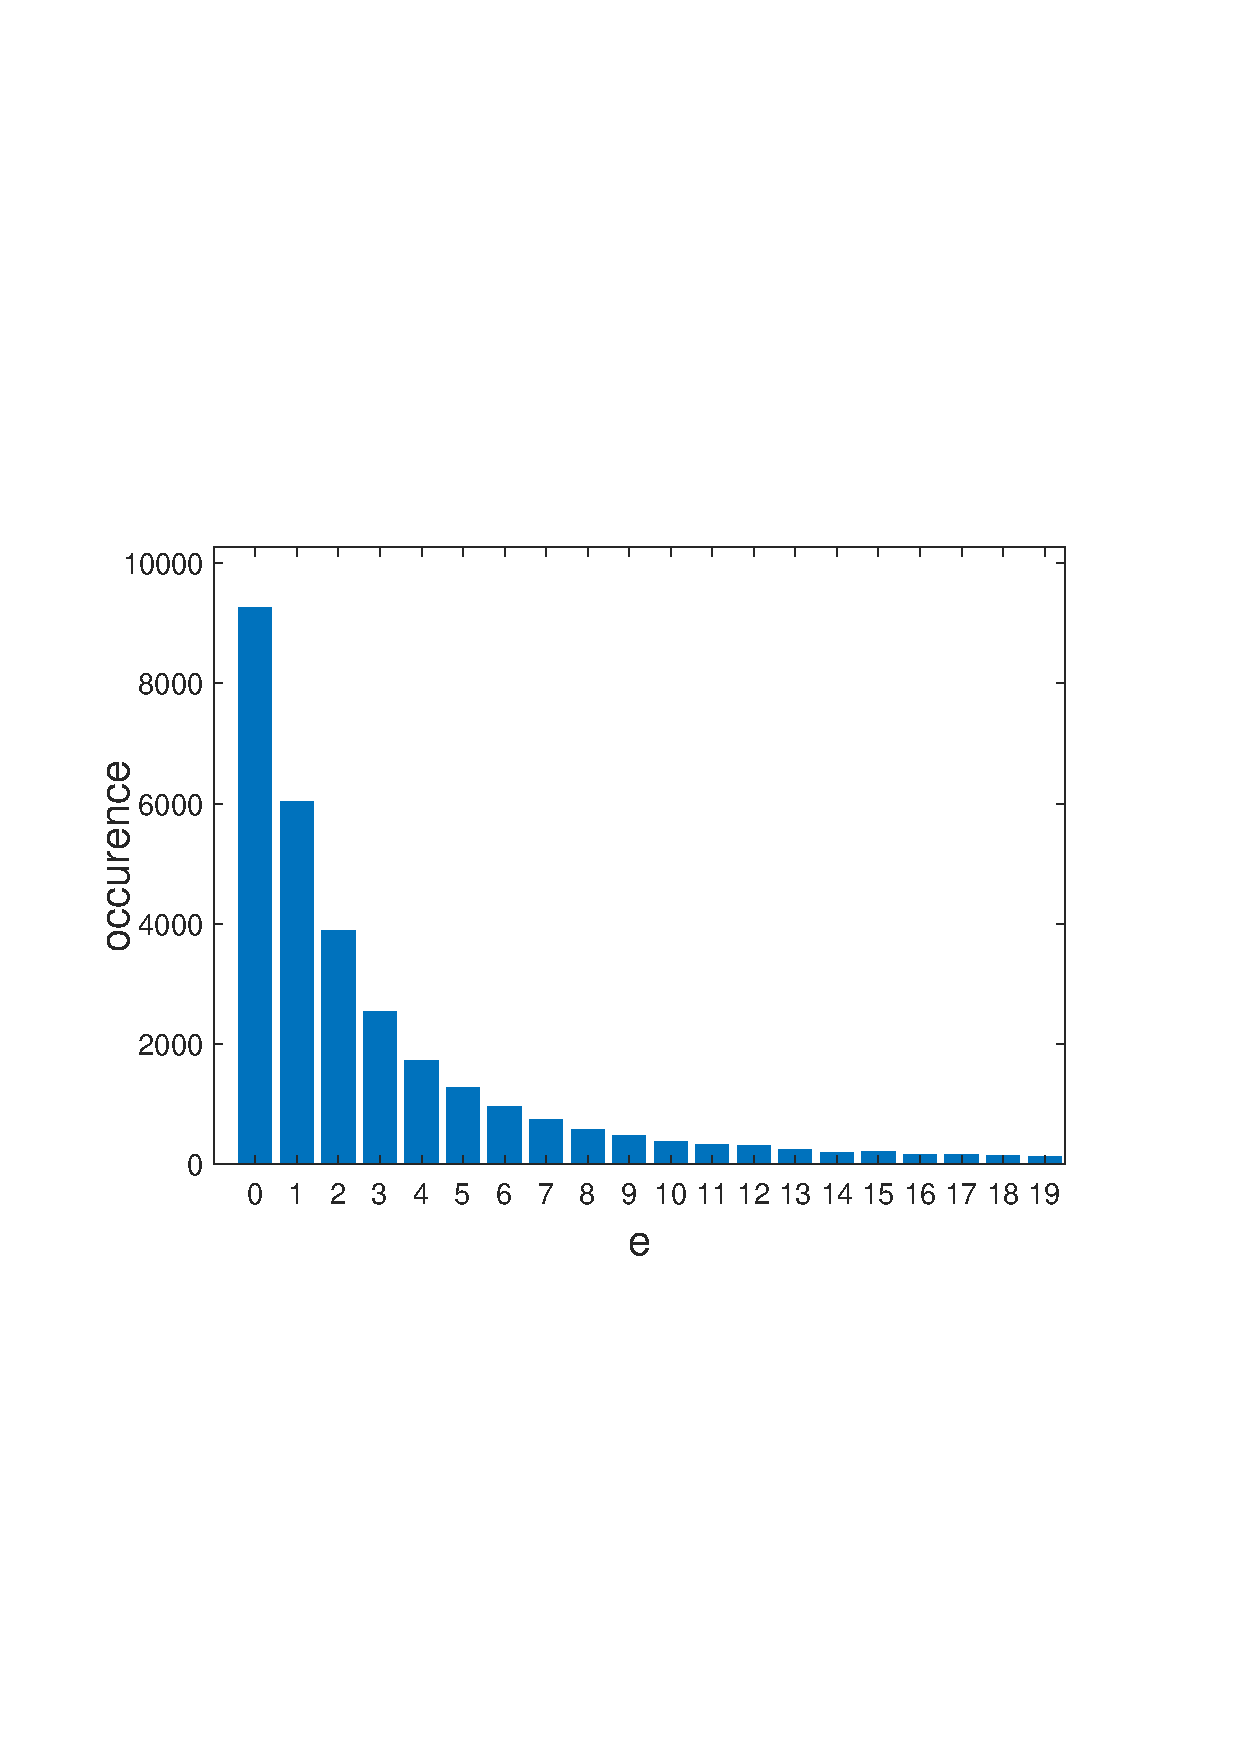
\includegraphics[width=1\textwidth]{figures/PPVOdmax.pdf}
    \end{minipage}
}
\subfigure[PEH for $x \in S_2 \cup S_3$.]{
    \begin{minipage}[t]{0.31\linewidth}
    \centering
    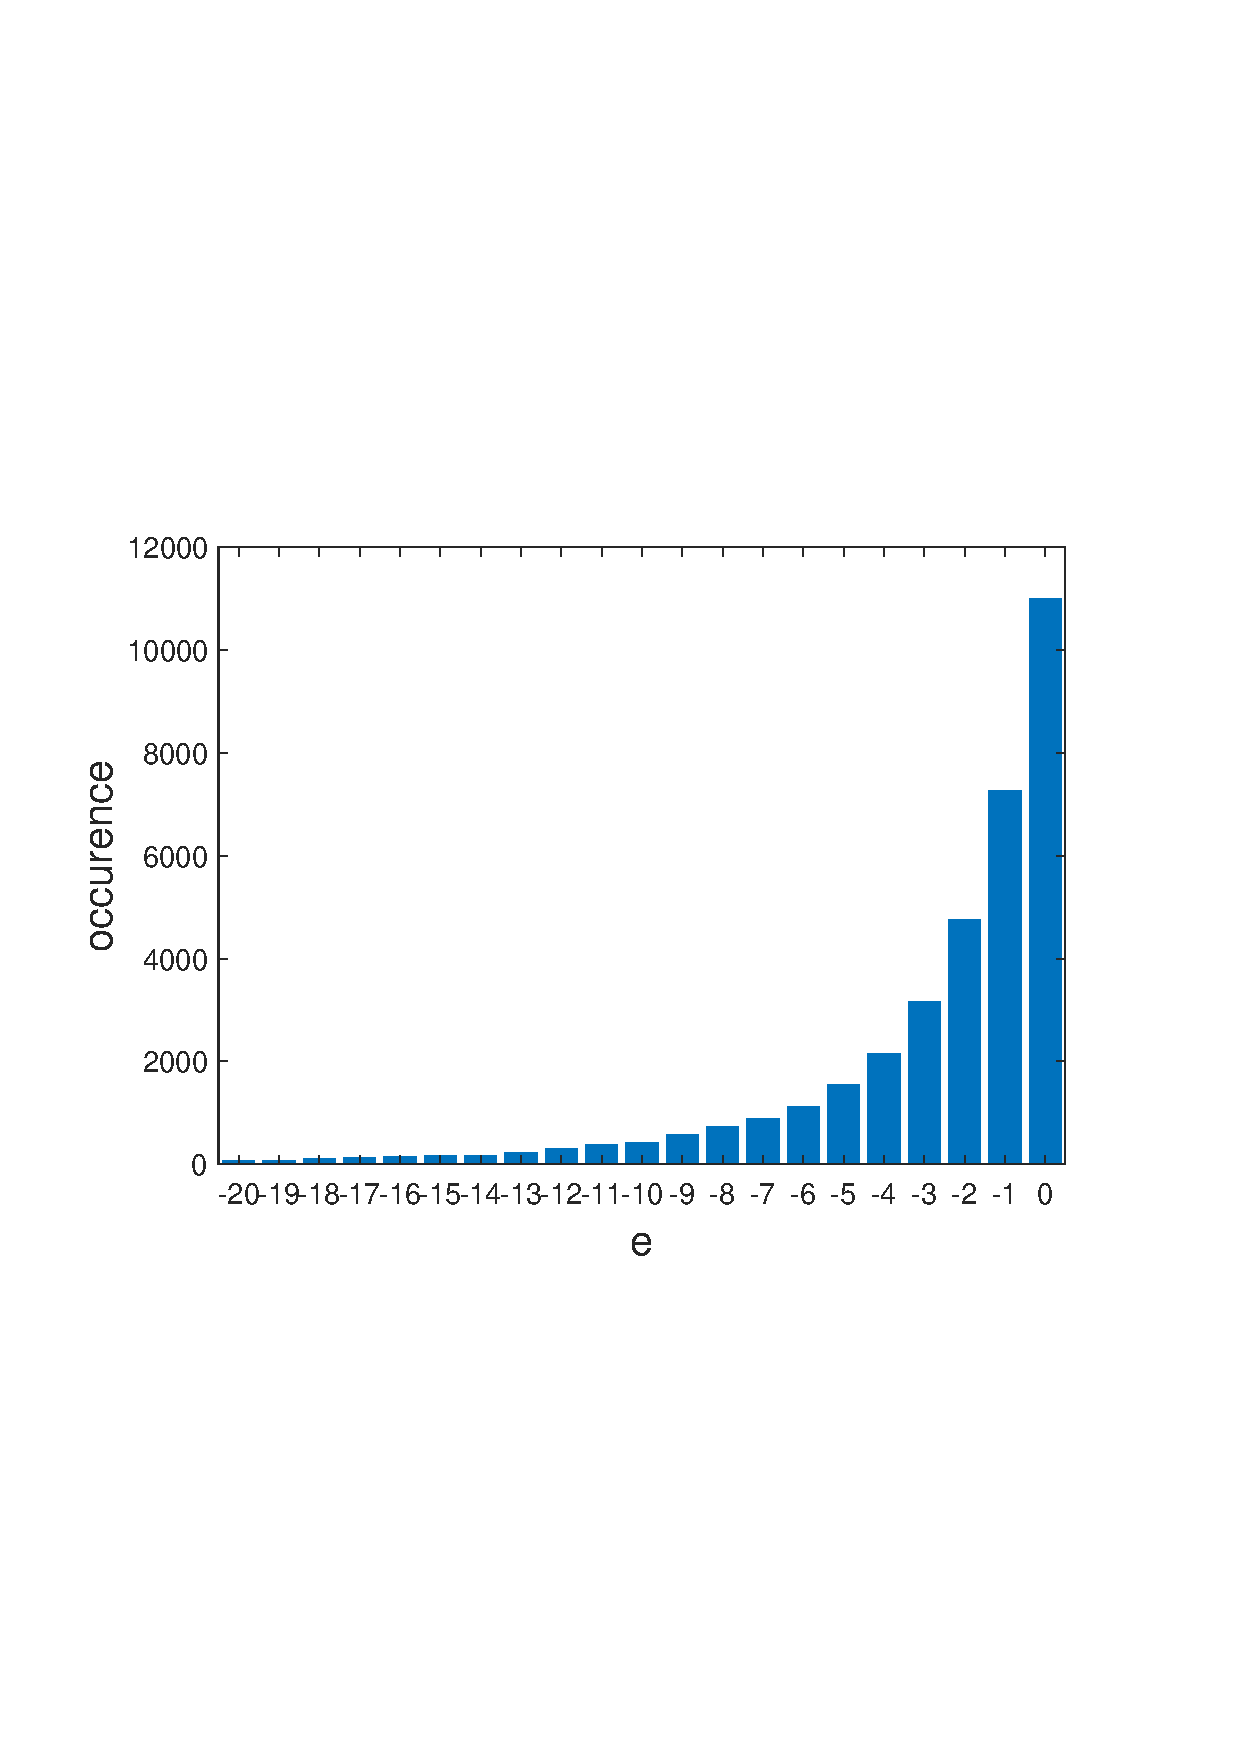
\includegraphics[width=1\textwidth]{figures/PPVOdmin.pdf}
    \end{minipage}
}	
\centering
\caption{Prediction context and the PEHs for the image Lena with pixels in $S_1 \cup S_4$ and $S_2 \cup S_3$, for PPVO \cite{Qu2015PPVO}.}
\label{Fig.PPVOCNandHist}
\end{figure*}

First of all, to avoid the overflow and underflow problem, pixels valued 0 are modified to 1 and pixels valued 255 are modified to 254. Then, for a target pixel $x$, its prediction context is defined by its neighboring pixels in the down right region, as shown in Fig. \ref{Fig.PPVOCNandHist}(a). More specifically, a prediction context $C=\{c_1,...,c_n\}$ is formed, where $n$ is the number of context pixels.
Next, sort the context pixels, and four cases may occur for the prediction of $x$. That is to say, cover pixels used for data embedding are grouped into four sets including
\begin{equation}\label{eq:S}
\begin{array}{ll}
    S_1 = \{ x | c_{\rm max} \neq c_{\rm min}, x \geq c_{\rm max} \} \\
    S_2 = \{ x | c_{\rm max} \neq c_{\rm min}, x \leq c_{\rm min} \} \\
    S_3 = \{ x | c_{\rm max}   =  c_{\rm min}, x \leq c_{\rm min}, c_{\rm min} \neq 254 \} \\
    S_4 = \{ x | c_{\rm max}   =  c_{\rm min}, x \geq c_{\rm max}, c_{\rm max} =  254 \} \\
\end{array}
\end{equation}
where $c_{\rm max}$ and $c_{\rm min}$ represent the largest and smallest pixel values in $C$, respectively, i.e., $c_{\rm max} =\max\{c_1,...,c_n\}$ and $c_{\rm min} =\min\{c_1,...,c_n\}$. Notice that, pixels outside the four sets are skipped and not utilized for embedding. In this way, $x$ is predicted as $\widehat{x}$ by
\begin{equation}\label{eq:xhat1}
    \widehat{x} = \left\{\begin{array}{ll}
    c_{\rm max},  & \text{if } x \in S_1 \cup S_4 \\
    c_{\rm min},  & \text{if } x \in S_2 \cup S_3
\end{array}\right.
.
\end{equation}
Then, the prediction-error is defined as $e = x - \widehat{x}$. Accordingly, $e \geq 0$ if $x \in S_1 \cup S_4$, and $e \leq 0$ if $x \in S_2 \cup S_3$. Here, the standard $512 \times 512$ sized gray-scale image Lena is taken for example, and the corresponding PEHs counting the frequency of $e$ are shown in Fig. \ref{Fig.PPVOCNandHist}(b) and (c), for pixels in $S_1 \cup S_4$ and $S_2 \cup S_3$, respectively. The highest frequency of both two PEHs locates at bin 0. Therefore, for each of the two PEHs, the bin 0 is expanded to embed data, and other bins are shifted to create vacancies. That is to say, the prediction-error $e$ is modified to $\widetilde{e}$ as follows for data embedding
\begin{equation}\label{eq:PPVOMPE}
    \widetilde{e} = \left\{\begin{array}{ll}
    e + b,  & \text{if } x \in S_1 \cup S_4 \text{ and } e = 0 \\
    e + 1,  & \text{if } x \in S_1 \cup S_4 \text{ and } e > 0 \\
    e - b,  & \text{if } x \in S_2 \cup S_3 \text{ and } e = 0 \\
    e - 1,  & \text{if } x \in S_2 \cup S_3 \text{ and } e < 0
\end{array}\right.
\end{equation}
where $b \in \{0,1\}$ is a data bit to be embedded. Finally, the marked pixel is determined as $\widetilde{x} = \widehat{x} + \widetilde{e}$.

The embedding process of PPVO for a cover image is performed in the raster-scan order and the extraction process is implemented in reverse order. Thus, the prediction context of each cover pixel and its corresponding marked pixel are the same. Moreover, in the embedding process, for $x \in S_1 \cup S_4$, it is either increased by 1 or unchanged, and for $x \in S_2 \cup S_3$, it is either decreased by 1 or unchanged, the marked pixel $\widetilde{x}$ can be classified into the same group as its cover $x$ according to \eqref{eq:S}. Then, the extraction and recovery process can be conducted as follows. First, a marked pixel $\widetilde{x}$ is predicted as
\begin{equation}\label{eq:xhat2}
    \widehat{x} = \left\{\begin{array}{ll}
    c_{\rm max},  & \text{if } \widetilde{x} \in S_1 \cup S_4 \\
    c_{\rm min},  & \text{if } \widetilde{x} \in S_2 \cup S_3
\end{array}\right.
.
\end{equation}
Then, the marked prediction-error is computed by $\widetilde{e} = \widetilde{x} - \widehat{x}$. Next, the original prediction-error can be determined as
\begin{equation}\label{eq:dPPVOMPE}
e = \left\{\begin{array}{ll}
\widetilde{e},      & \text{if } e = 0      \\
\widetilde{e} - 1,  & \text{if } e > 0   \\
\widetilde{e} + 1,  & \text{if } e < 0
\end{array}\right..
\end{equation}
Meanwhile, the embedded data bit can be extracted as $b = 0$ if $\widetilde{e} = 0$ and $b = 1$ if $\widetilde{e} \in \{-1, 1\}$. Finally, the original pixel is recovered by $x = \widehat{x} + e$. 

Besides, for a given embedding capacity, in the embedding process, the proper number of context pixels is exhaustively determined by testing $n$ from 1 to 15, and the one generating marked image with the highest PSNR will be selected. In addition, to better exploit the image redundancy, a pixel selection strategy with a threshold $T$ is employed to improve the embedding performance. Pixels whose local complexity is smaller than $T$, indicating that it is easier to be accurately predicted, will be used for data embedding. In detail, the complexity of each pixel is defined as the difference of the maximum and the minimum of its 15 context pixels, as illustrated in Fig. \ref{Fig.PPVOCNandHist}(a). Experimental results show that PPVO provides larger embedding capacity than the previous PVO-based methods \cite{Li2013PVO,Peng2014IPVO} due to the pixelwise prediction. At the same time, sharper PEHs which contribute to better embedding performance are obtained by this method.

However, although efficient, we argue that PPVO can be further improved from two aspects. On one hand, since the prediction context of a given pixel is chosen only from its down right region (see Fig. \ref{Fig.PPVOCNandHist}(a)), pixels in the down left region which are closer to the target pixel are not exploited. Actually, we will see later that the pixels in the down left region are useful for accurate prediction. On the other hand, all the pixels with different local complexity are predicted utilizing identical context without taking their difference into consideration. Therefore, to better choose the prediction context as well as fully exploit image redundancy considering different local complexity, we propose an improved PPVO-based RDH method, and the details is given later in the next section.

%----------------------------------------------------------------------------------------
\section{Proposed Method}\label{sec:3}
In this section, an improved PPVO-based RDH method is presented. First, a new predictor improving the one utilized in PPVO \cite{Qu2015PPVO} is introduced. Then, a new embedding strategy is proposed for performance optimization of PPVO based on multiple histograms generation and modification utilizing multi-sized prediction contexts. Finally, the embedding and extraction procedures are summarized.

\subsection{Extended predictor}\label{sec:3.1}
The prediction in PPVO is conducted in a pixelwise manner. Specifically, for a given $n$, each cover pixel is predicted by its $n$ context pixels in the down right direction. Take $n=4$ and $n=8$ for example, the context pixels of $x$ used in the prediction of PPVO are shown in Fig. \ref{Fig.Context}(a) and (c), respectively. Obviously, some pixels closing to $x$ which are more suitable for accurate prediction are not utilized. For example, compared to the pixel $c_4$ in Fig. \ref{Fig.Context}(a), pixel $c_4$ in Fig. \ref{Fig.Context}(b) is closer to $x$ and it is actually not utilized for the prediction of $x$ in PPVO.
Similarly, in the case of $n=8$, compared with the prediction context used in PPVO shown in Fig. \ref{Fig.Context}(c), a better way is taking the prediction context as the one shown in Fig. \ref{Fig.Context}(d) to full utilize the neighboring pixels. Then, to achieve accurate prediction, an extended predictor using refined prediction context is proposed.

\begin{figure*}
\centering
\subfigure[PPVO, $n=4$]{
    \begin{minipage}[t]{0.2\linewidth}
    \centering
    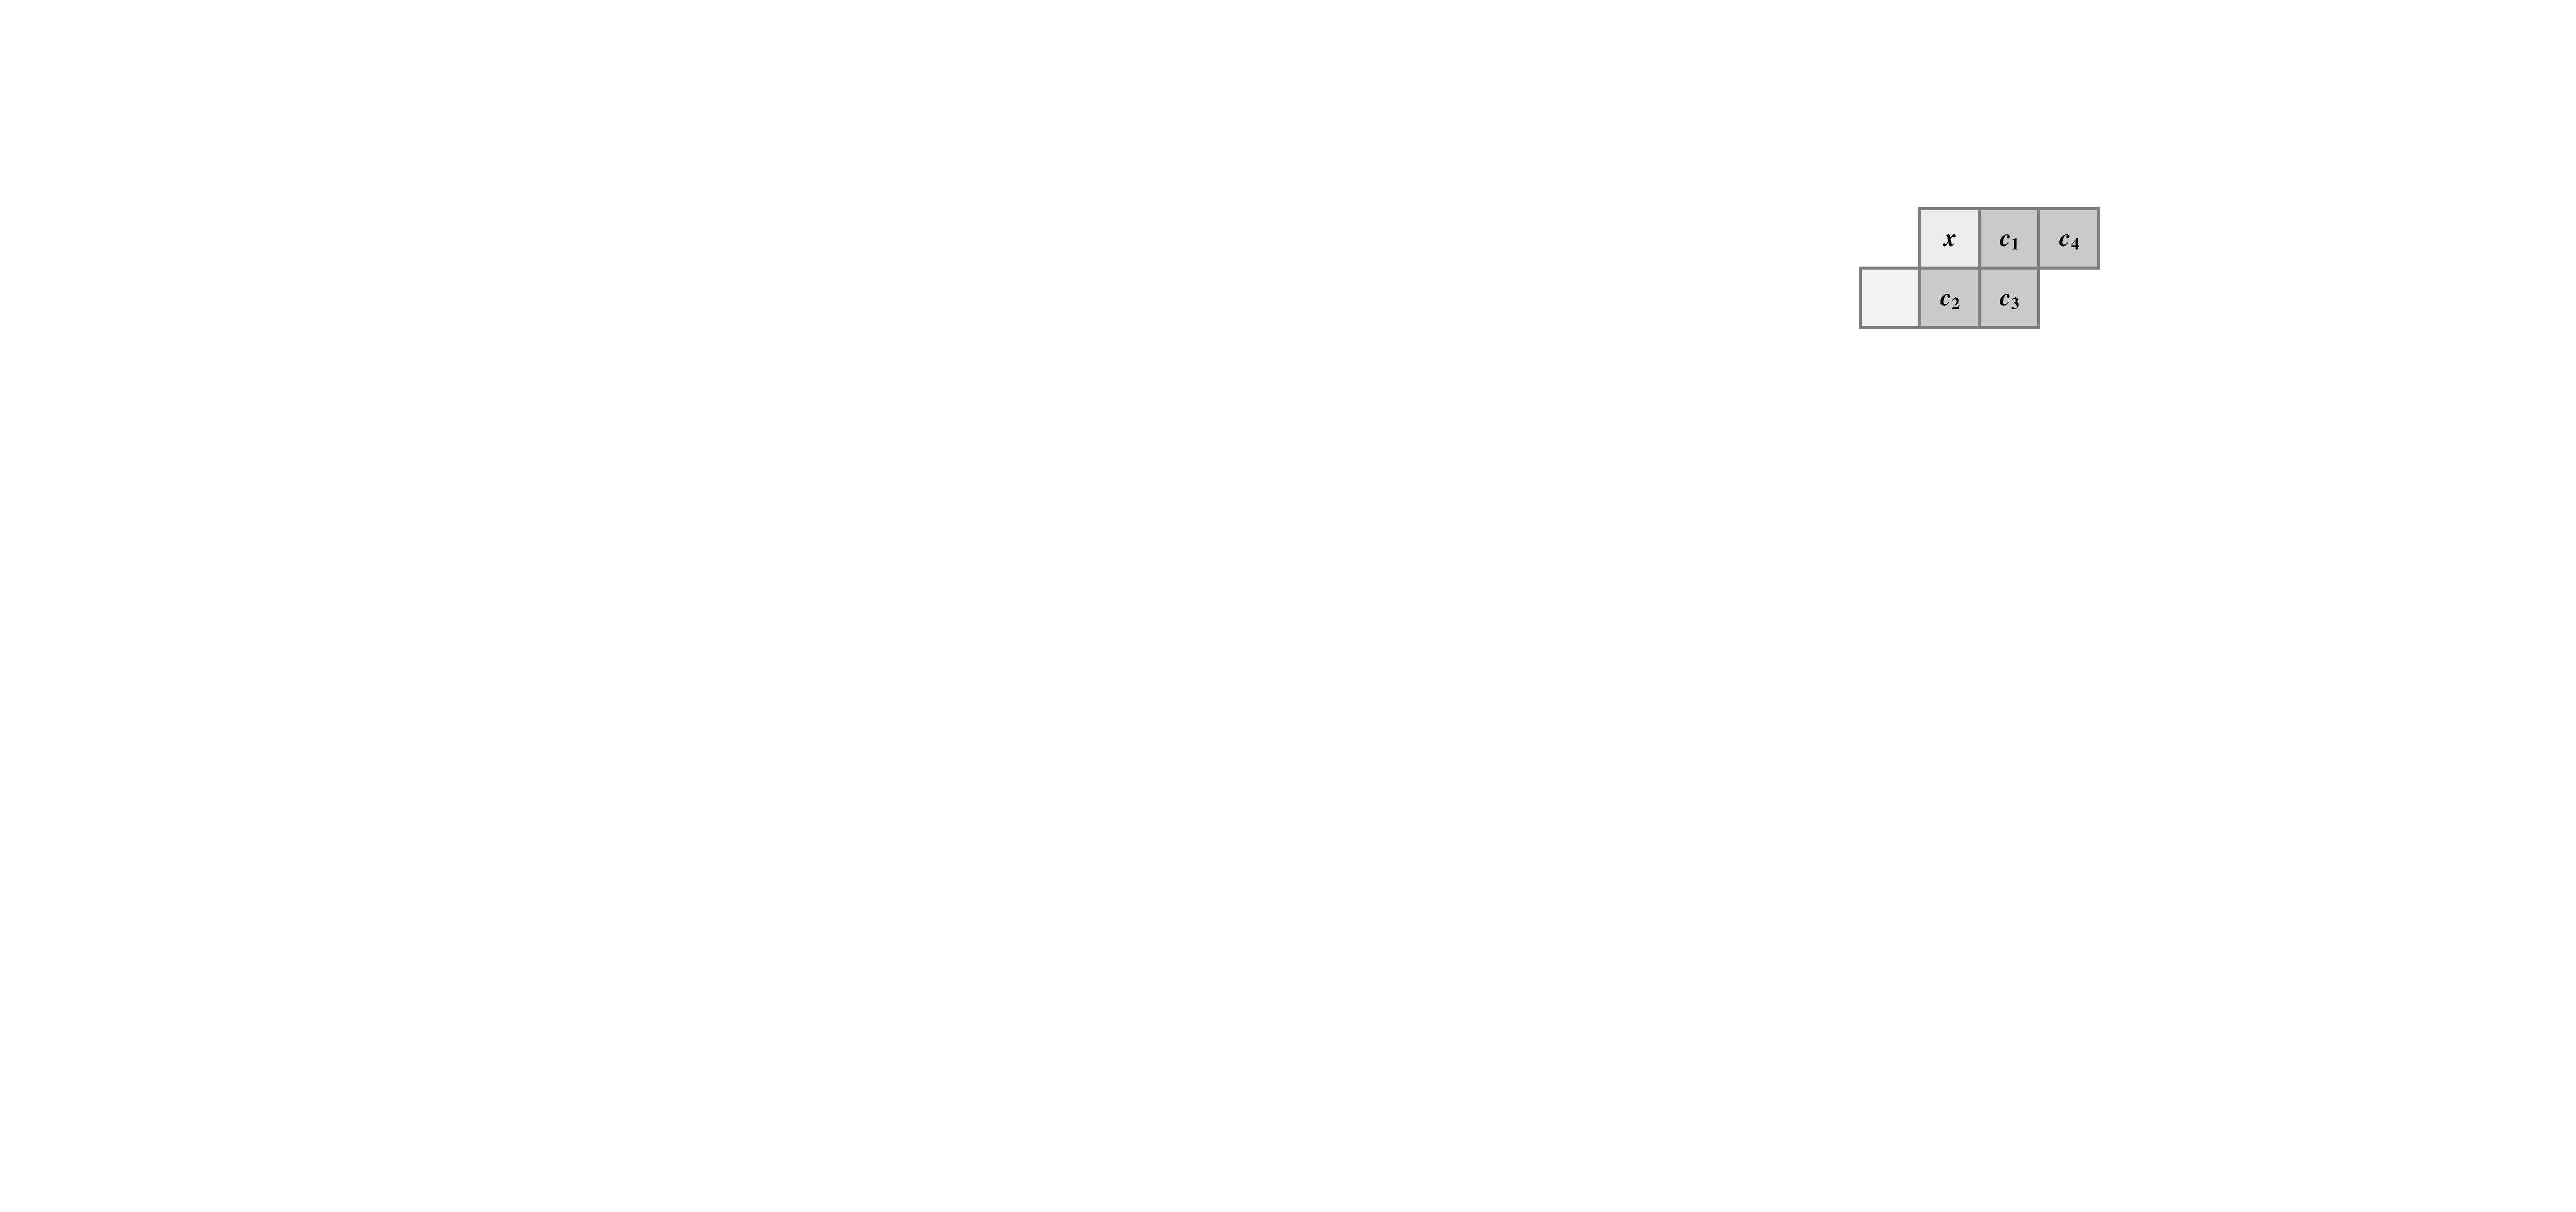
\includegraphics[width=1\textwidth]{figures/CN4a.pdf}
    \end{minipage}
}
\qquad\qquad
\subfigure[Proposed, $n=4$.]{
    \begin{minipage}[t]{0.2\linewidth}
    \centering
    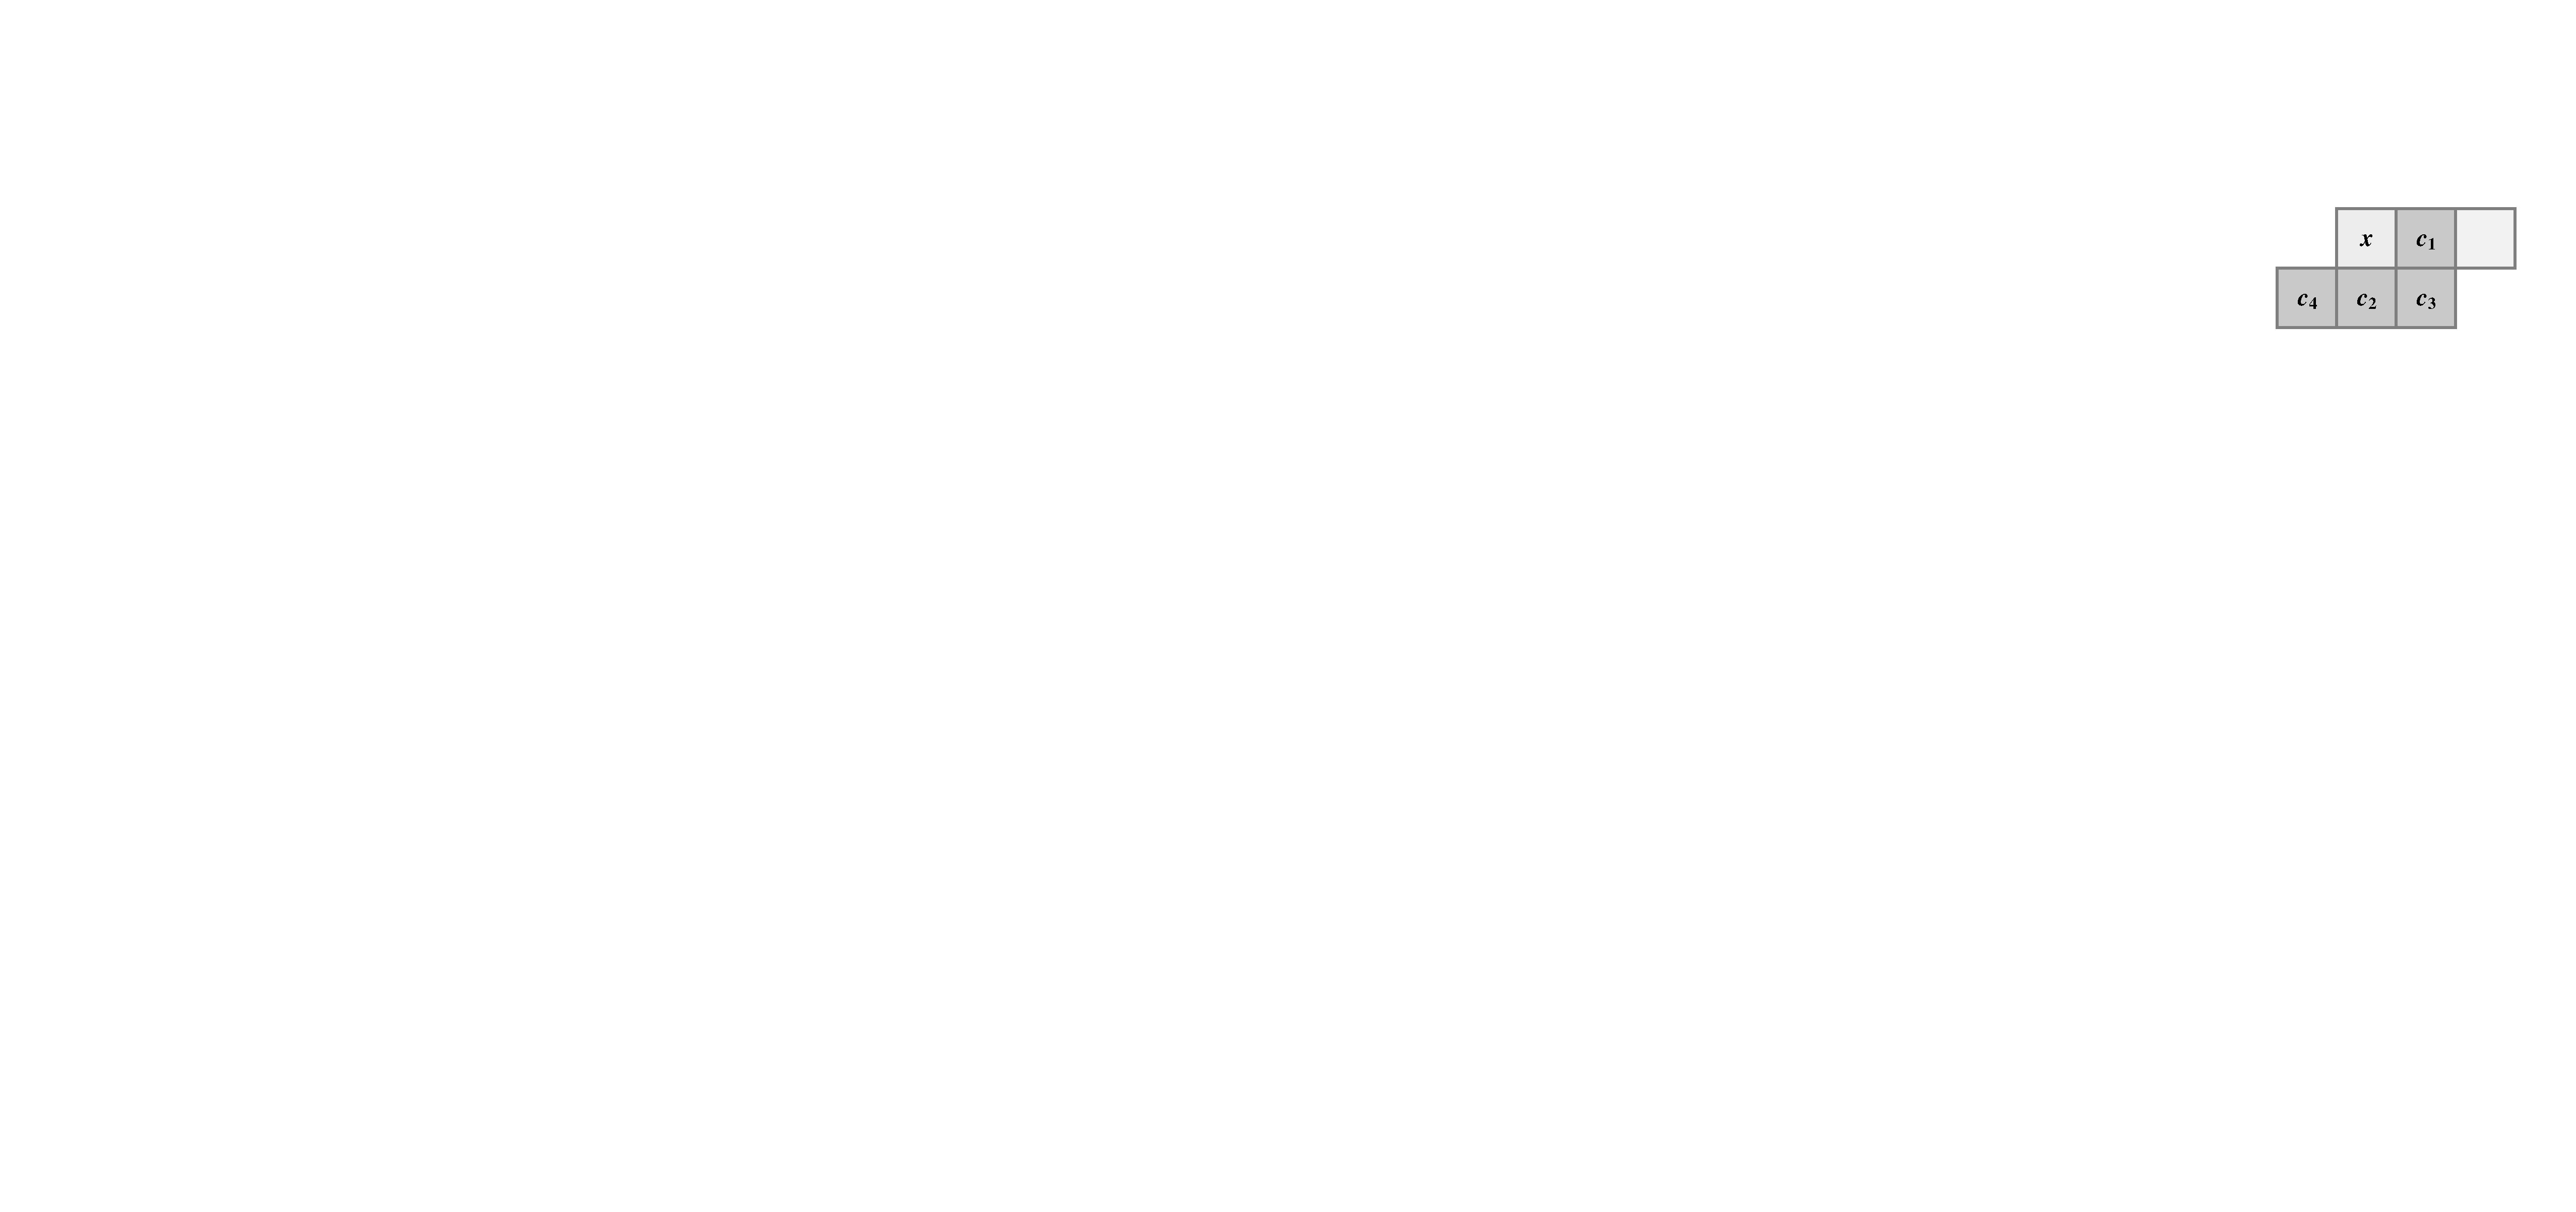
\includegraphics[width=1\textwidth]{figures/CN4b.pdf}
    \end{minipage}
}

\subfigure[PPVO, $n=8$]{
    \begin{minipage}[t]{0.2\linewidth}
    \centering
    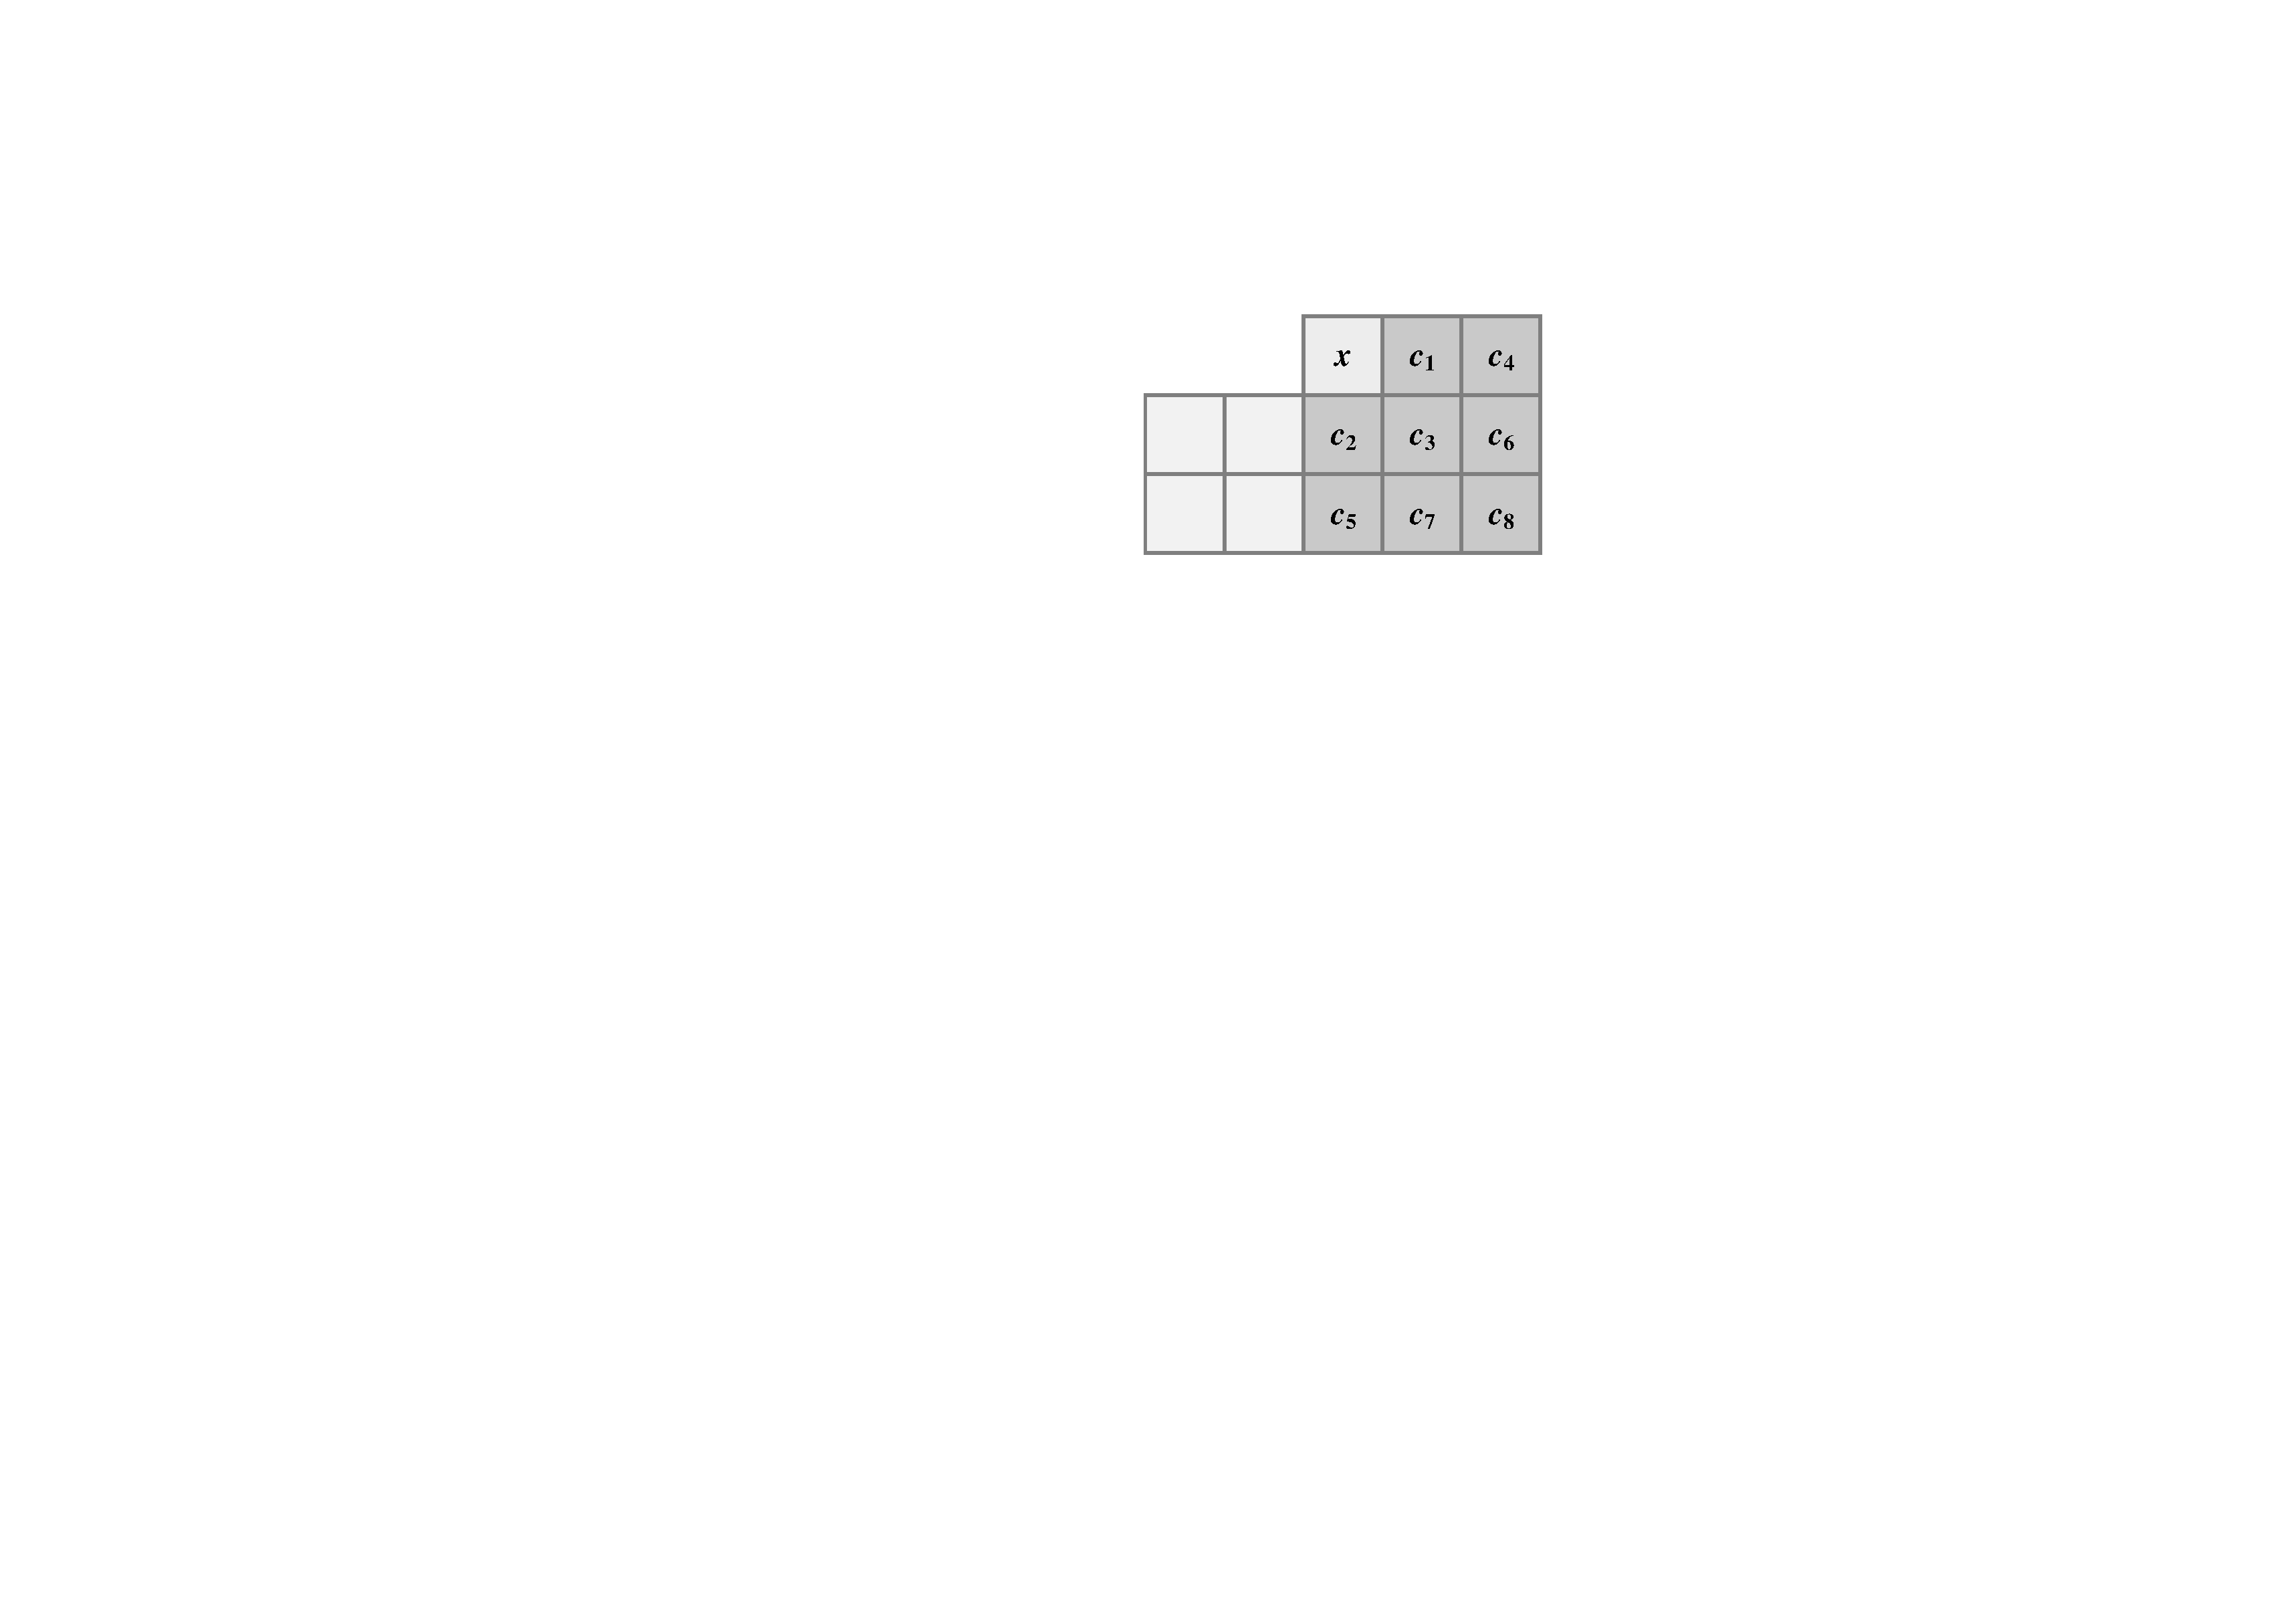
\includegraphics[width=1\textwidth]{figures/CN8a.pdf}
    \end{minipage}
}
\qquad\qquad
\subfigure[Proposed, $n=8$.]{
    \begin{minipage}[t]{0.2\linewidth}
    \centering
    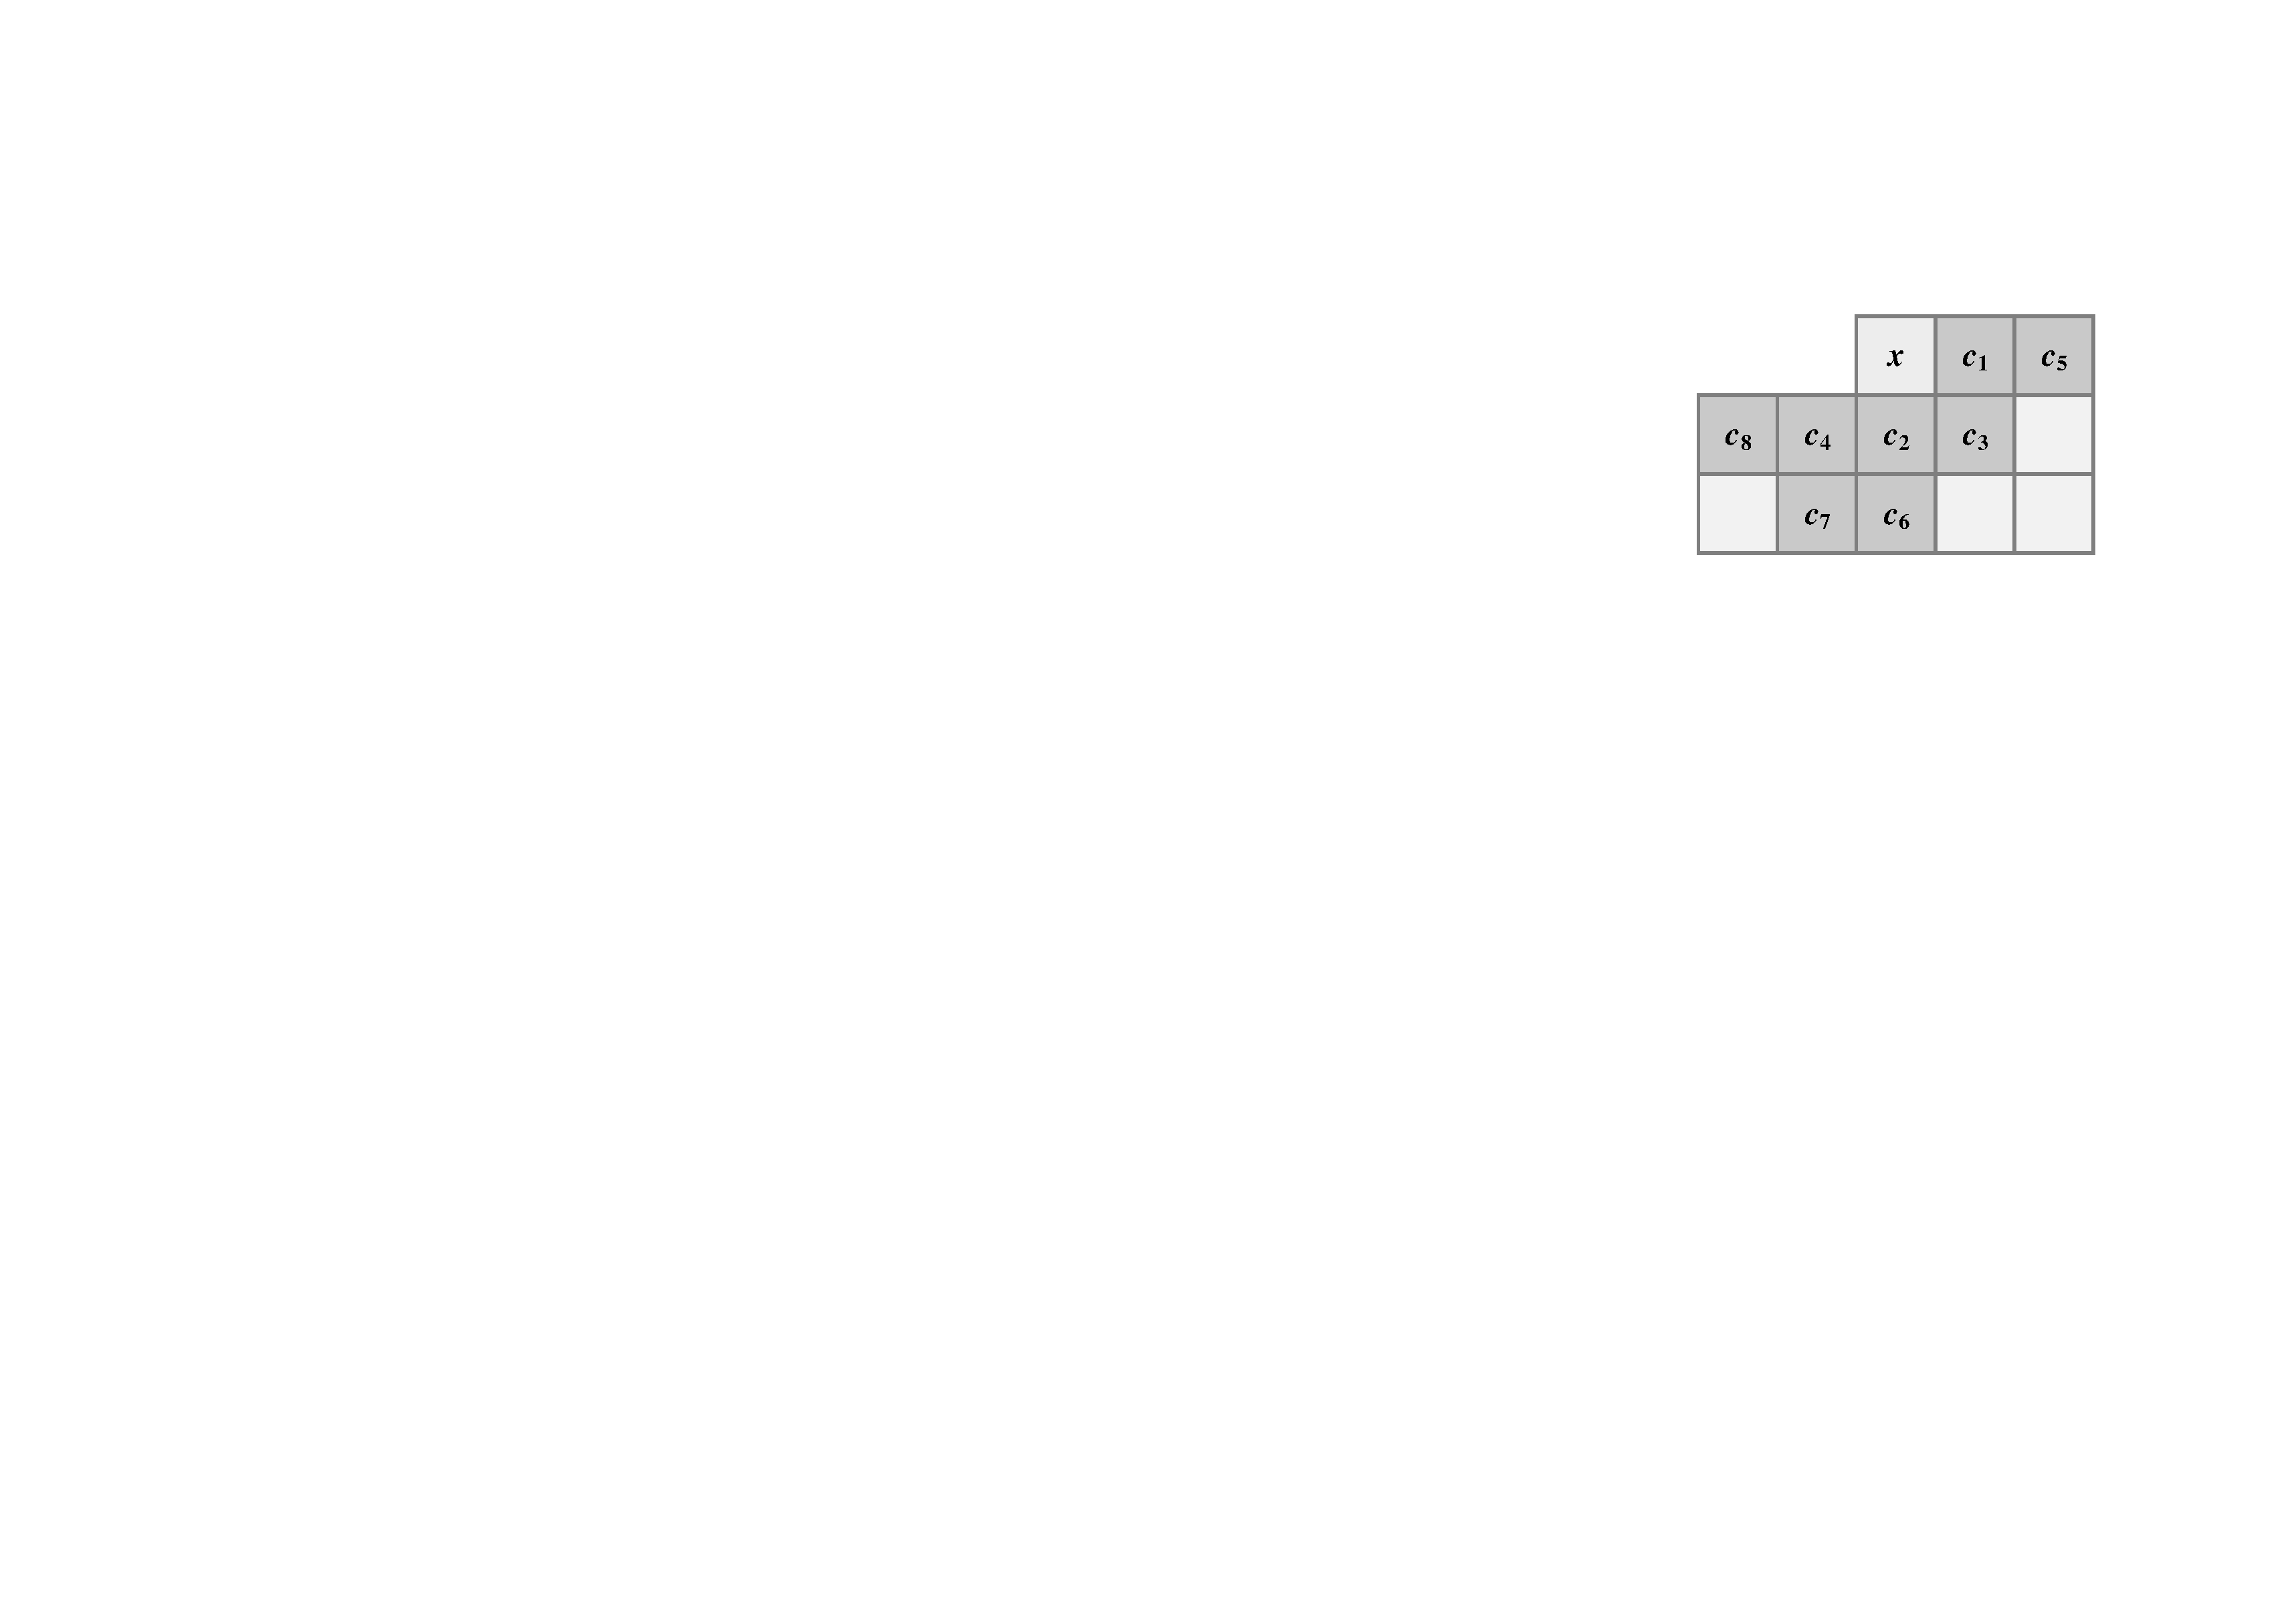
\includegraphics[width=1\textwidth]{figures/CN8b.pdf}
    \end{minipage}
}		
\centering
\caption{Prediction context of $x$, for PPVO and the proposed predictor with different number $n$ of context pixels.}
\label{Fig.Context}
\end{figure*}

\begin{figure}[t]
\centering
\subfigure[Lena, $n = 4$]{
    \begin{minipage}[t]{0.4\linewidth}
    \centering
    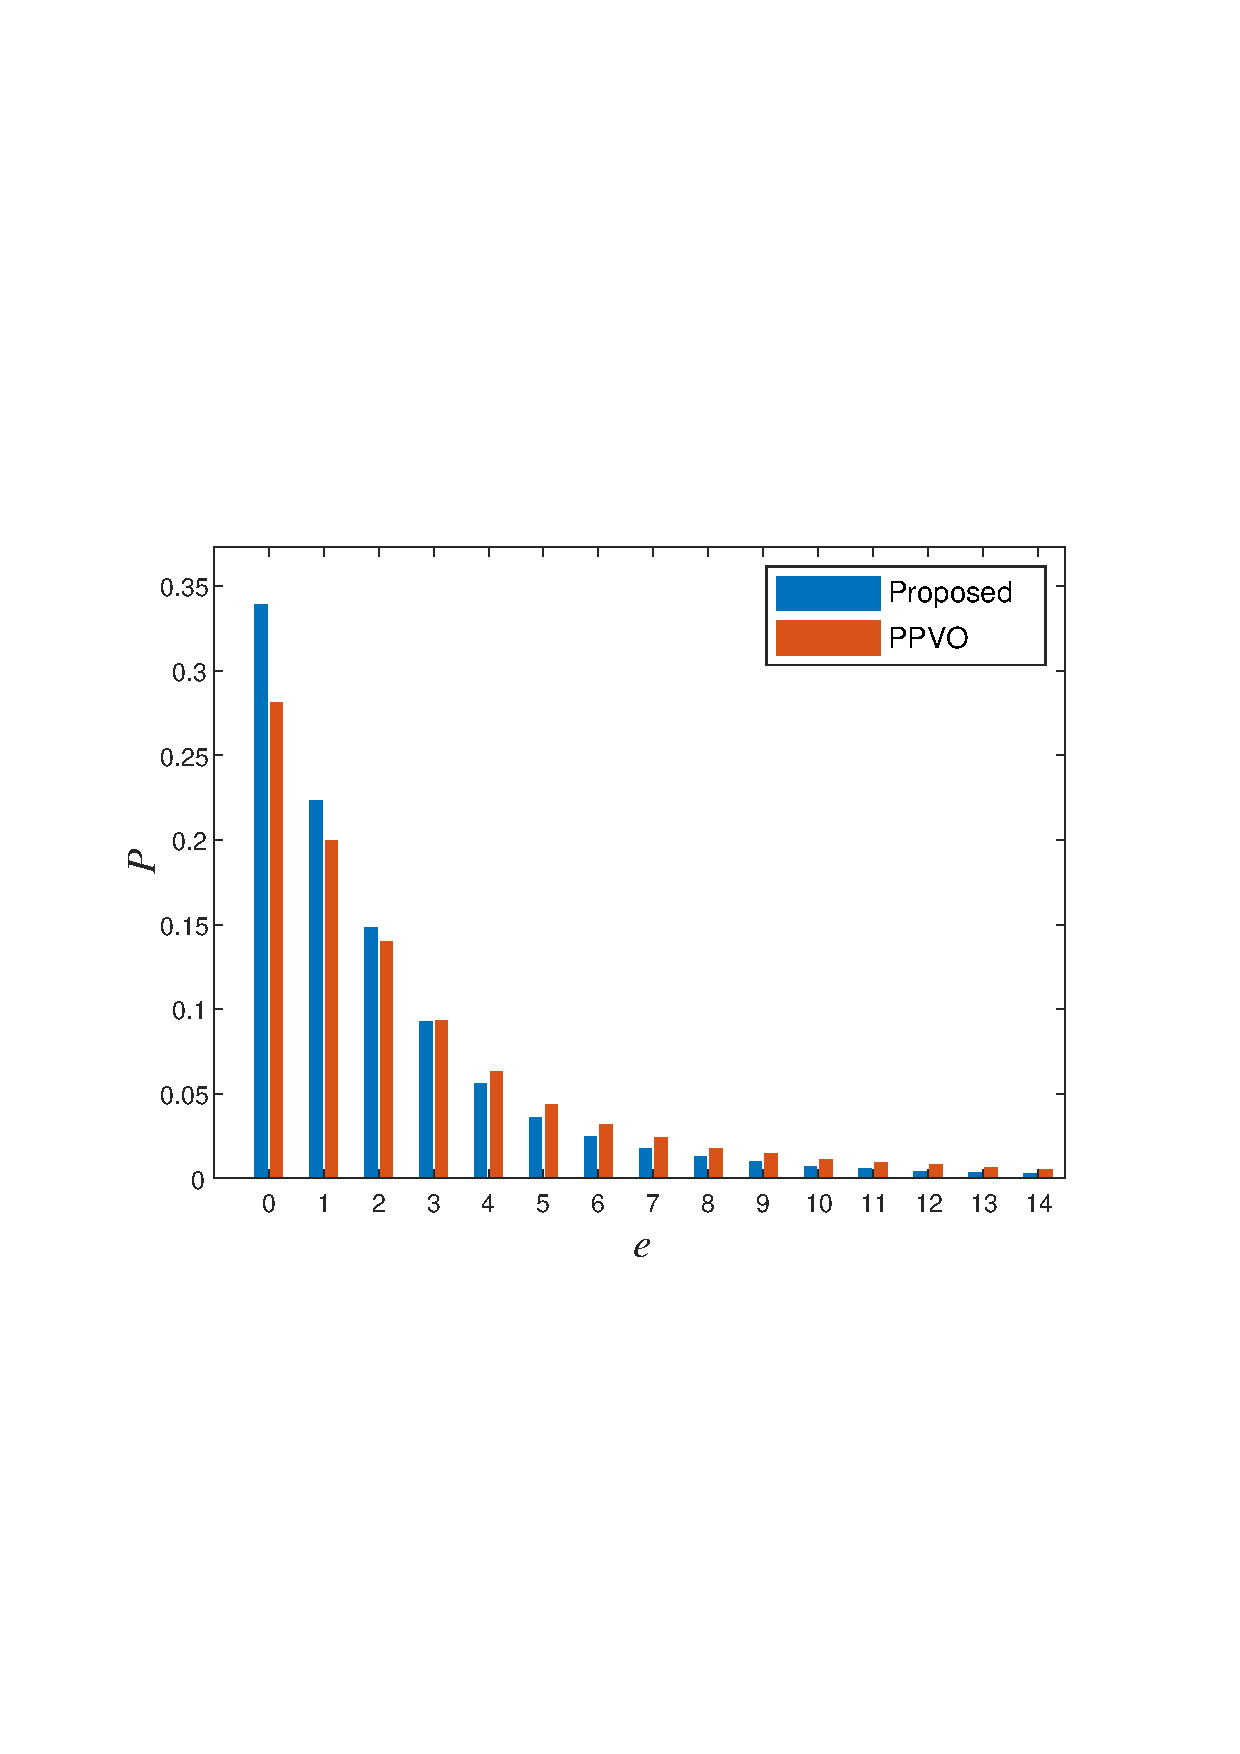
\includegraphics[width=1\textwidth]{figures/Comp4Lena.pdf}
    \end{minipage}
}
\qquad
\subfigure[Baboon, $n = 4$]{
    \begin{minipage}[t]{0.4\linewidth}
    \centering
    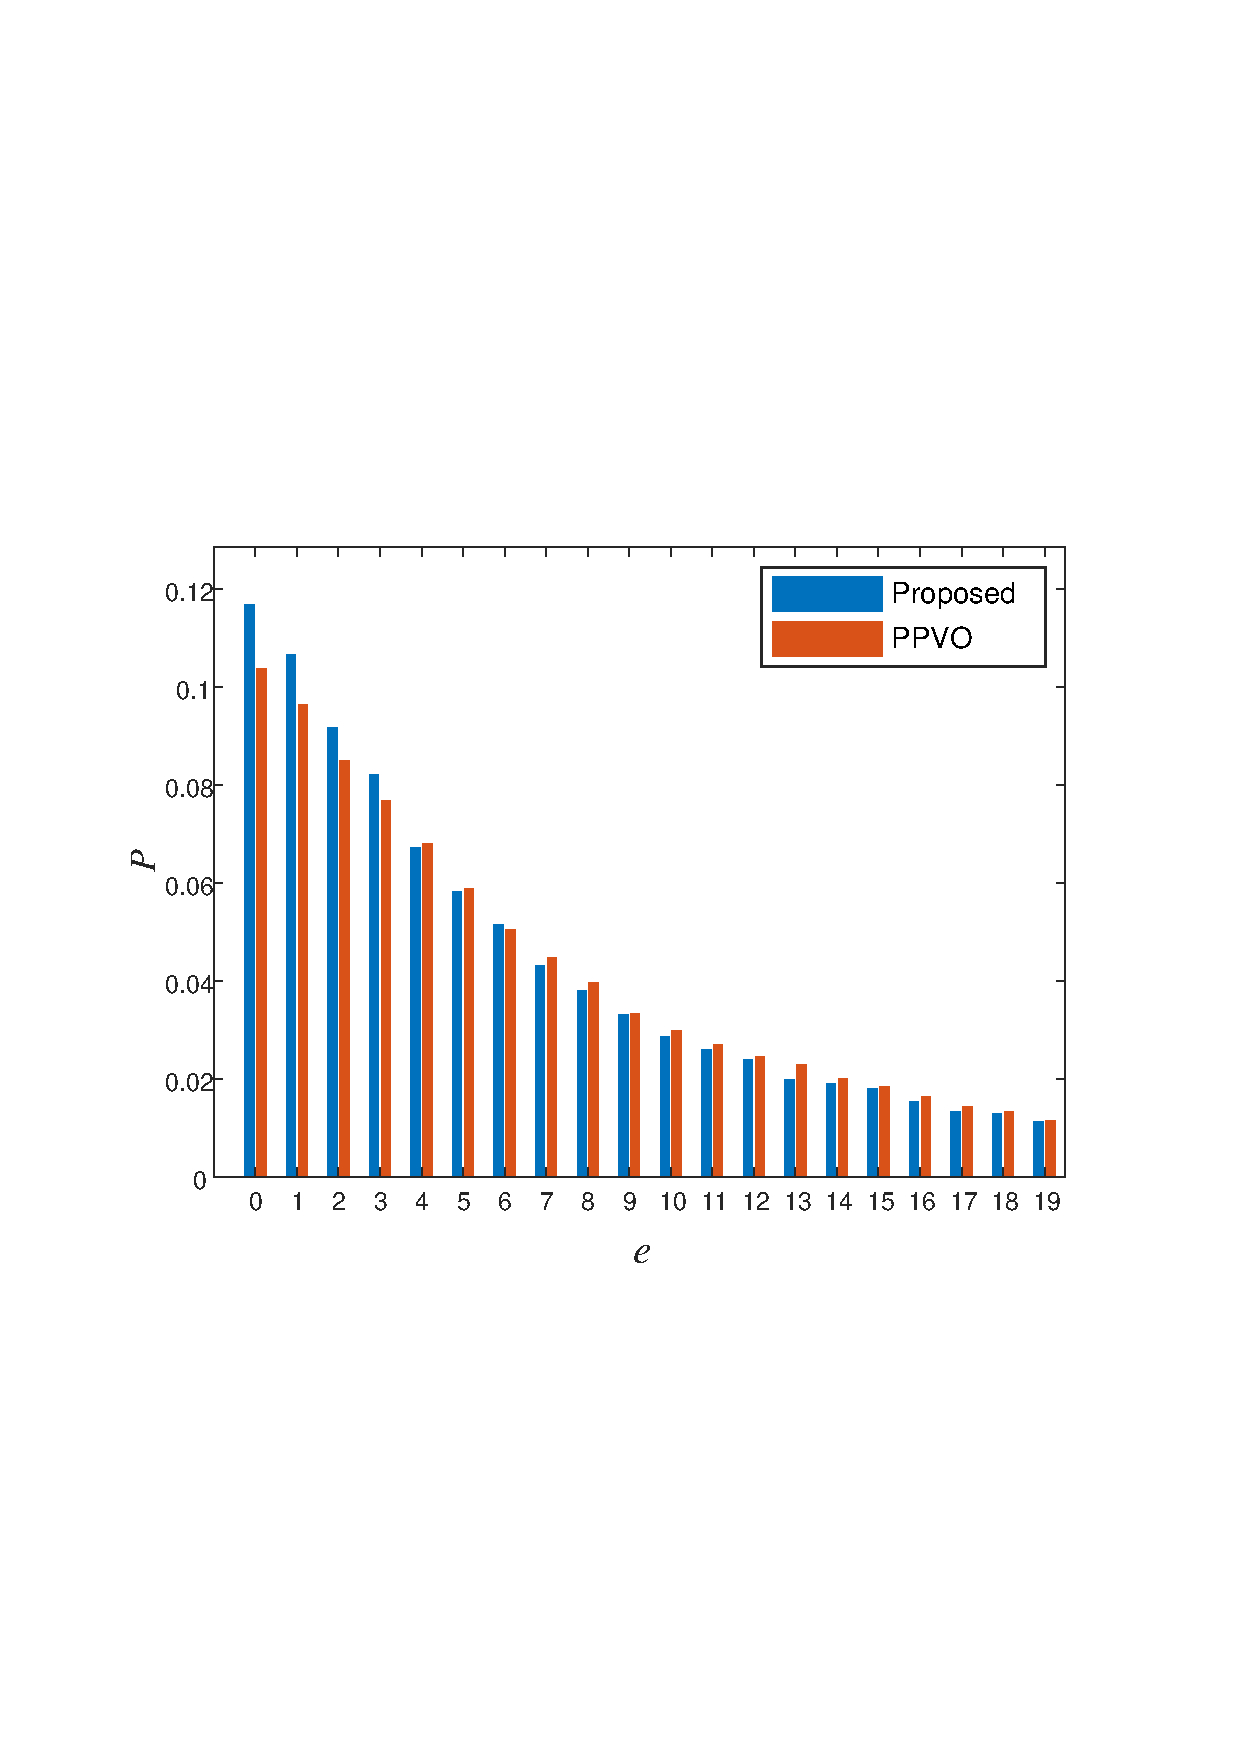
\includegraphics[width=1\textwidth]{figures/Comp4Baboon.pdf}
    \end{minipage}
}
\subfigure[Lena, $n = 8$]{
    \begin{minipage}[t]{0.4\linewidth}
    \centering
    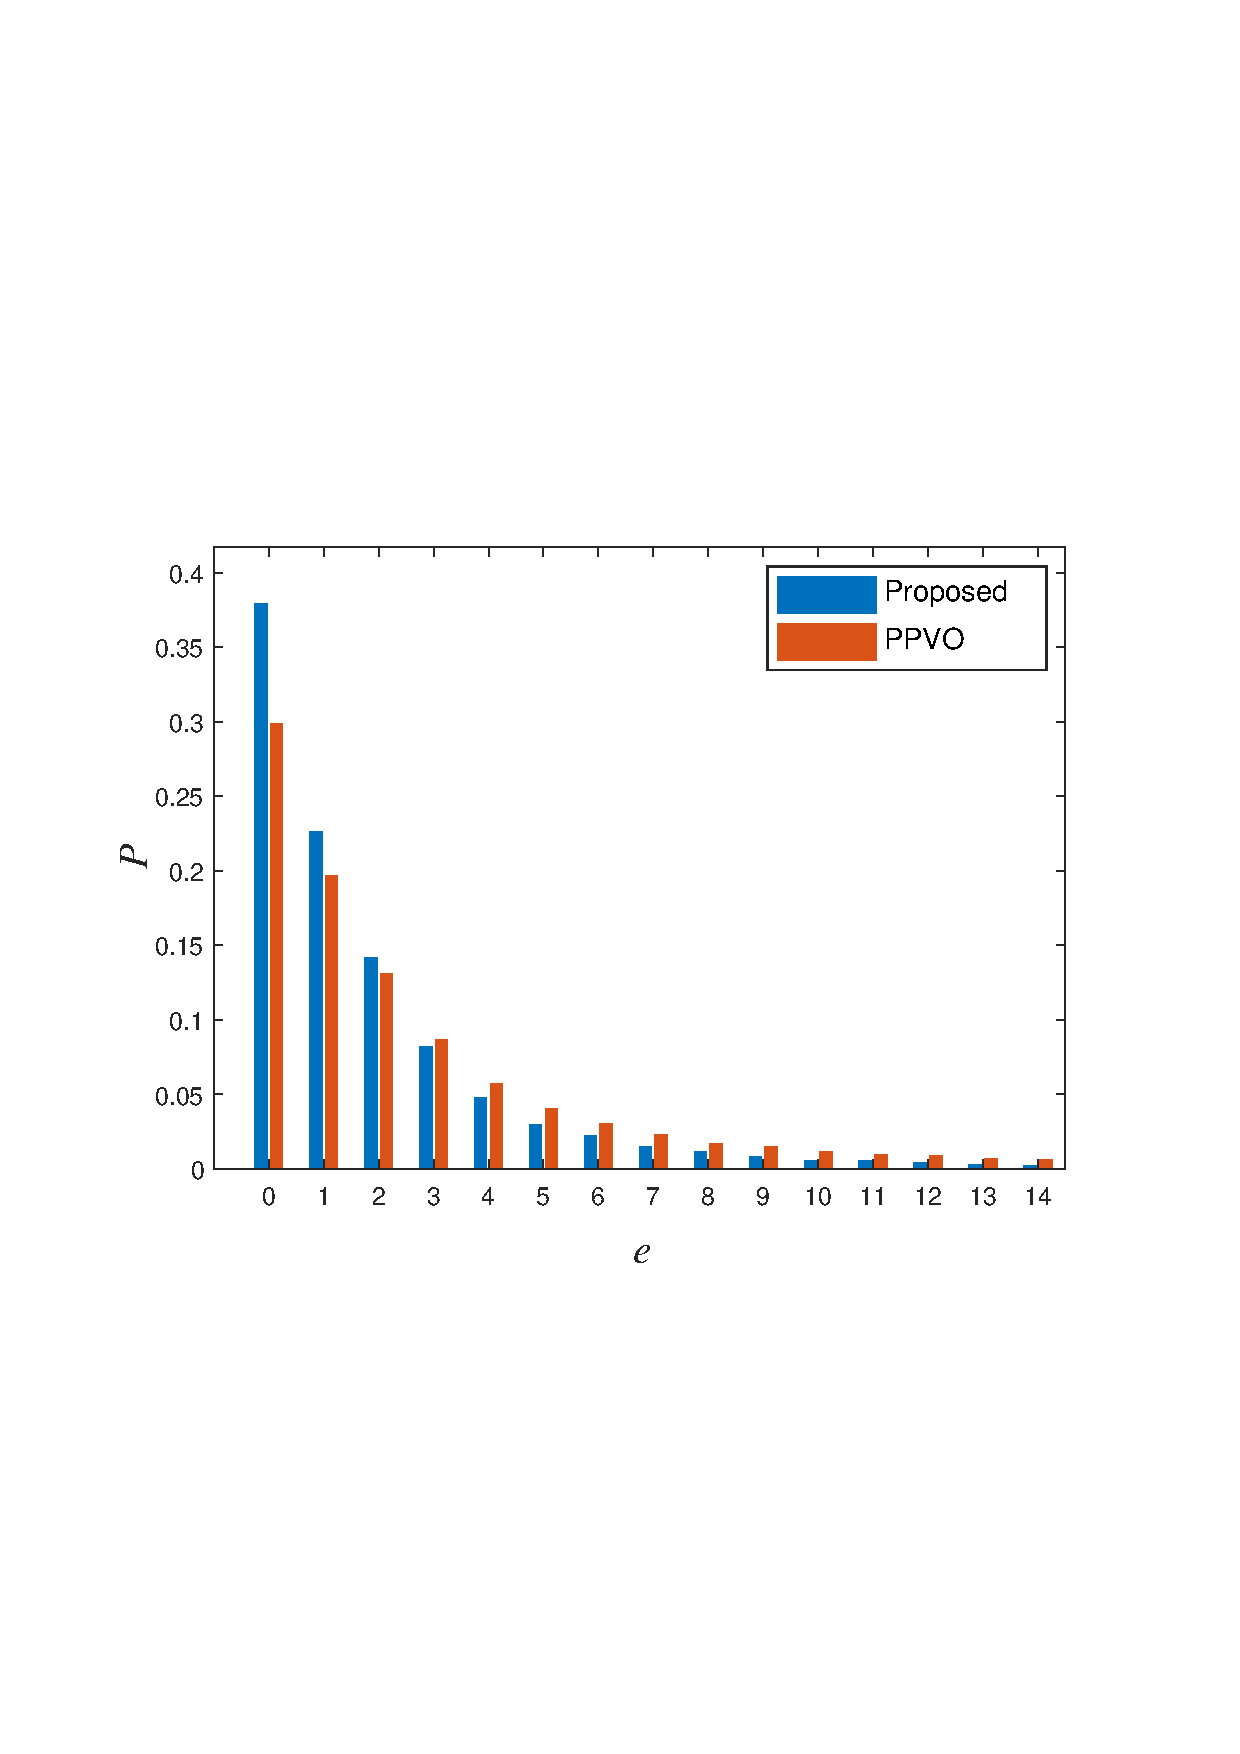
\includegraphics[width=1\textwidth]{figures/Comp8Lena.pdf}
    \end{minipage}
}
\qquad
\subfigure[Baboon, $n = 8$]{
    \begin{minipage}[t]{0.4\linewidth}
    \centering
    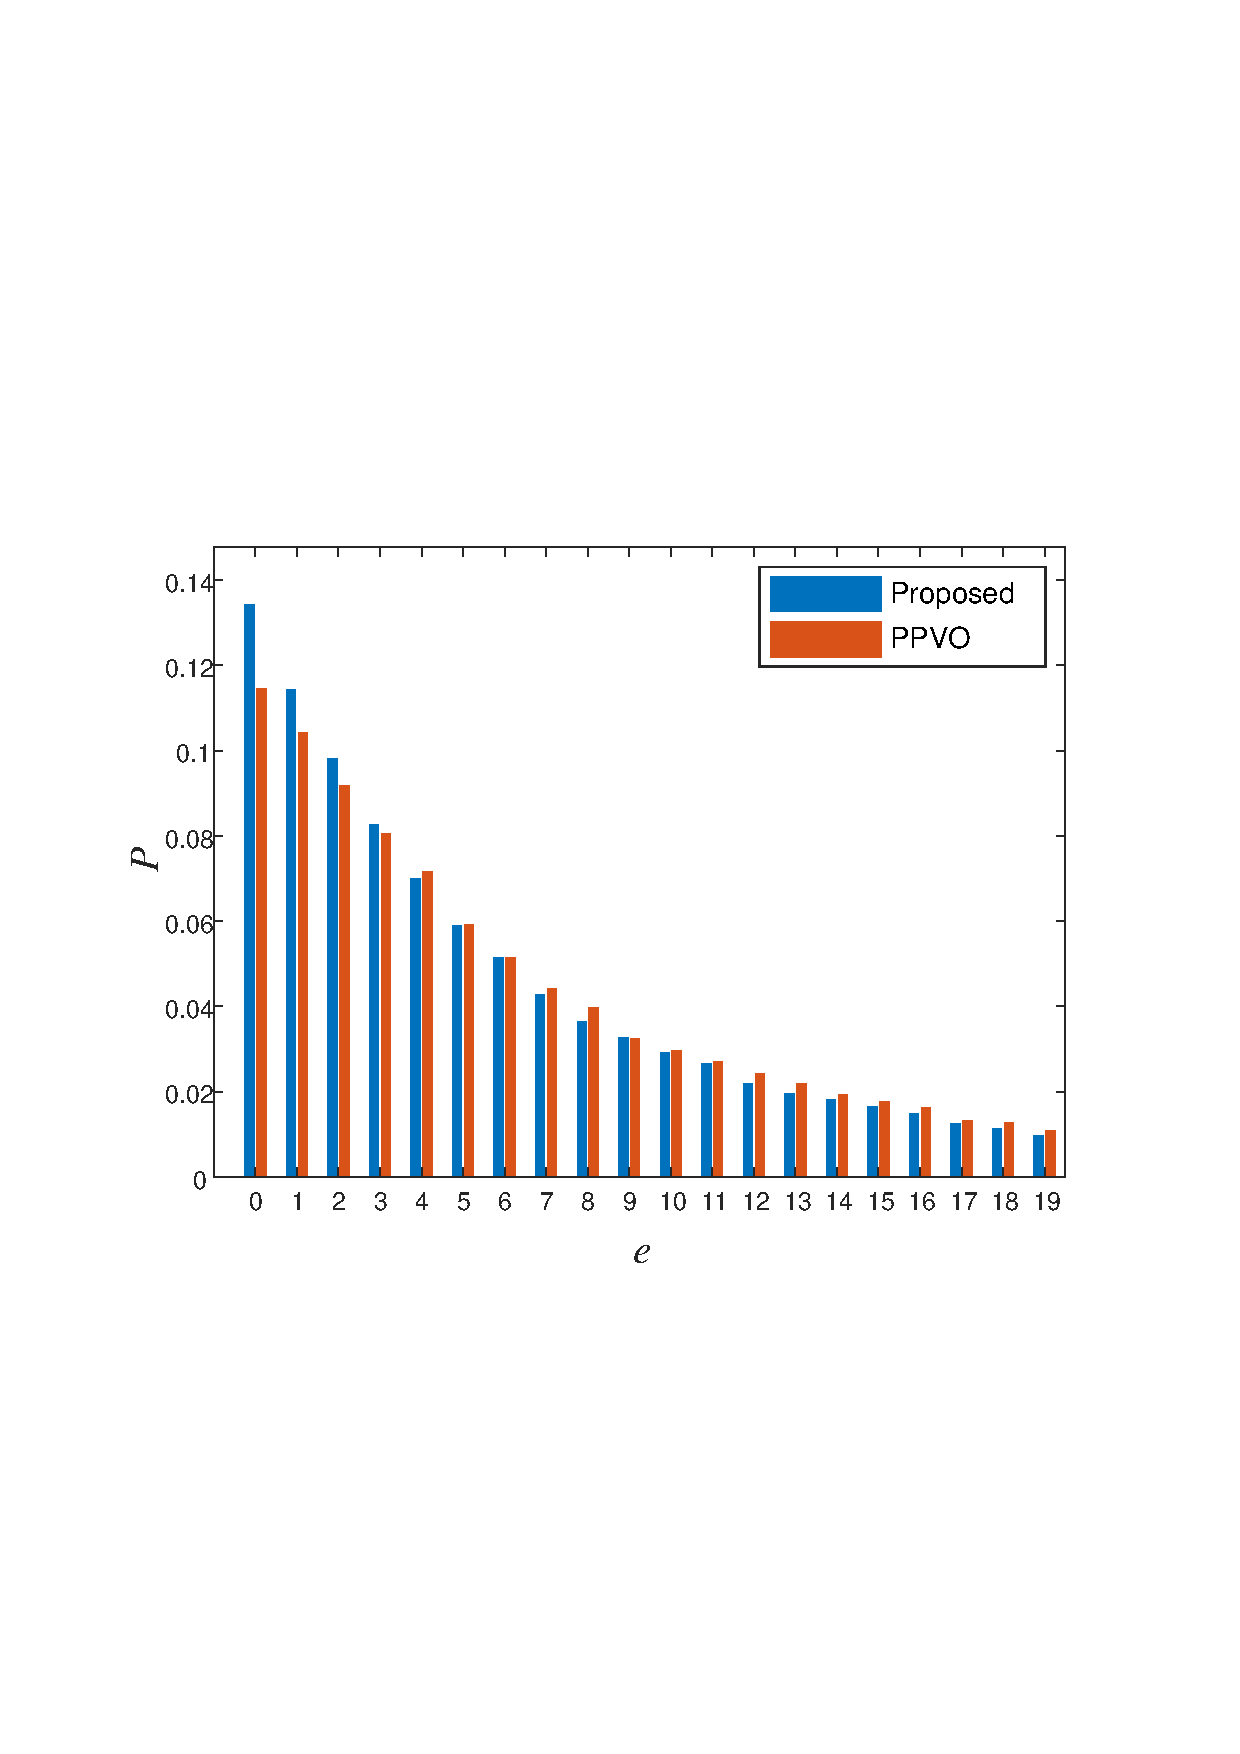
\includegraphics[width=1\textwidth]{figures/Comp8Baboon.pdf}
    \end{minipage}
}
\caption{Comparison of normalized PEHs derived from PPVO \cite{Qu2015PPVO} and the proposed predictor, for images Lena and Baboon with different prediction contexts shown in Fig. \ref{Fig.Context}.}
\label{Fig.ComparisonEPPVO}
\end{figure}

An experiment is conducted to verify the effectiveness of the proposed predictor. The standard $512 \times 512$ sized gray-scale images Lena and Baboon are used here. Fig. \ref{Fig.ComparisonEPPVO} shows the comparison between the normalized PEHs derived from PPVO and the proposed predictor. Two different prediction contexts with $n = 4$ and $n = 8$ are compared. Specifically, for PPVO, the prediction contexts are the ones shown in Fig. \ref{Fig.Context}(a) and (c). For the proposed predictor, we use the contexts shown in Fig. \ref{Fig.Context}(b) and (d) for prediction. Notice that, only the PEHs based on the pixels in $S_1 \cup S_4$ are shown in Fig. \ref{Fig.ComparisonEPPVO} for simplicity.
According to these figures, compared with the PEH derived from PPVO, the one based on the proposed predictor with blue color has higher peak at bin 0 in each case, and the proposed PEHs are sharper.
Moreover, the proportion of shifted pixels defined in \cite{Li2013PVO} is used to measure the statistical characteristics of PEH in a quantitative way, and it is calculated by
\begin{equation}\label{eq:Pshift}
    P=\frac{\#\{{\rm shifted\ pixels}\}}{\#\{{\rm expanded\ or\ shifted\ pixels}\}} = \frac{\sum_{i > 0}h(i)}{h(0) + \sum_{i > 0}h(i)}
\end{equation}
where $h$ represents the generated PEH. Obviously, the smaller the value of $P$, the sharper the PEH and hence the better the embedding performance. In Fig. \ref{Fig.ComparisonEPPVO}(a) and (c), for image Lena, when $n=4$, the values of $P$ corresponding to PPVO and the proposed predictor are 0.72 and 0.66, respectively. When $n=8$, $P$ equals 0.7 and 0.62 with these two predictors. It is obvious that, the values of $P$ are decreased based on the proposed predictor, indicating that the embedding distortion can be decreased as well. Besides, similar results also can be observed on the PEHs of image Baboon. In summary, the proposed predictor provides more accurate prediction results, and hence the embedding performance can be improved.



\subsection{Multi-size based Embedding Method for MHM}\label{sec:3.2}
As mentioned above, in PPVO \cite{Qu2015PPVO}, the number of context pixels used for the prediction of each pixel is fixed, and the value of $n$ is experimentally chosen from 1 to 15. However, different number of context pixels can lead to different embedding performance. In order to analyze the impact of different $n$ on the embedding performance, we set $n\leq 24$ and choose four different context vectors for experiments. Specifically, the context vectors are $C_1 = \{c_1, ..., c_4\}$, $C_2 = \{c_1, ..., c_{10}\}$, $C_3 = \{c_1, ..., c_{18}\}$ and $C_4 = \{c_1, ..., c_{24}\}$, as shown in Fig. \ref{Fig.Context3}. Specific analysis is conducted based on the threshold-capacity curves and the curves about the threshold with the proportion of shifted pixels. Fig. \ref{Fig.Eval} shows the comparison results between the context vectors $C_1$ and $C_2$. Here, the threshold means the local complexity threshold used for pixel selection, and only pixels whose local complexity is smaller than the threshold are used for embedding. Note that, for a target pixel, the local complexity, denoted as NL, is calculated by the sum of the absolute values of the differences between each pair of adjacent context pixels in the horizontal and vertical directions. In this experiment, the context pixel region used for NL calculation is shown in Fig. \ref{Fig.Context3}(b). Besides, the proportion of shifted pixels is exactly the value of $P$ defined in \eqref{eq:Pshift}. And, the embedding capacity is equal to the number of prediction-errors valued 0. According to the comparison results shown in Fig. \ref{Fig.Eval}, several observations are given as follows.

%Based on the consideration of the complexity of traditional RDH embedding, the comparison of threshold-capacity curves and threshold-proportion curves are shown in Fig. \ref{Fig.Eval}(a) and Fig. \ref{Fig.Eval}(b) as well.Here the proportion indicates the proportion of shifted pixels refined by (\ref{eq:Pshift}). And the threshold $T$ is set to choose the smooth pixels whose complexity ${\rm NL} < T$ to generate PEH so that all secret data can just be embedded. The complexity of the current pixel is evaluated by the sum of the absolution differences of the horizontal and vertical of every two adjacent pixels belong to the corresponding context. Besides, the capacity is defined as the occurrence of bin 0 of the generated PEH.

\begin{figure*}
\subfigure[$C_1$ of $n = 4$]{
    \begin{minipage}[t]{0.218\linewidth}
    \centering
    
\includegraphics[width=1\textwidth]{figures/C1.pdf}
    \end{minipage}
}
\subfigure[$C_2$ of $n = 10$]{
    \begin{minipage}[t]{0.218\linewidth}
    \centering
    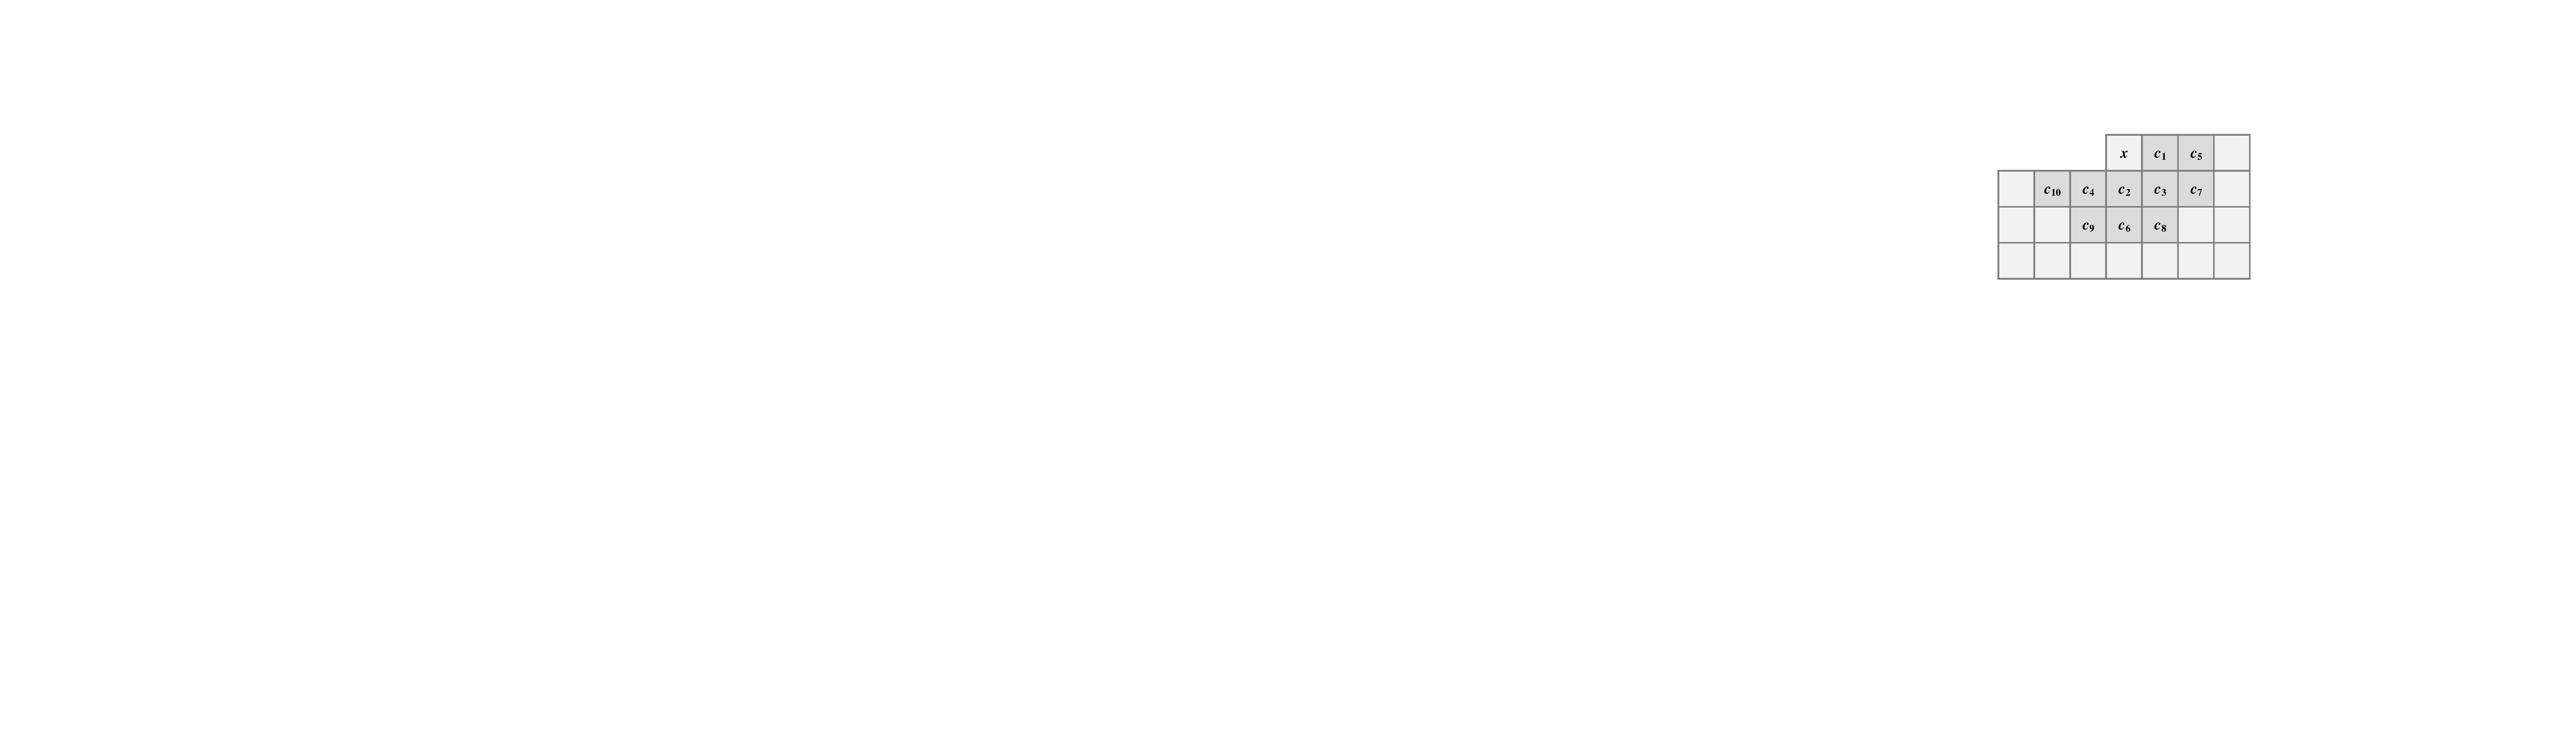
\includegraphics[width=1\textwidth]{figures/C2.pdf}
    \end{minipage}
}
\subfigure[$C_3$ of $n = 18$]{
    \begin{minipage}[t]{0.218\linewidth}
    \centering
    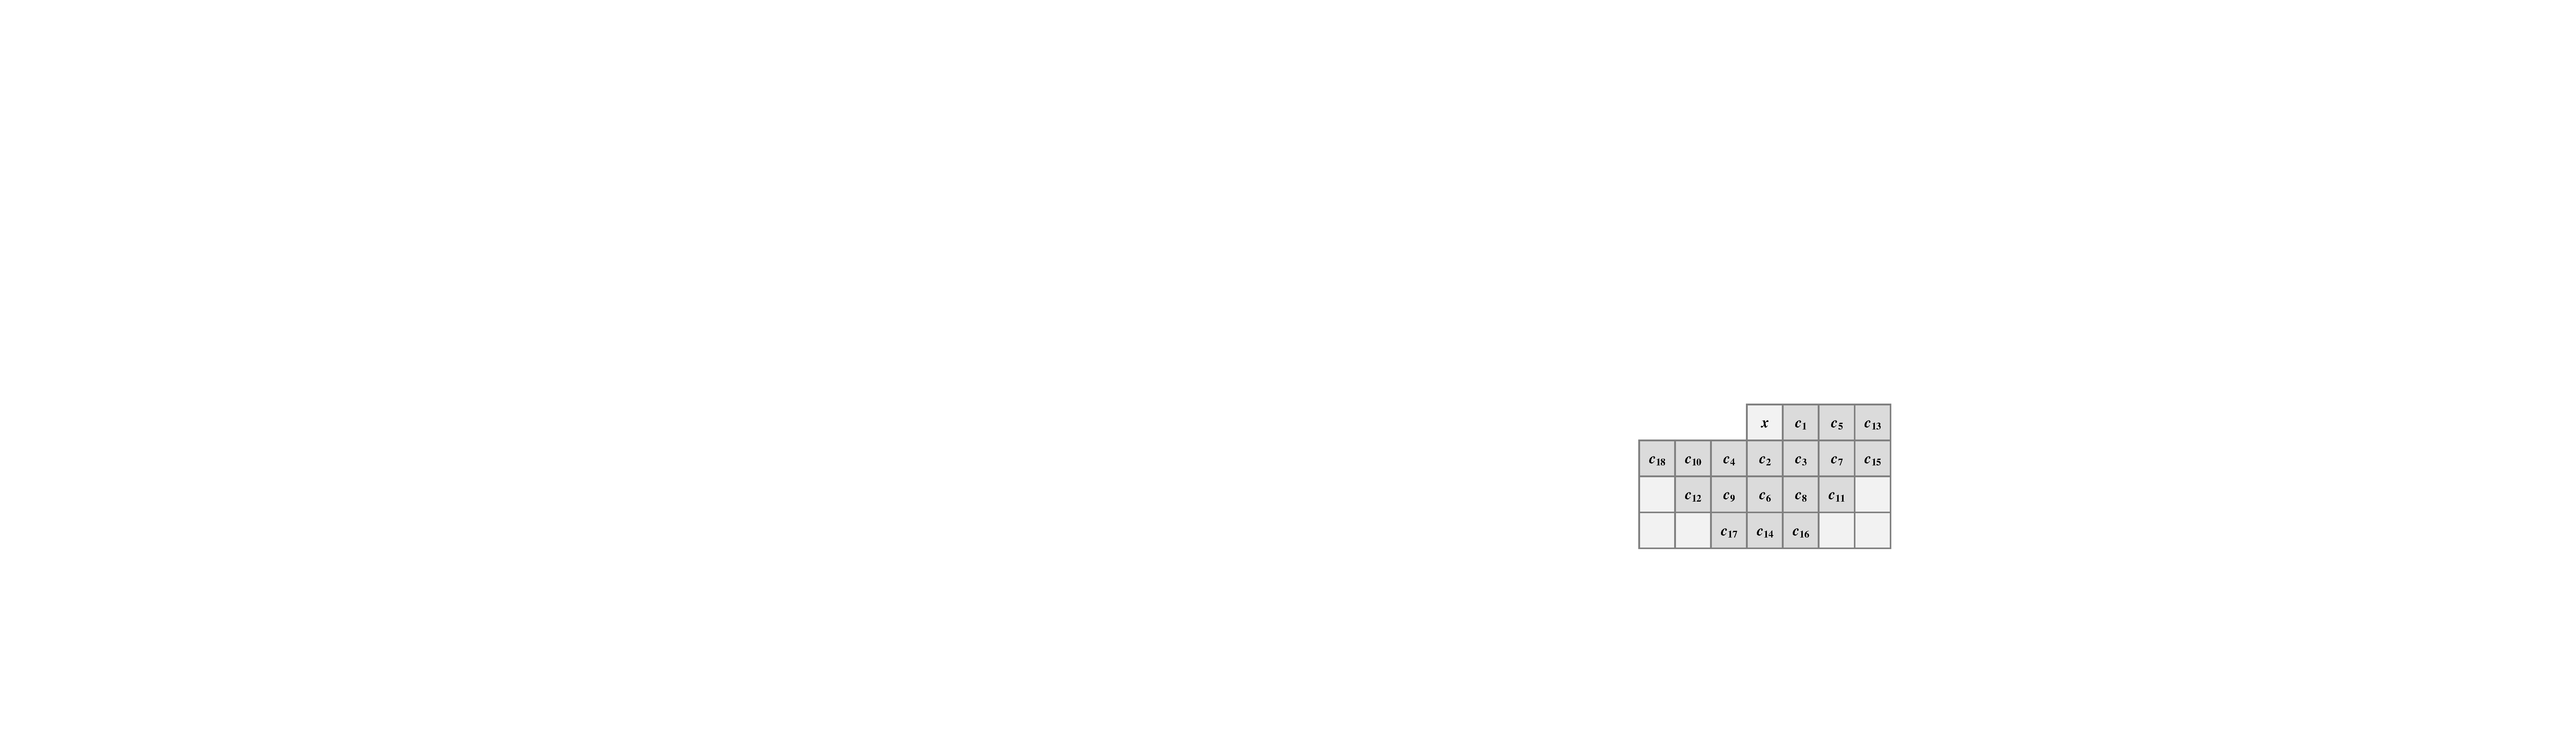
\includegraphics[width=1\textwidth]{figures/C4.pdf}
    \end{minipage}
}
\subfigure[$C_4$ of $n = 24$]{
    \begin{minipage}[t]{0.218\linewidth}
    \centering
    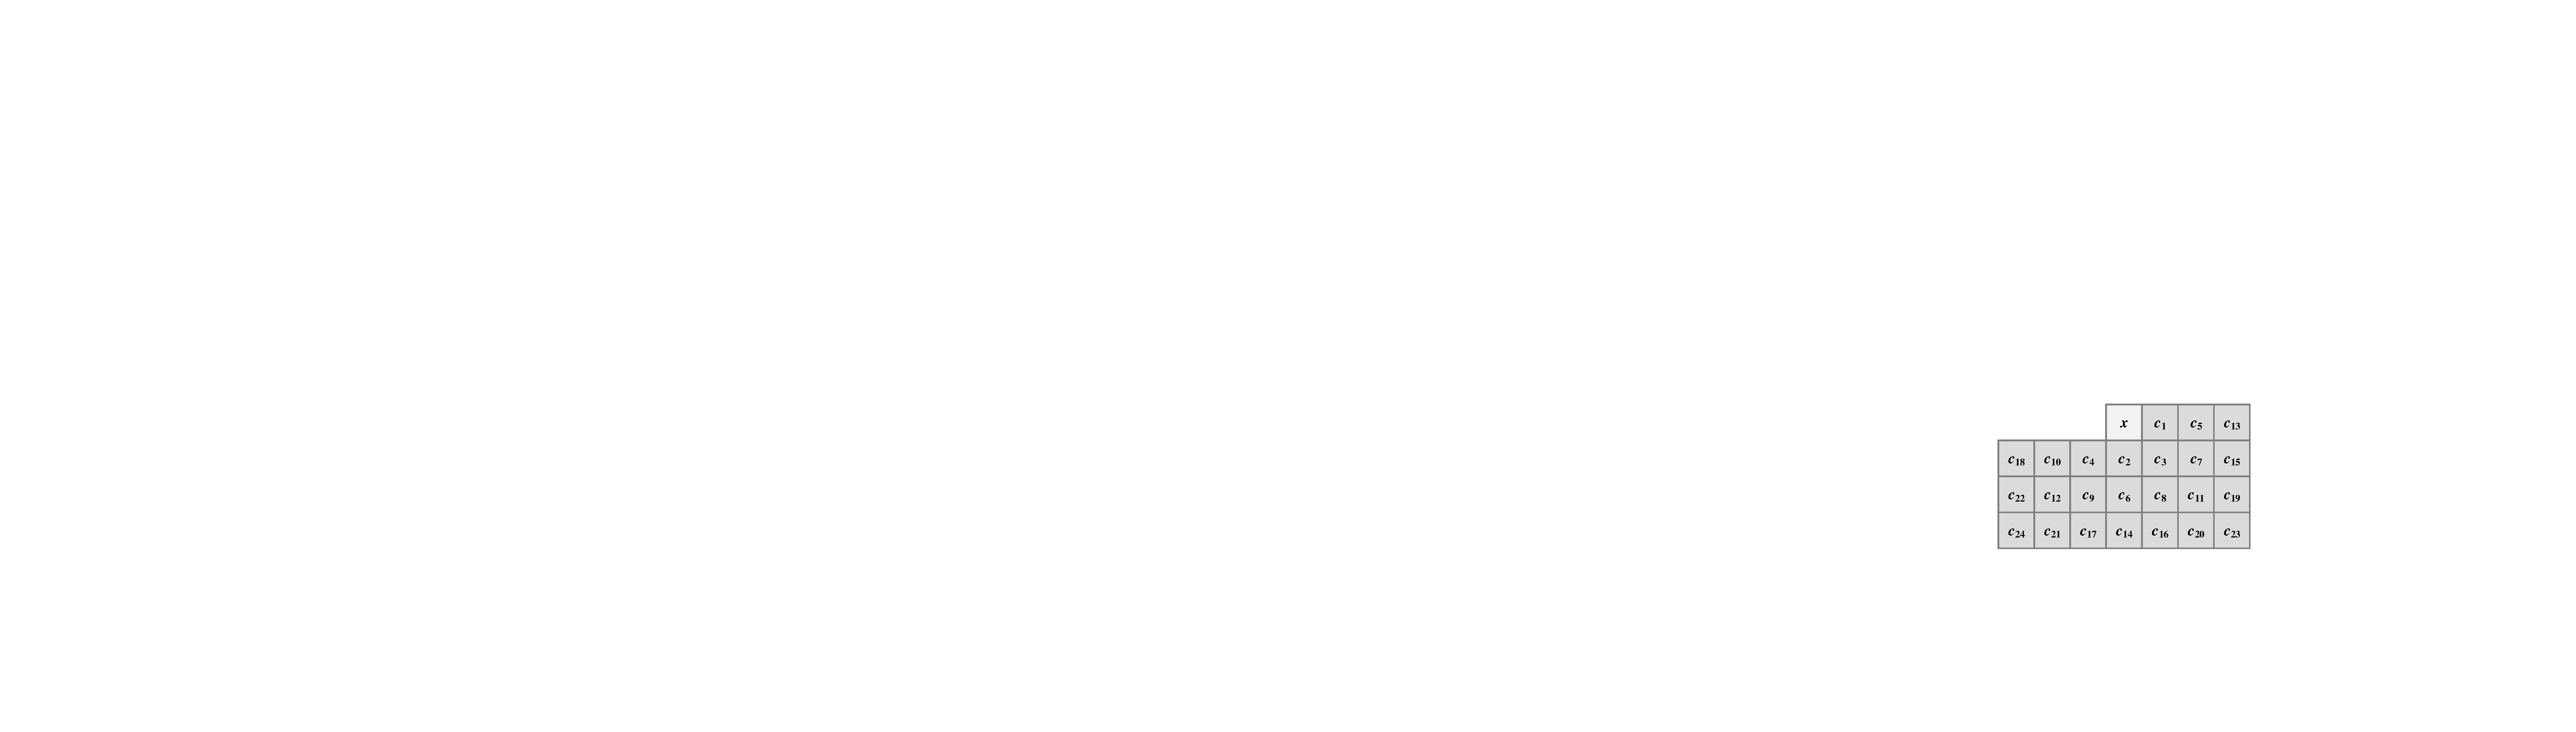
\includegraphics[width=1\textwidth]{figures/C3.pdf}
    \end{minipage}
}
\centering
\caption{Context pixels of $x$ by Extended PPVO.}
\label{Fig.Context3}
\end{figure*}

\begin{enumerate}
  \item In Fig. \ref{Fig.Eval}(a), for a fixed threshold, the maximum embedding capacity derived based on $C_1$ is much larger than that based on $C_2$. The main reason is that, when $n$ is small, almost all the cover pixels are used for embedding while part of the pixels are skipped with large value of $n$ based on $C_2$.
  \item In Fig. \ref{Fig.Eval}(a), the embedding capacity is dramatically increased with the increase of the threshold at the beginning, especially for the curve corresponding to $C_1$, indicating that pixels belong to smooth areas are accurately predicted and they are more suitable for data embedding.
  \item According to Fig. \ref{Fig.Eval}(a) and (b), for a fixed threshold, although the embedding capacity corresponding to $C_2$ is smaller than $C_1$, the proportion of shifted pixels corresponding to $C_2$ is much smaller than that of $C_1$. In other words, the skipped pixels in the case of $C_2$ are difficult to be accurately predicted. Thus, they make little contribution on the improvement of the embedding performance.
\end{enumerate}
In a word, large embedding capacity is obtained by using small number of context pixels, but corresponding distortion is also increased due to the inaccurate prediction. While, when a large number of context pixels are used, lots of cover pixels are skipped and the distortion caused by shifting is decreased. However, the embedding capacity is decreased at the same time. Therefore, to make use of the advantages of both sizes of context pixels, a multi-size context pixels based embedding strategy is developed in the proposed method.

%Through the above description, it shows that prediction with context pixels in smaller size context region achieves a large embedding capacity, but distortion also increases due to the pixels to be predicted inaccurately. And for the pixels in larger size context region, lots of inaccurately predicted pixels are skipped and proportion of sifted pixels is much less than the smaller size. But the embedding capacity is limited. Based on these consideration, a strategy of the multi-size based embedding method is given to combine the advantages of both size context.

Now, the proposed strategy is introduced in detail. First, cover pixels are divided into three classes through two thresholds $0 \leq t_1 \leq t_2$. For simple description, the first set consists of pixels whose local complexity is smaller than $t_1$, and it is denoted as $X_{1}$. The second set consists of pixels whose local complexity is bigger or equal to $t_1$ and smaller than $t_2$, and it is denoted as $X_{2}$. Then, since pixels belong to $X_1$ are smoother, each of them is predicted based on four context pixels according to $C_1$. And pixels belong to $X_2$ are predicted by context pixels according to $C_2$. As for pixels belong to the third class, they are skipped and not used for embedding. This strategy is reasonable for the following reason. As shown in Fig. \ref{Fig.Eval}(b), the gap between these two curves are growing with the increase of the threshold. That is to say, in complex areas, pixels that are difficult to accurately predicted are skipped by using context pixels according to $C_2$. Therefore, we tend to take context pixels based on $C_2$ for the prediction of pixels belong to $X_2$ to decrease the embedding distortion. At the same time, we take context pixels based on $C_1$ to predict pixels belong to $X_1$ to increase the embedding capacity.


%In the proposed method, pixels on the cover images are divided into three parts by two thresholds $t_1$ and $t_2$ ($0 \leq t_1 \leq t_2$). Specifically, we let $X_{T} = \{x |\ {\rm NL}(x) < T\}$, which indicates the set of pixels with local complexity less than $T$. The region of pixels in $X_{t_1}$ are considered to be smooth, and these pixels are predicted by the context pixels of $C_1$. And the region of pixels in $X_{t_2} \setminus X_{t_1}$ are seem to be normal smooth, which are predicted by the context pixels of $C_2$. Other pixels are all skipped and do not participate in the embedding procedure. The above strategy is reasonable. In Fig. \ref{Fig.Eval}(b), it shows that the distance between the two curves is growing with the increase of threshold. This verify that in the area with higher complexity, more inaccurately predicted pixels are skipped with context pixels in $C_2$. Therefore, the pixels in smooth regions $X_{t_1}$ is predicted by the context pixels of $C_1$. This provides much more embedding capacity. And for the pixels in the normal regions $X_{t_2} \setminus X_{t_1}$, context pixels of $C_2$ are chosen as context pixels to predict, making the distortion as low as possible.

A simple example to illustrate the embedding process for pixels belong to three different classes is shown in Fig. \ref{Fig.EmbedExample}. The thresholds used here are $(t_1, t_2) = (15, 25)$. As shown in Fig. \ref{Fig.EmbedExample}(a), the cover pixel is $x = 150$, and its local complexity is ${\rm NL} = 10$ which is smaller than $t_1=15$. Thus, it is classified into the first class, and predicted by the context pixels $C = \{148, 150, 150, 148\}$. According to the prediction method described in Section \ref{sec:2}, the prediction-error of $x$ is $e=0$. Then, without loss of generality, a data bit $b=1$ can be embedded, and the marked pixel equals 151. Note that, if the context pixels are chosen based on $C_2$ in this case, this pixel will be skipped due to $C_{\rm min}<x<C_{\rm max}$. For the second case in Fig. \ref{Fig.EmbedExample}(b), the cover pixel is $x=135$, and its local complexity is NL$=24$. Since $(t_1, t_2) = (15, 25)$, it is classified to the second class. Thus, the context pixels $C = \{137, 136, 139, 138, 140, 135, 142, 137, 136, 139\}$ are used for prediction, and the prediction-error is $e = 0$. Then, a data bit $b = 0$ is embedded into this pixel, and the marked pixel remains 135. In this case, if context pixels is chosen based on $C_1$, the prediction-error will be $e=1$, and this pixel will be shifted. For the third case in Fig. \ref{Fig.EmbedExample}(c), since its local complexity is ${\rm NL} = 34>t_2$, it is skipped.

%Fig. \ref{Fig.EmbedExample} shows the the embedding procedures for the three types of pixels, where $(t_1, t_2) = (15, 25)$. For the first pixel value $x = 150$, because the complexity ${\rm NL} = 10$ of the pixel less than the small threshold $t_1$, the pixel is in a smooth region and context pixels $C = \{148, 150, 150, 148\}$ are chosen. The prediction-error of the pixel value is $p = 0$. One bit secret data $b = 1$ can be embedded by increasing the $x$ by $1$ to $\hat{x} = 151$. However, if context pixels of $C_2$ are chosen for prediction, the pixel wound be skipped because of $\min(C) < x < \max(C)$. For the second pixel $x = 135$, it is in normal region, where the complexity value ${\rm NL} = 24$ larger than $t_1$ but less than $t_2$. The context pixels $C = \{137, 136, 139, 138, 140, 135, 142, 137, 136, 139\}$ are chosen and prediction-error is $p = 0$. One bit data $b = 0$ can be embedded by remaining the pixel value $\hat{x} = x = 135$. If context pixels of $C_1$ are chosen, the prediction-error wound be $p = 1$ and no one bit data wound be embedded. The third pixel $x = 147$ is in a rough region whose complexity ${\rm NL} = 34$ larger than $t_2$ and it is skipped.

Next, a minimization problem is formulated to find the optimal thresholds $(t_1^*, t_2^*)$ for a cover image as
%And for the purpose of finding suitable thresholds, let ${\rm H}_{t_1, t_2}$ as the histogram of prediction-errors derived from the pixels in $X_{t_1}$ with $C_1$ and pixels in $X_{t_2} \setminus X_{t_2}$ with $C_2$. For a given embedding capacity $EC$, the optimal thresholds $(t_1^*, t_2^*)$ are obtained by
\begin{equation}\label{eq:thresholds}
\begin{array}{ll}
\mathop{\arg\min}\limits_{0 \leq t_1 \leq t_2} & \frac{\frac{1}{2}{\rm H}_{t_1, t_2}(0) + \sum_{i \geq 1}{\rm H}_{t_1, t_2}(i)}{{\rm H}_{t_1, t_2}(0)}\\
s.t.                                    & {\rm H}_{t_1, t_2}(0) \geq EC
\end{array}
\end{equation}
where $H_{t_1}$ represents the PEH derived from pixels in $X_1$ based on the context pixels chosen as $C_1$, and $H_{t_2}$ represents the PEH derived from pixels in $X_2$ based on the context pixels chosen as $C_2$. And, $aaa$ denotes the size of the required payload.
Fig. \ref{Fig.Thresholds} shows some optimal thresholds $(t_1^*, t_2^*)$ obtained by \eqref{eq:thresholds} for some specific capacities on image Lena. It is note that the relationship between these two optimal thresholds are difficult to analyze, so that the optimal thresholds are determined by exhaustive search in practice. Besides, Fig. \ref{Fig.Eval0} shows three curves about embedding capacity and the proportion of shifted pixels. The blue and the red curves are corresponding to the cases that only context pixels based on $C_1$ or $C_2$ are used for prediction, while the pink curve corresponds to the case that both $C_1$ and $C_2$ are used for prediction in an optimal way. Obviously, the proposed multi-size context pixels based embedding strategy effectively reduced the distortion caused by pixel shifting and the performance is improved.

\begin{figure*}
\centering
\subfigure[]{
    \begin{minipage}[t]{0.45\linewidth}
    \centering
    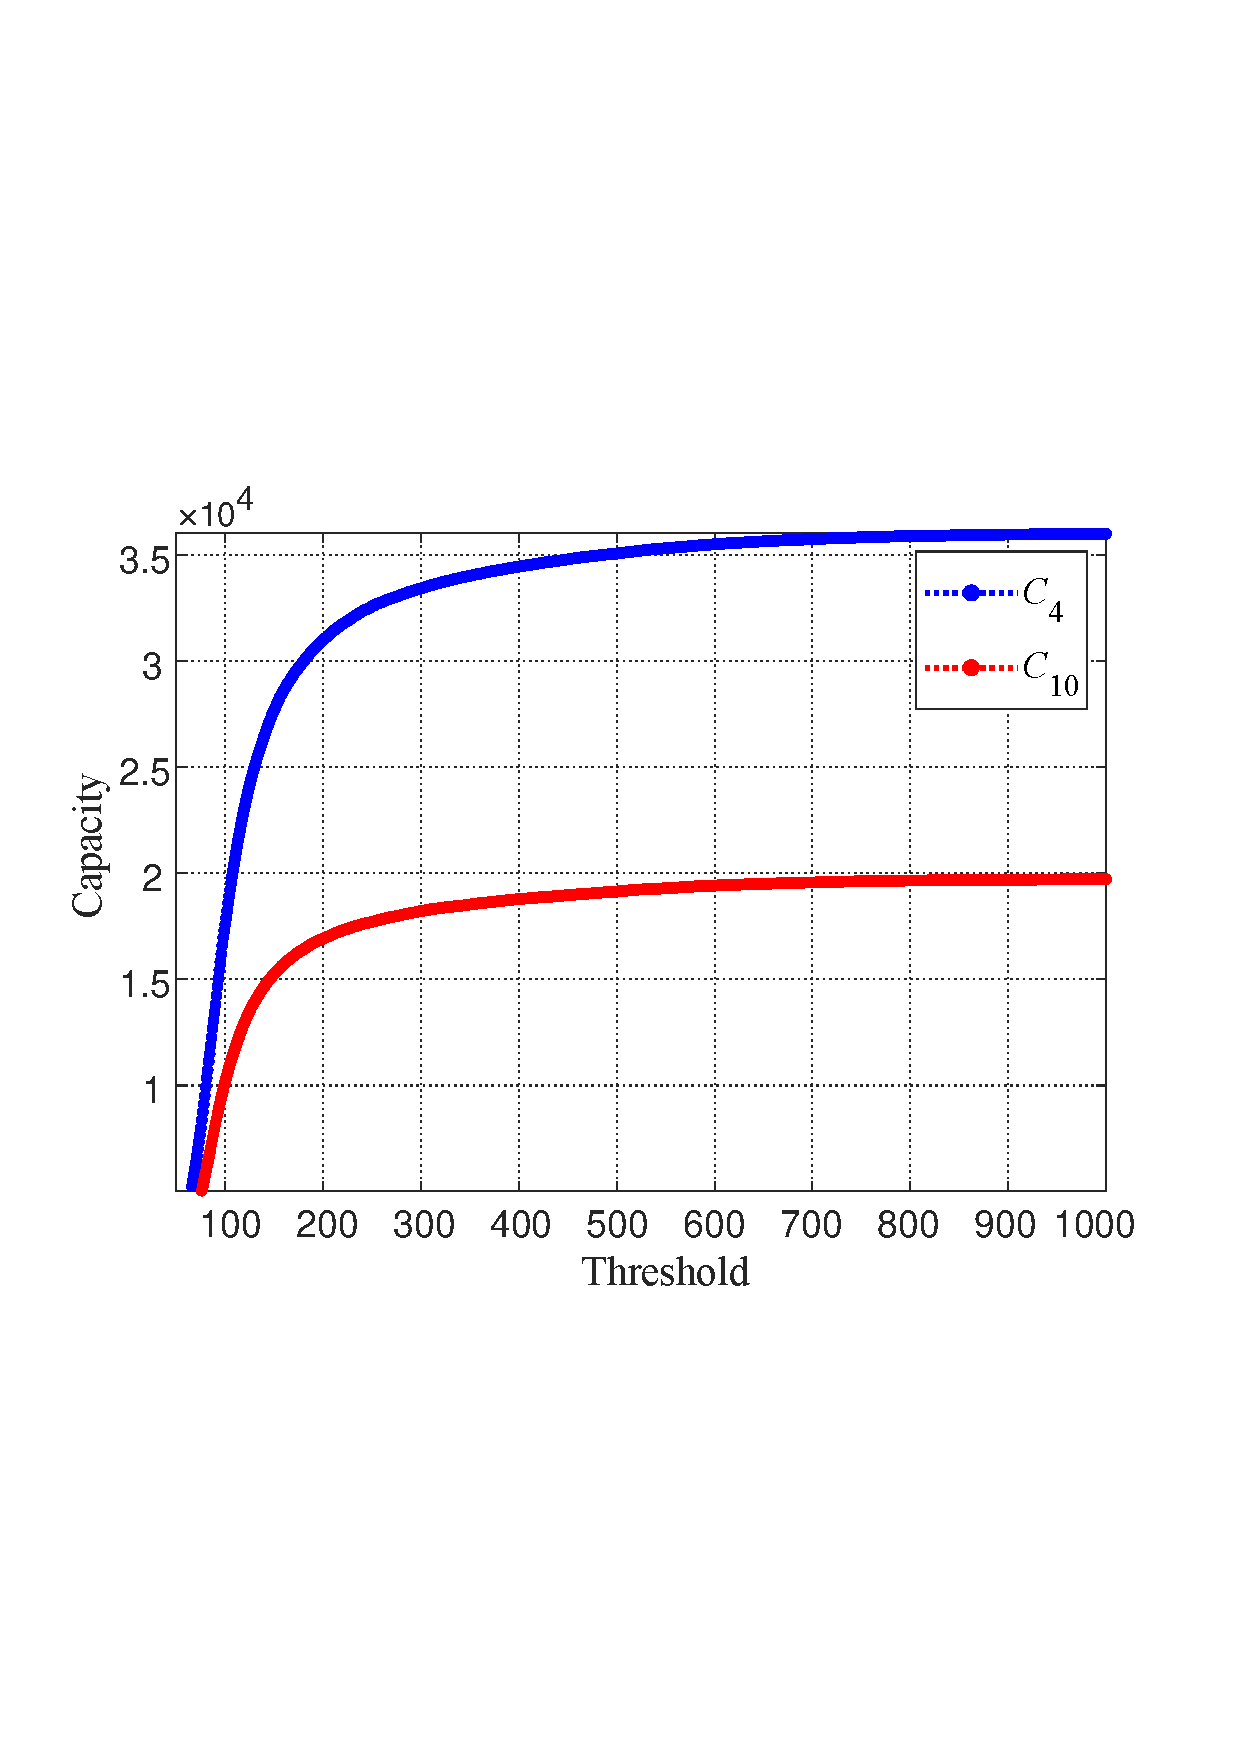
\includegraphics[width=1\textwidth]{figures/CapLena.pdf}
    \end{minipage}
}
\qquad
\subfigure[]{
    \begin{minipage}[t]{0.46\linewidth}
    \centering
    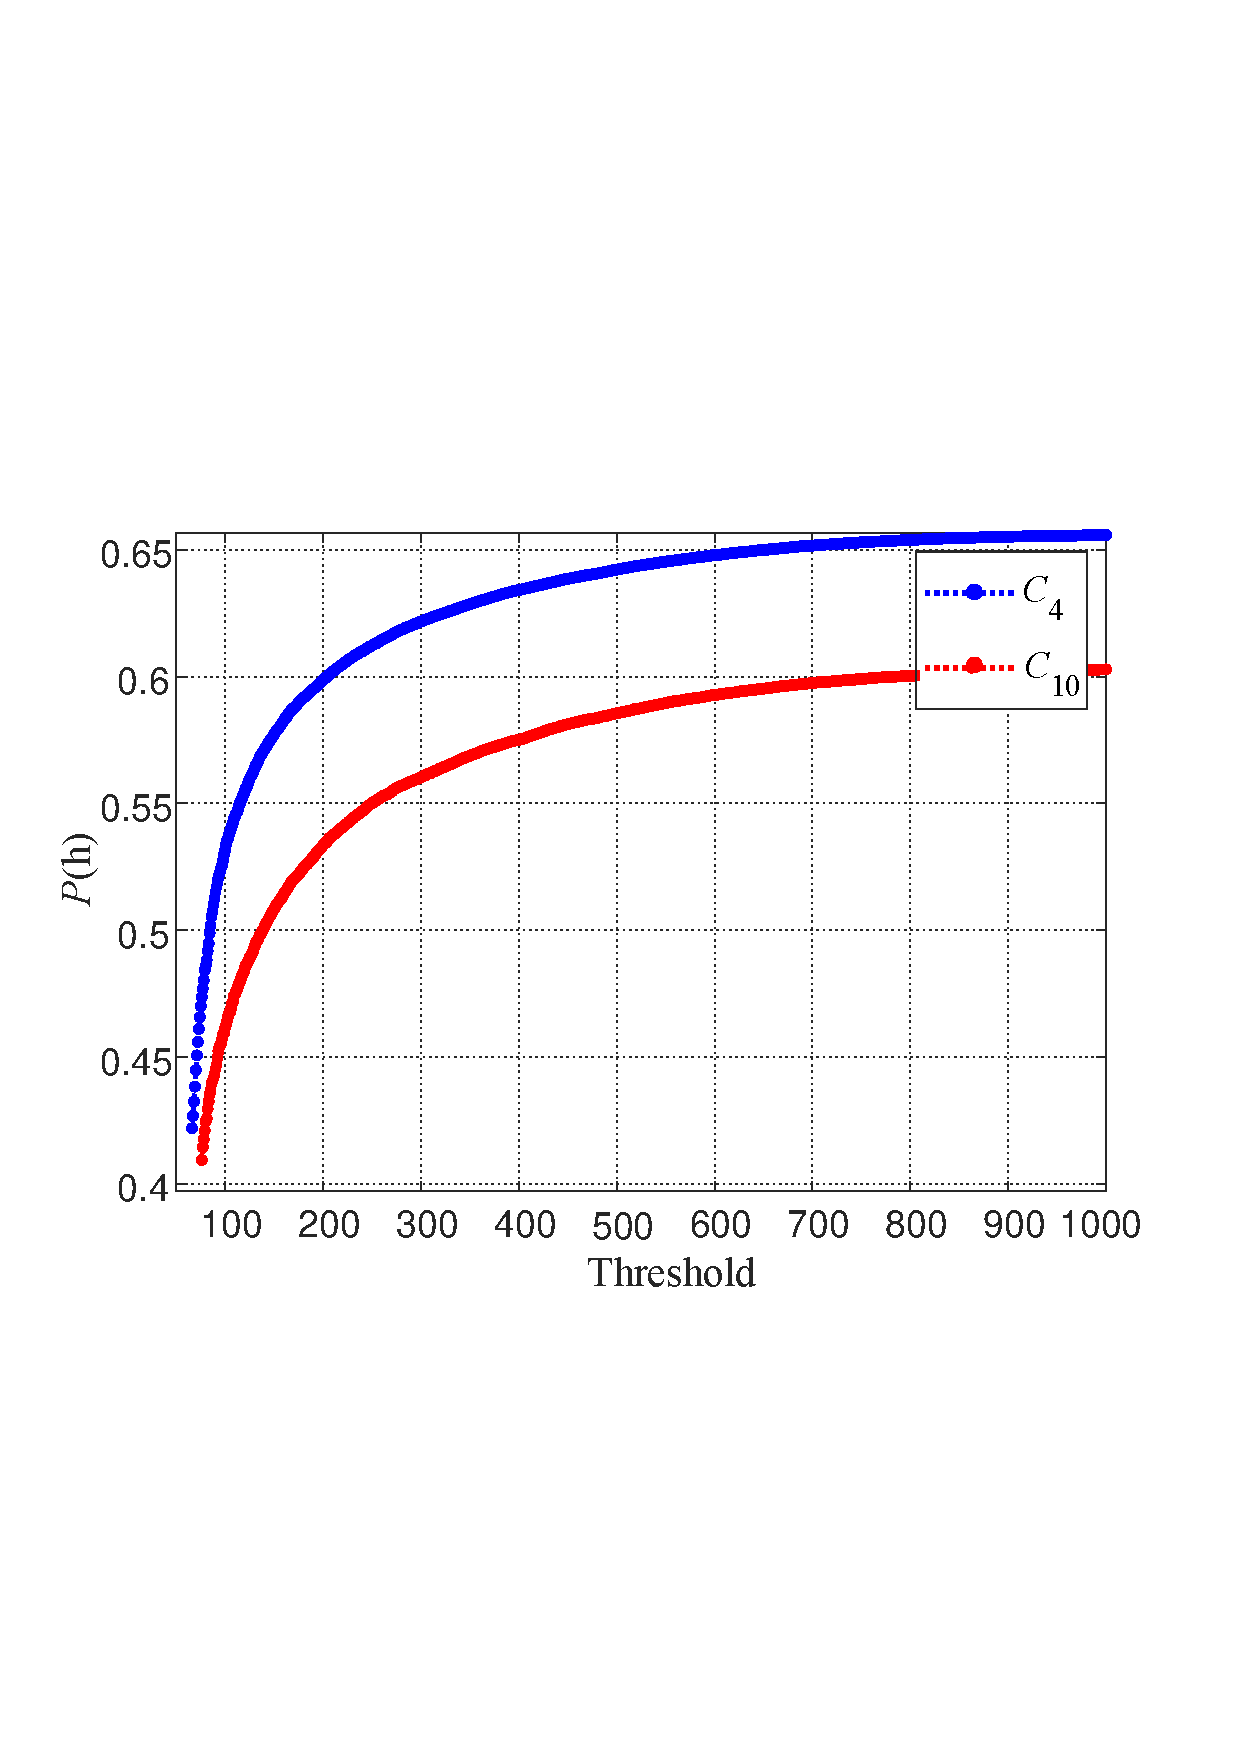
\includegraphics[width=1\textwidth]{figures/thPropLena.pdf}
    \end{minipage}
}
\centering
\caption{Eval of Lena.}
\label{Fig.Eval}
\end{figure*}
\begin{figure*}
\centering
    \begin{minipage}[t]{0.5\linewidth}
    \centering
    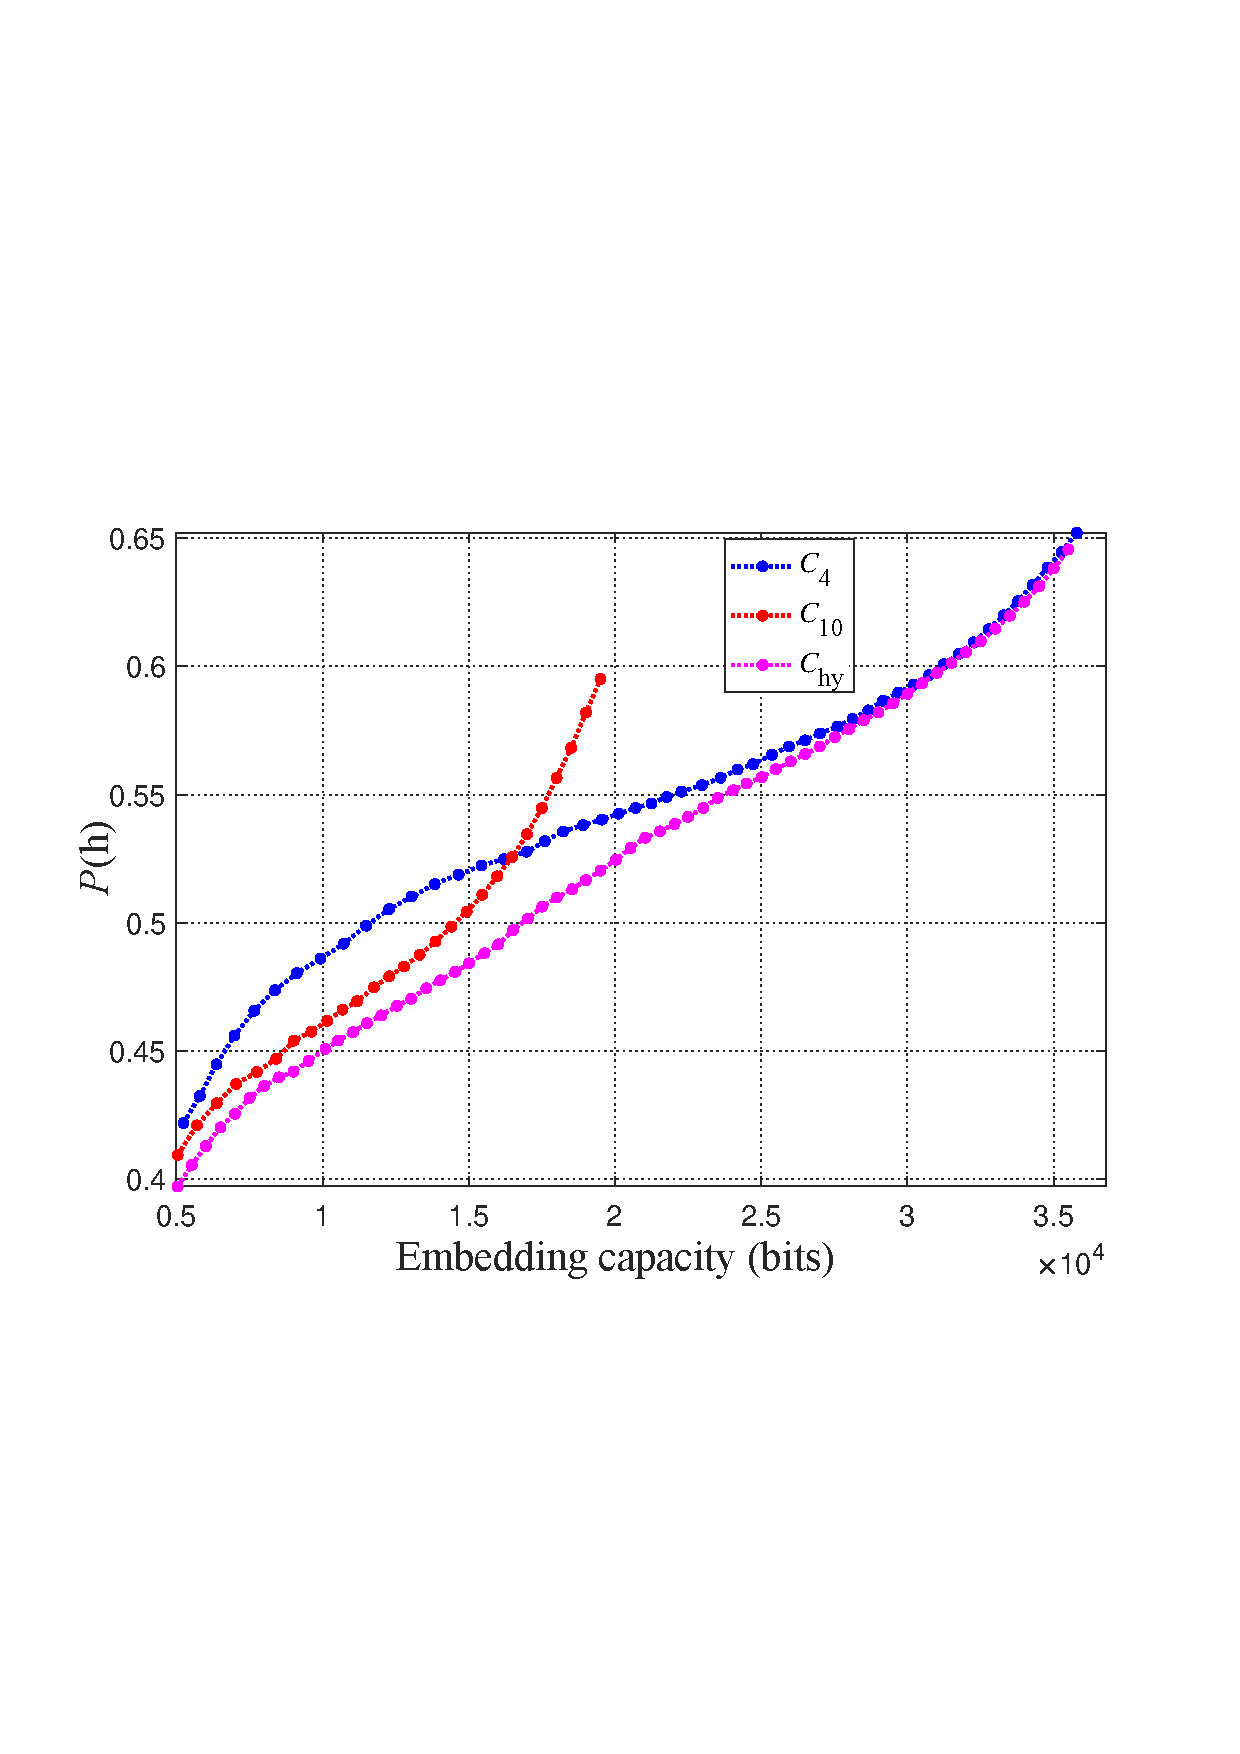
\includegraphics[width=1\textwidth]{figures/PropLenaNoT.pdf}
    \end{minipage}
\centering
\caption{Eval of Lena.}
\label{Fig.Eval0}
\end{figure*}

\begin{figure*}
\centering
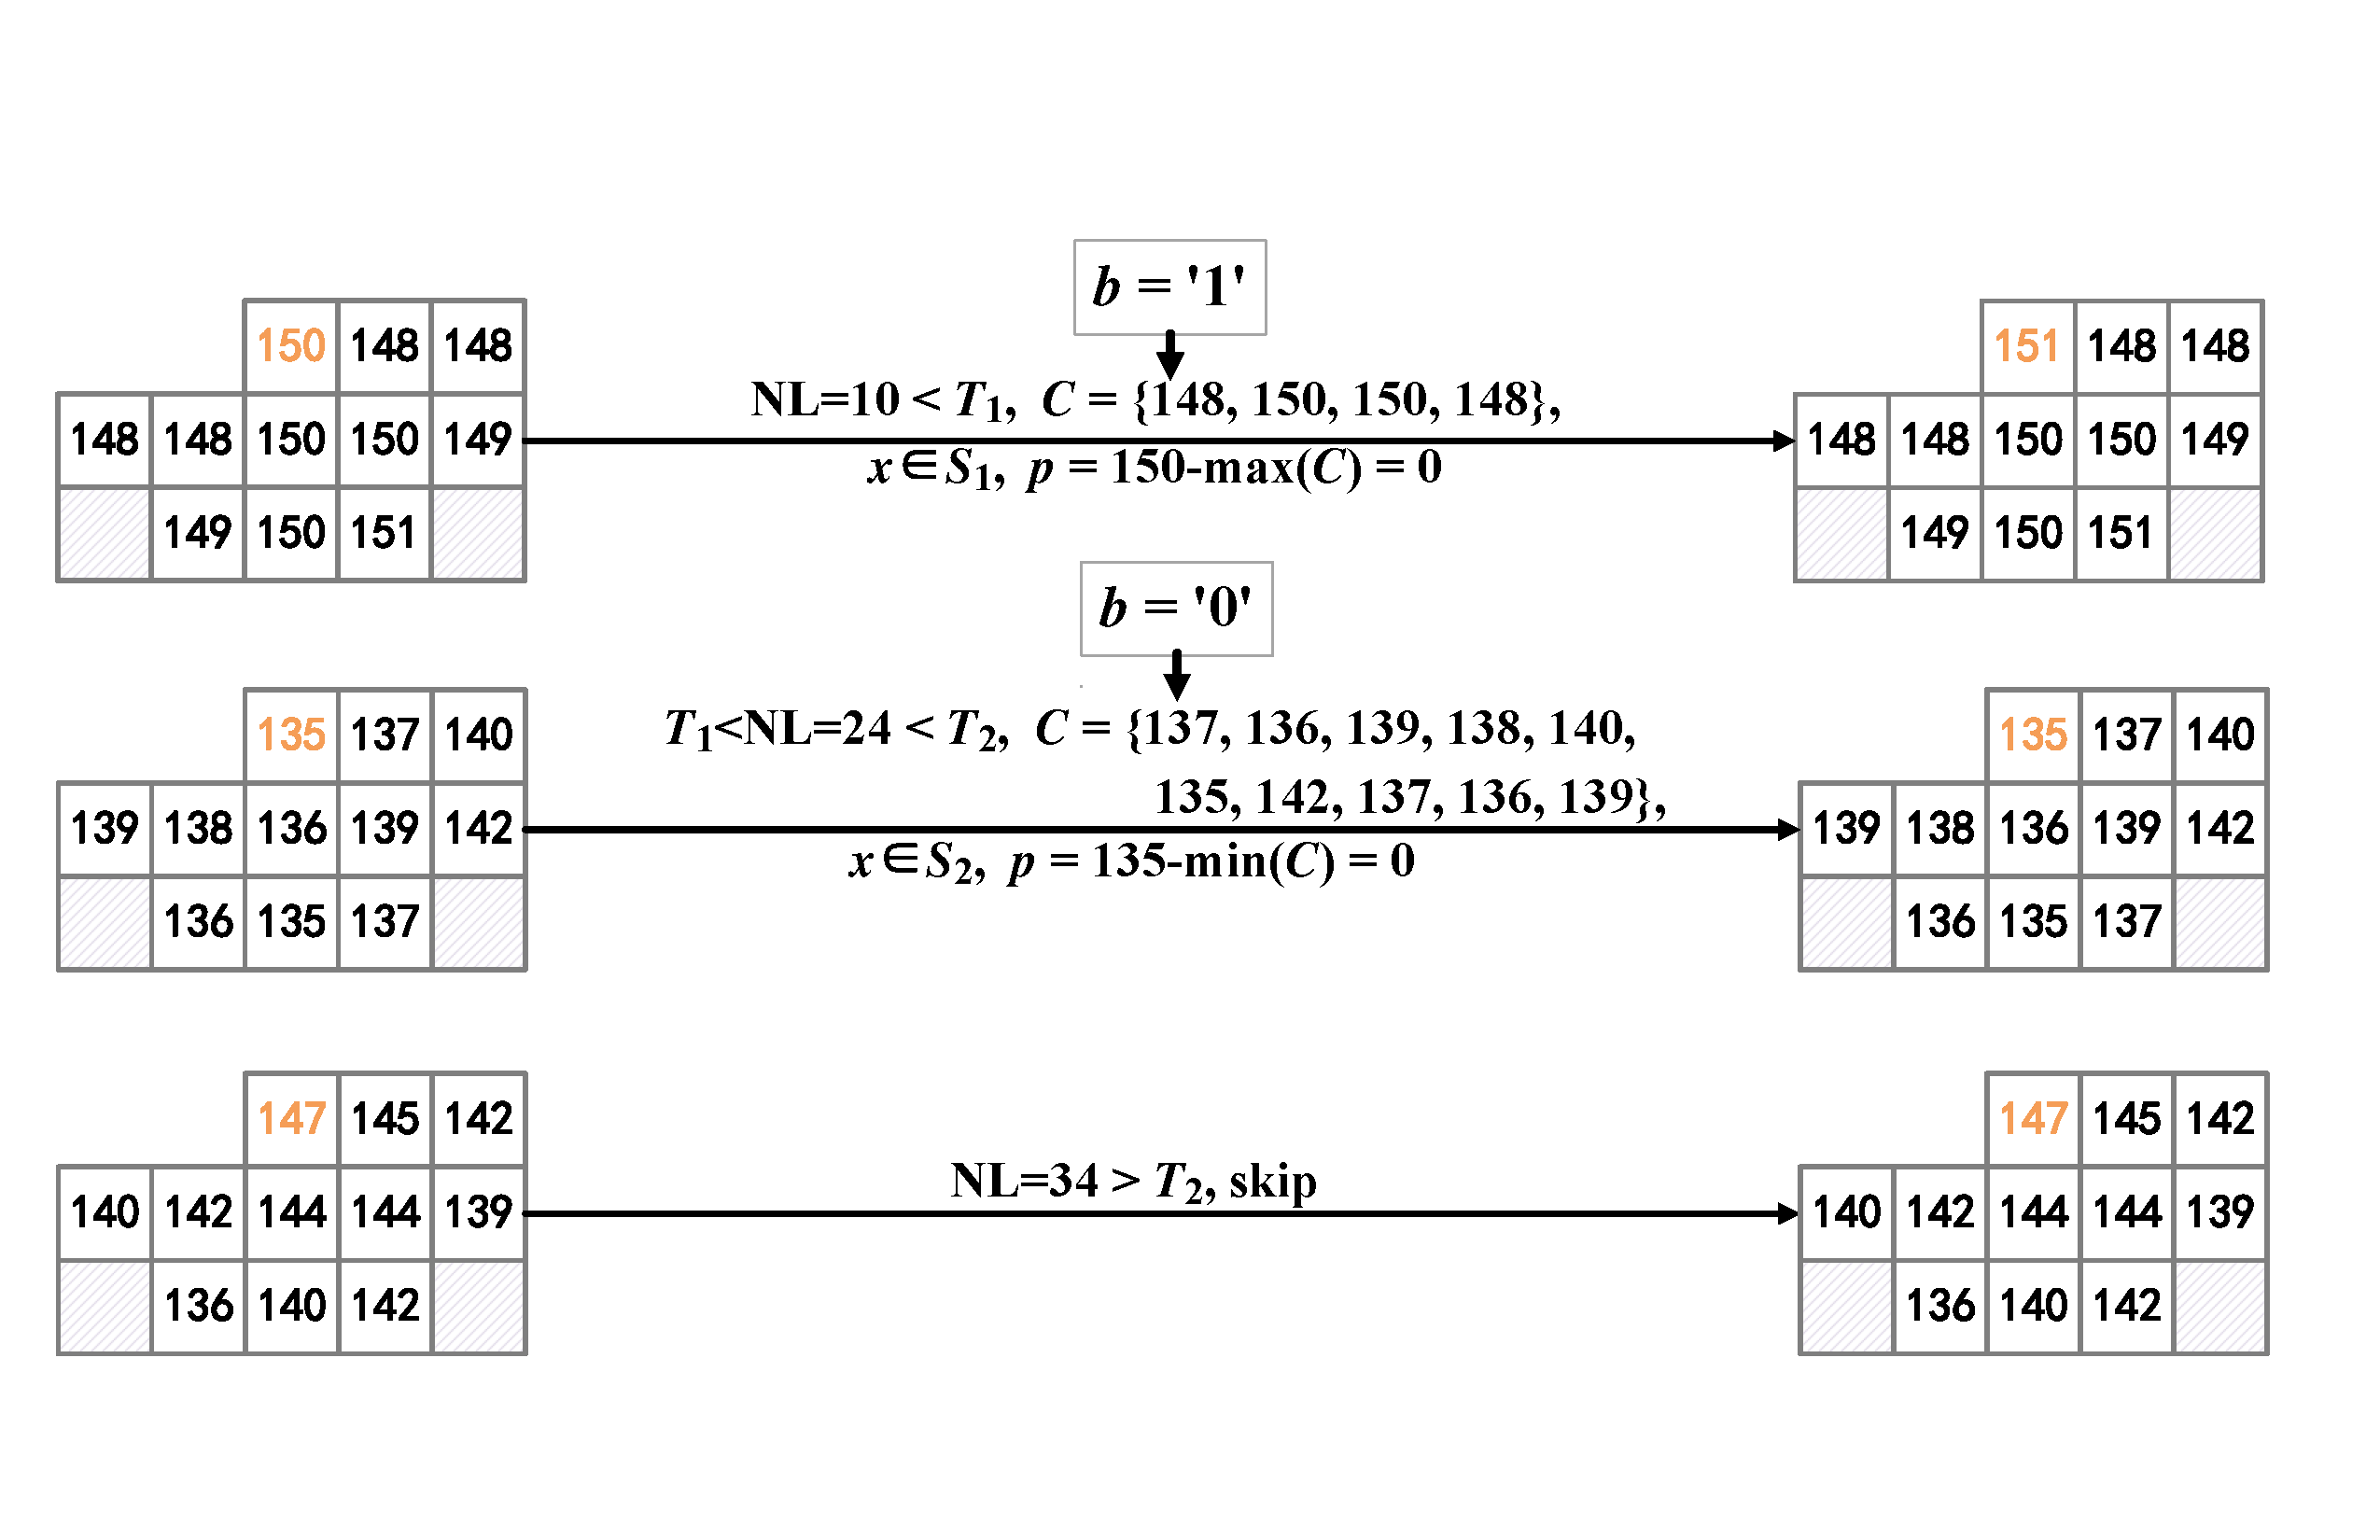
\includegraphics[width=0.7\textwidth]{figures/EmbedwithTh.pdf}
\centering
\caption{Example.}
\label{Fig.EmbedExample}
\end{figure*}

\begin{figure*}
\centering
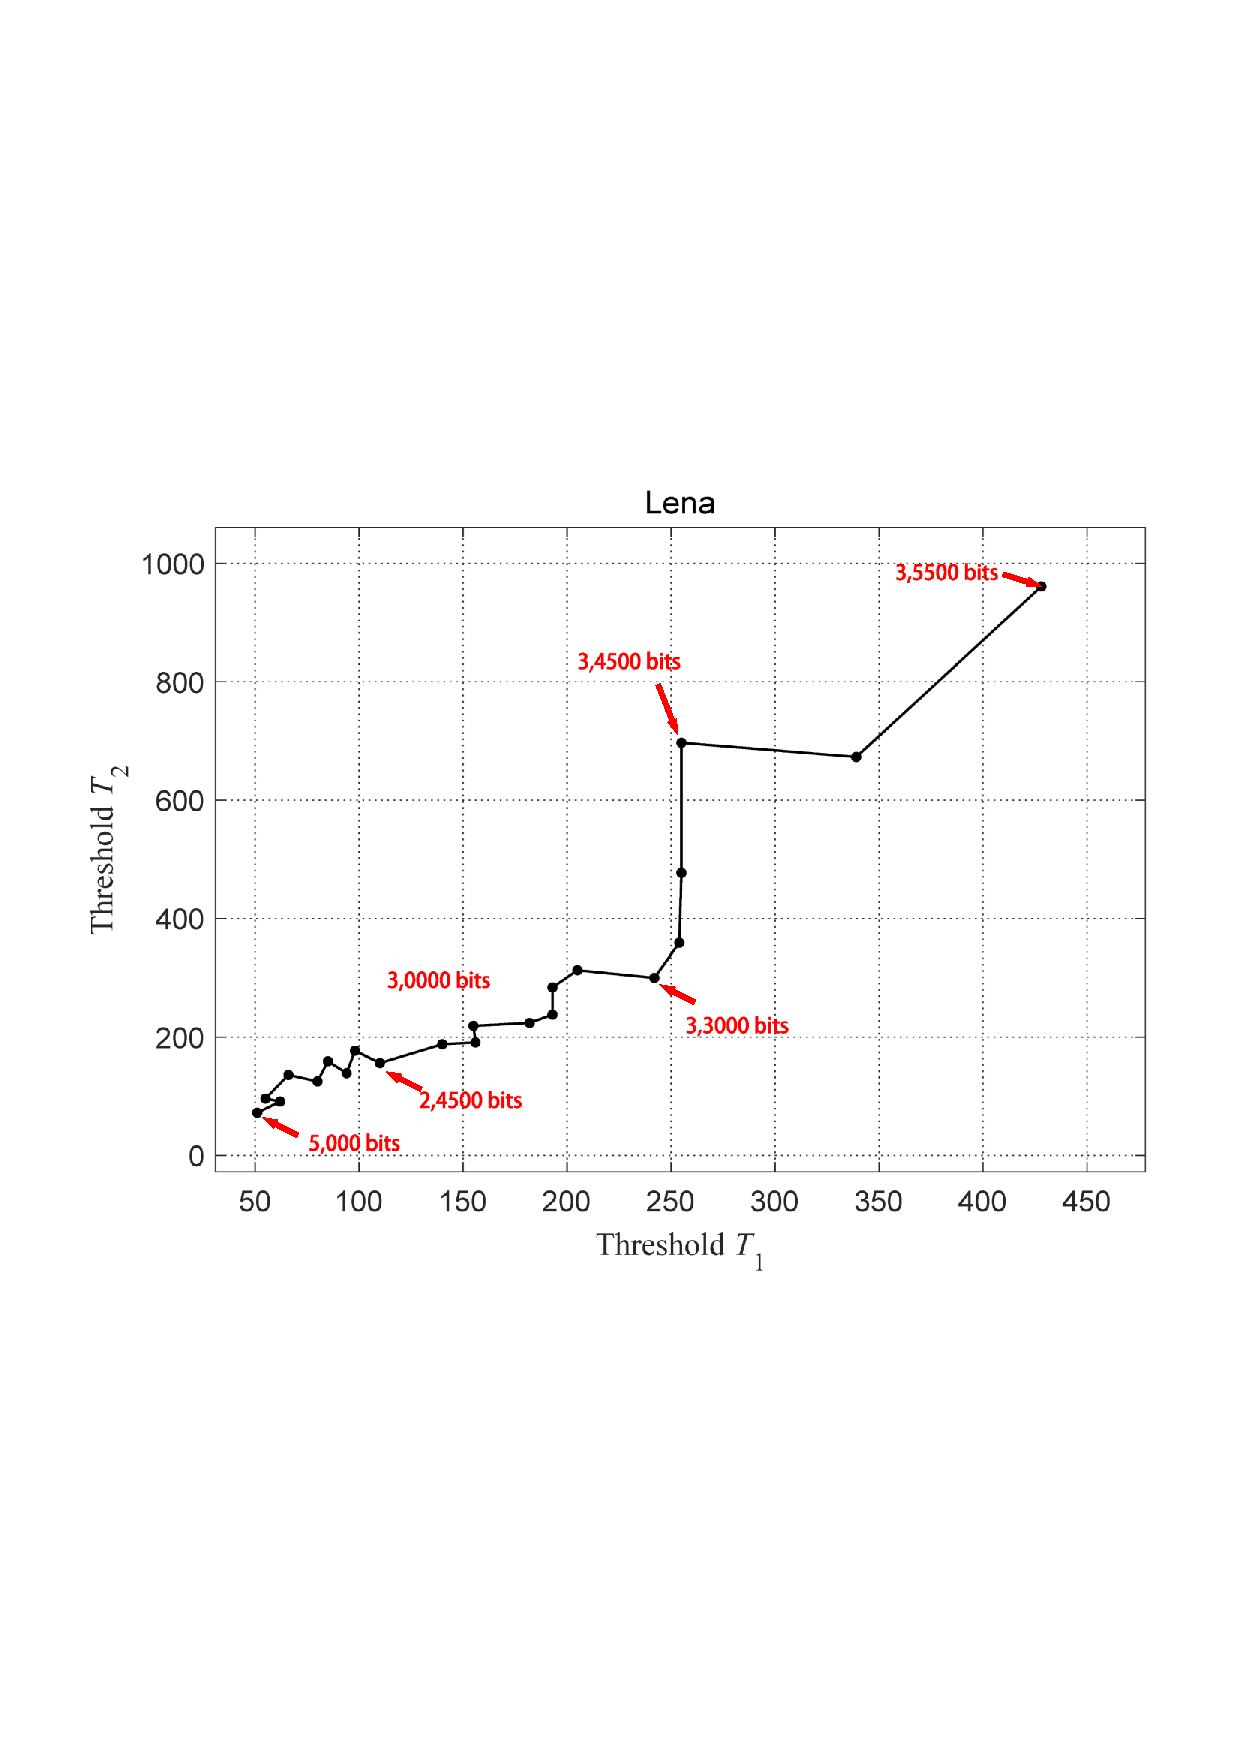
\includegraphics[width=0.5\textwidth]{figures/Thresholds.pdf}
\centering
\caption{Thresholds.}
\label{Fig.Thresholds}
\end{figure*}

In addition, more sizes of context pixels can be used for further improvement of the embedding performance. Based on Fig. \ref{Fig.Context3}, four cases with different sizes of context pixels are tested here, and corresponding experimental results on images of Lena and Baboon are shown in Fig. \ref{fig:size}. Specifically, the first case only takes $C_1$ into consideration, and it is shown as $C_1$ in Fig. \ref{fig:size}. The second case employs two sizes of context pixels with $C_1$ and $C_2$ for prediction, and the corresponding result is shown in Fig. \ref{fig:size} as $C_{12}$. Similarly, $C_{123}$ represent the case that $C_1, C_2$ and $C_3$ are used, and $C_{1234}$ represent the case that $C_1, C_2, C_3$ and $C_4$ are used for prediction. Obviously, by employing more different sizes of context pixels for prediction, the embedding performance is improved. And the best embedding performance is obtained in the case of $C_{1234}$. However, since the embedding results of $C_{123}$ is very close to the case of $C_{1234}$, while it is more time-saving, we finally take three different sizes of context pixels as $C_1, C_2$ and $C_3$ for the prediction of the proposed method. Accordingly, three thresholds $\{t_1, t_2, t_3\}$ are needed for the implementation of the proposed method, and specific procedures of the embedding and the extraction process are given in the next subsection.


\begin{figure*}
\centering
\subfigure{
\begin{minipage}[t]{0.4\linewidth}
\centering
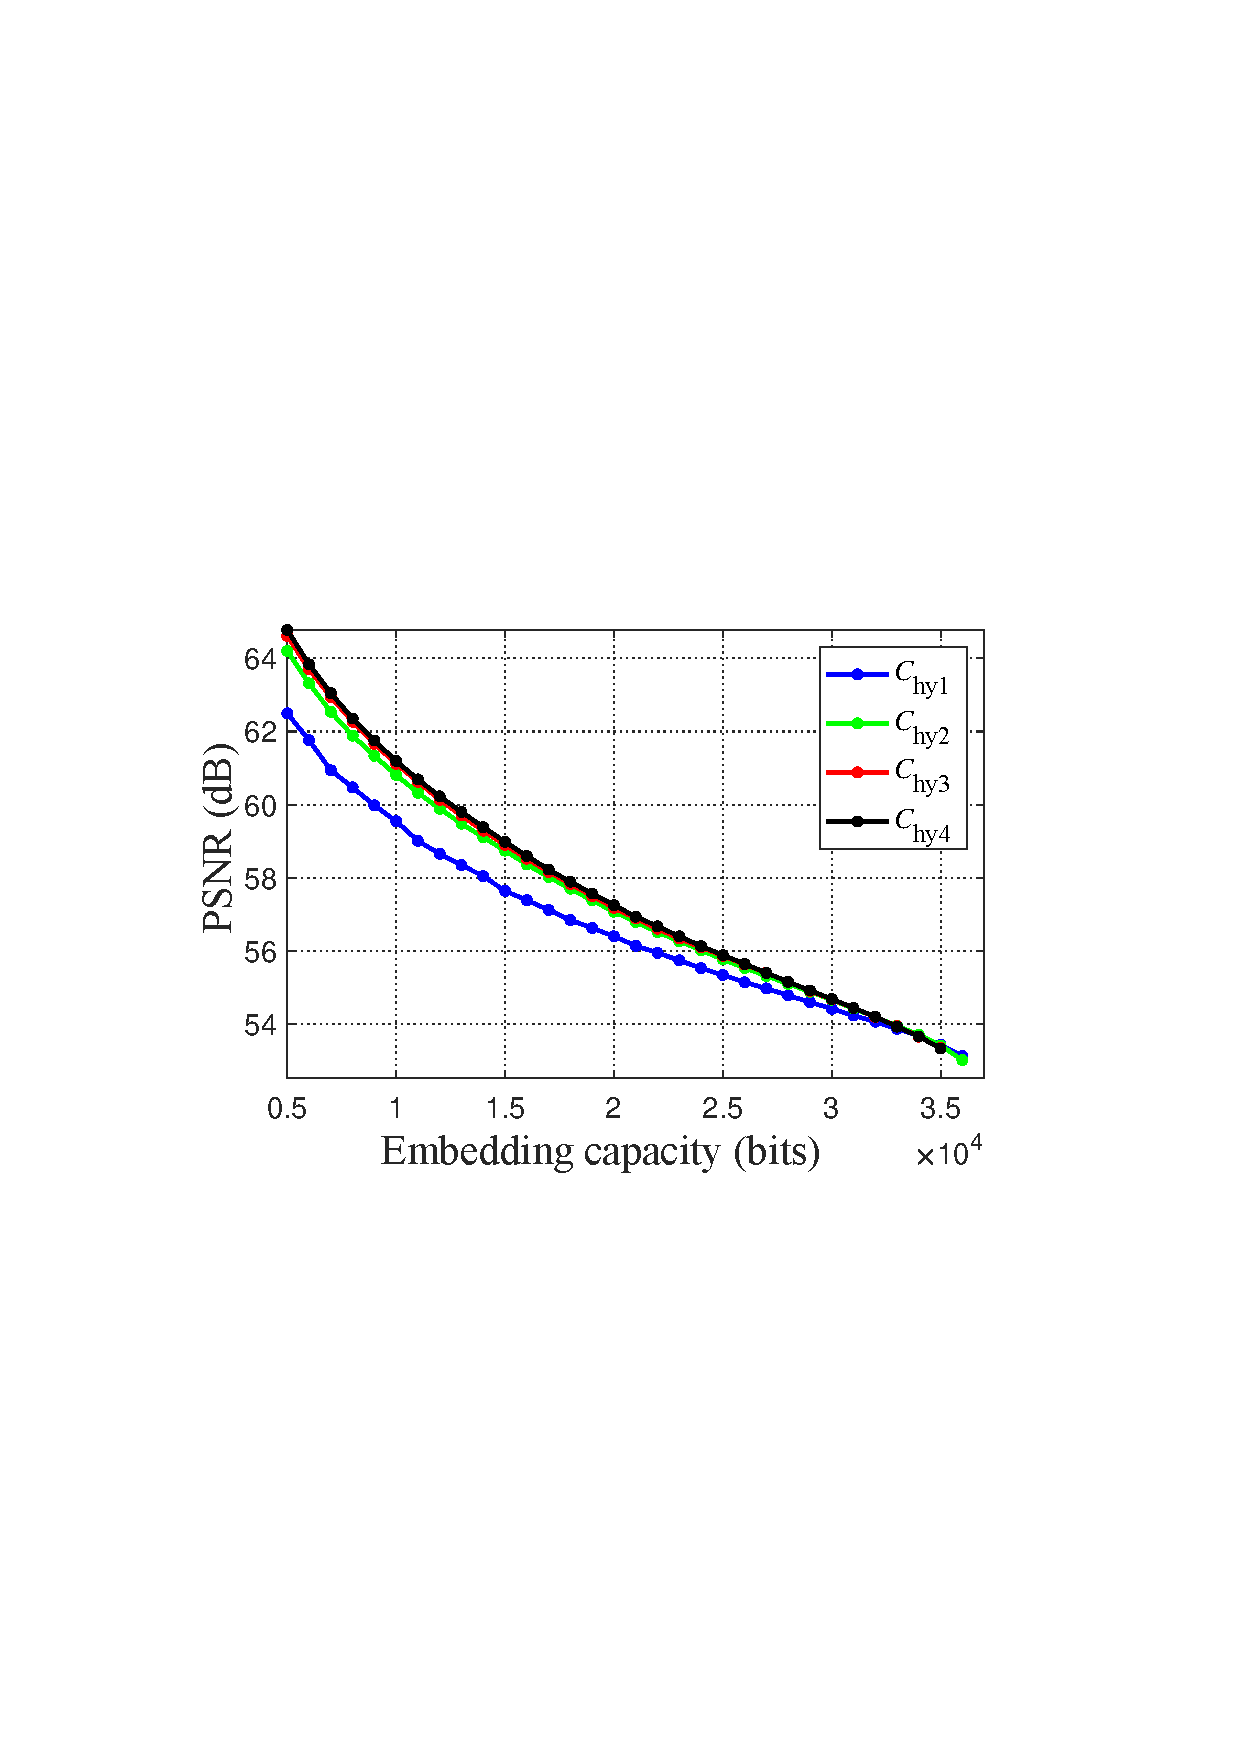
\includegraphics[width=1\textwidth]{figures/Result/size/Lena.pdf}
\end{minipage}
}
\qquad
\subfigure{
\begin{minipage}[t]{0.412\linewidth}
\centering
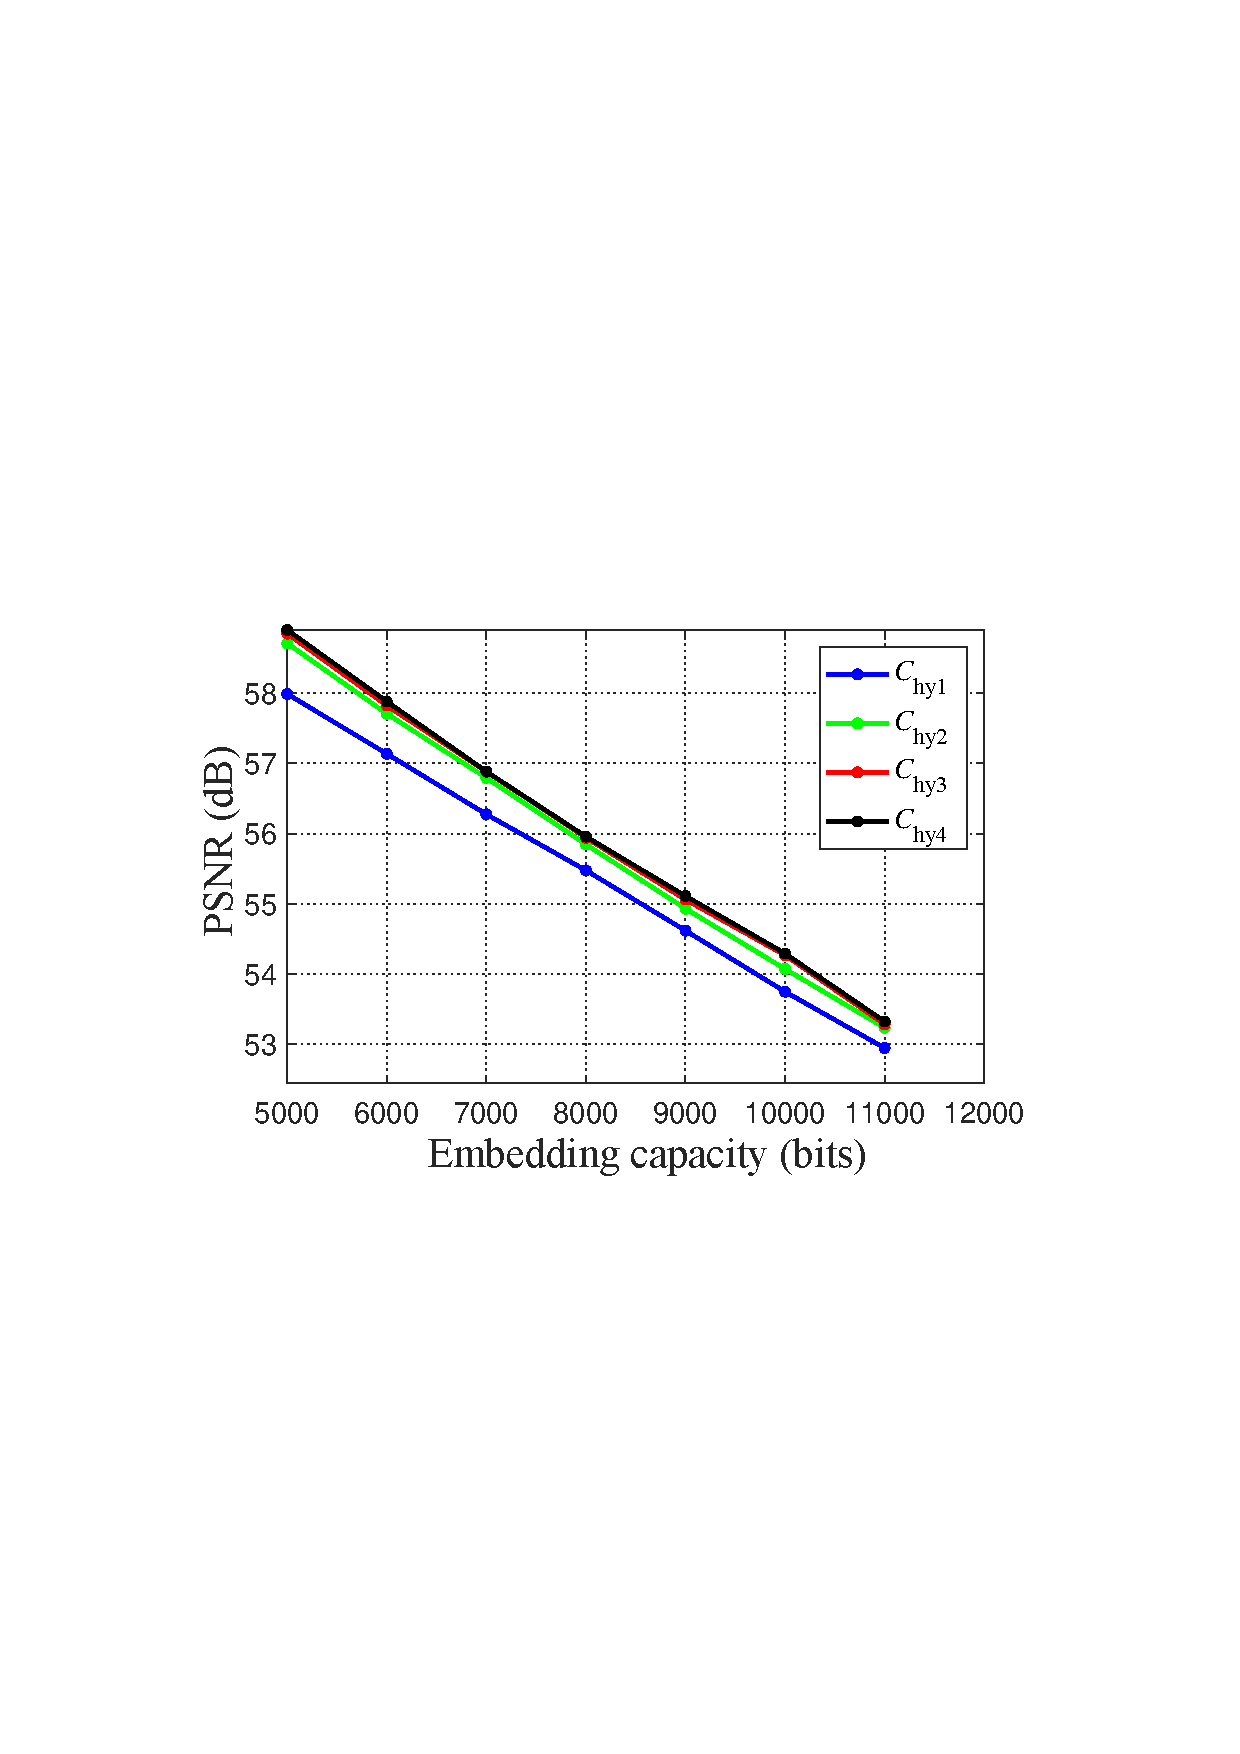
\includegraphics[width=1\textwidth]{figures/Result/size/Baboon.pdf}
\end{minipage}
}
\centering
\caption{size.}
\label{fig:size}       % Give a unique label
\end{figure*}


\subsection{Data Embedding and Extraction Procedures}\label{sec:3.3}
For the data embedding process, it is conducted by following steps. First, a location map $ \rm LM$ is constructed to avoid the overflow and underflow problem. For the $i$-th cover pixel $x_i$, if $x_i$ equals 0 or $255$, we set ${\rm LM}(i) = 1$. Otherwise, ${\rm LM}(i) = 0$. And it is further compressed by arithmetic coding to reduce its length. Then, for the cover image, pixels valued $255$ are modified to $254$ and pixels valued $0$ are changed to $1$. Next, the local complexity of all the pixels are calculated by the context region based on $C_3$. In addition, for a certain value of the three thresholds $(t_1, t_2, t_3)$, the cover pixels are classified into four classes based on their local complexity, and pixels in different classes are predicted based on different number of context pixels as described in Section \ref{sec:3.2}. Note that, the embedding procedures presented in Section \ref{sec:2} are used here except for the prediction of cover pixels. Accordingly, the data embedding process is performed in a pixelwise way until all the secret data is embedded into the cover image, and the position of the last pixel used for embedding is recorded as $k_{\rm end}$. Moreover, for blind extraction, some auxiliary information also should be embedded, including
\begin{itemize}
  \item the local complexity thresholds $t_1$, $t_2$ and $t_3$ ($11 \times 3 = 33$ bits),
  \item the position of the last pixel used for embedding $k_{\rm end}$ (18 bits),
  \item the length of the compressed location map $L$ (18 bits),
  \item the compressed location map.
\end{itemize}
The auxiliary information is embedded into the least significant bits (LSB) of the first $69 + L$ pixels in the first row. And the original LSBs of these pixels are embedded into the cover image together with the payload.
Note that, for a fixed payload, the optimal thresholds used for embedding are determined by exhaustively search.

The extraction process is conducted based on reverse procedures of the embedding process, and specific procedures are omitted for simplicity.

%As for the extraction process, it is conducted through reverse procedures. First, auxiliary information is obtained by reading LSBs of first $69 + L$ pixels in the first row. Then, the local complexity of marked pixels is computed in the same way with the embedding process. Next, for a marked pixel, based on the extracted three complexity thresholds $(t_1, t_2, t_3)$, the secret data bit can be extracted based on the same number of context pixels used in the embedding phase, and the pixel can be recovered. Accordingly, all the secret data bits can be extracted in the reverse order to the embedding process, and the cover pixels can be recovered at the same time. Moreover, based on the extracted compressed location map, pixels at the locations with ${\rm LM}(i) = 1$ are recovered to its original values, and the LSBs of the first $69 + L$ pixels in the first row are recovered based on the extracted payload. Finally, the secret data is extracted and the original image is recovered.


%----------------------------------------------------------------------------------------
\section{Experimental Results}\label{sec:4}
% N \in {1, 2, 3, 4}, N=4 been chosen,
In this section, in order to demonstrate the effectiveness of the proposed RDH method, it is compared with three state-of-the-art PVO-based methods. They are the methods of Peng \emph{et al.} \cite{Peng2014IPVO}, Ou \emph{et al.} \cite{Ou2014PVOk} and Qu \emph{et al.} \cite{Qu2015PPVO}. All the experiments are implemented based on Matlab with the version of 2018a on a tower server (SUPERMICRO LT-7038AX). And, it is worth mentioning that, for a given cover image with a fixed payload, the proposed method can complete the embedding process within four seconds.

The experiments are conducted based on eight standard $512 \times 512$ sized gray-scale images, including Lena, Baboon, Airplane, Barabra, Lake, Boat, Peppers and Elaine. And the corresponding comparison results are shown with capacity-distortion curves in Fig. \ref{fig:size}. Specifically, the embedding capacity increases from 5,000 bits to the largest capacity with a step of 1,000 bits. According to this figure, it is obvious that the embedding performance of the proposed method is superior to other three PVO-based methods. Moreover, the comparison results on PSNR values for fixed embedding capacities with 10,000 bits and 20,000 bits are given in Table~\ref{tab:10000bits} and Table~\ref{tab:20000bits}. Besides, the optimal parameters $(t_1^*, t_2^*, t_3^*)$ of proposed method on different images are also listed in the tables. Note that, for a fixed embedding capacity, the optimal thresholds for different images are different from each other. However, since the computational complexity of the proposed method is acceptable, exhaustive search is adopted for better embedding performance.

As mentioned above, the improved PVO-based RDH proposed by Peng \emph{et al.} \cite{Peng2014IPVO} achieved performance enhancement upon the original PVO-based RDH method \cite{Li2013PVO}. The cover image is first divided into non-overlapping blocks with equal size, and then secret data is embedded into the largest and smallest pixels of each block. Compared with the original PVO-based RDH, in \cite{Peng2014IPVO}, more smooth blocks are utilized for data embedding by taking the pixel values as well as their locations into consideration. However, its embedding performance can be further improved. According to the comparison results shown in Fig. \ref{fig:size}, the proposed method outperforms it on all the test images. In addition, based on Table~\ref{tab:10000bits} and Table~\ref{tab:20000bits}, the proposed method obtains an PSNR increase of 0.90 dB and 0.99 dB for the embedding capacity of 10,000 bits and 20,000 bits, respectively.

The PVO-$k$ RDH method proposed by Ou \emph{et al.} \cite{Qu2015PPVO} is another improved method of the original PVO \cite{Li2013PVO}, which aims to make full use of smooth blocks as well. In this method, the embedding performance is optimized by combining PVO-$1$ with PVO-$2$. Although better embedding performance is achieved compared with the improved PVO-based method, there still has much room for improvements. According to Table~\ref{tab:10000bits} and Table~\ref{tab:20000bits}, the proposed method outperforms this method with 0.63 dB and 0.78 dB for the embedding capacity of 10,000 bits and 20,000 bits, respectively.

The PPVO RDH method proposed by Qu \emph{et al.} \cite{Qu2015PPVO} is quiet different from traditional PVO-based RDH methods \cite{Li2013PVO,Peng2014IPVO,Ou2014PVOk}. They proposed to perform prediction for each pixel to enlarge the embedding capacity as well as gain better embedding performance. Besides, the optimal number of context pixels is obtained by implementing the embedding process for 15 times to test $n$ from 1 to 15, and the marked image with highest PSNR is considered as the final embedding result. The embedding performance of PPVO is superior to previous PVO-based RDH methods. However, by choosing more suitable context pixels as well as make full use of the difference of pixel local complexity, the embedding performance is further improved by the proposed method. Specifically, based on Table~\ref{tab:10000bits} and Table~\ref{tab:20000bits}, the proposed method gets an increase of PSNR by 0.57 dB for an embedding performance of 10,000 bits and 0.44 dB for an embedding performance of 20,000 bits.


\begin{figure*}
\centering
\subfigure{
\begin{minipage}[t]{0.415\linewidth}
\centering
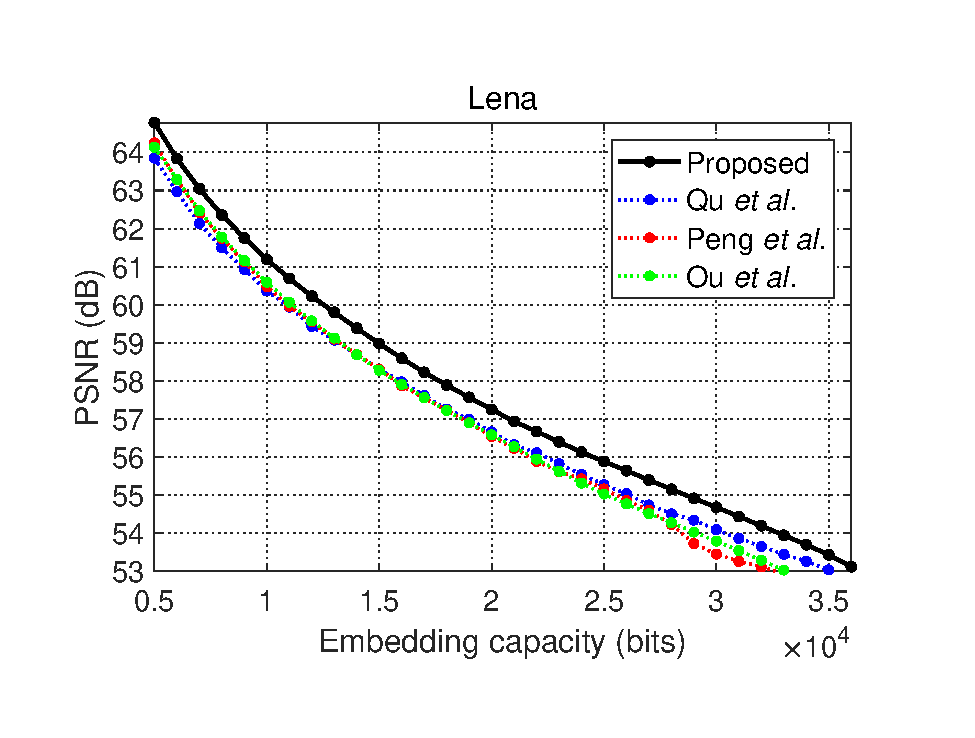
\includegraphics[width=1\textwidth]{figures/Result/capacity/Lena.pdf}
\end{minipage}
}
\subfigure{
\begin{minipage}[t]{0.43\linewidth}
\centering
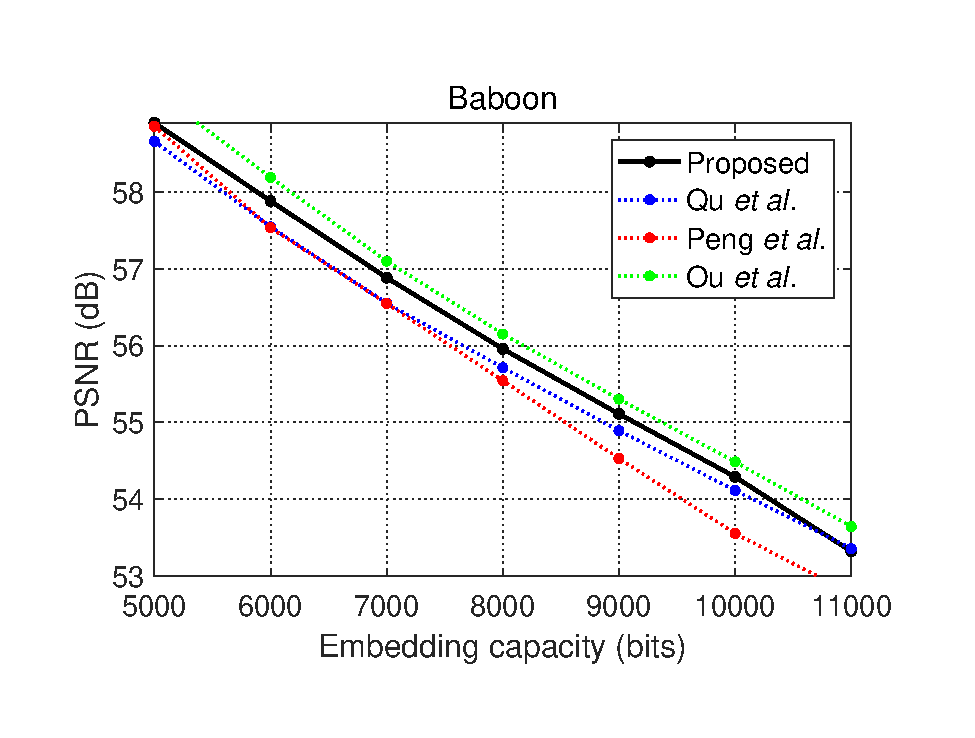
\includegraphics[width=1\textwidth]{figures/Result/capacity/Baboon.pdf}
\end{minipage}
}

\subfigure{
\begin{minipage}[t]{0.415\linewidth}
\centering
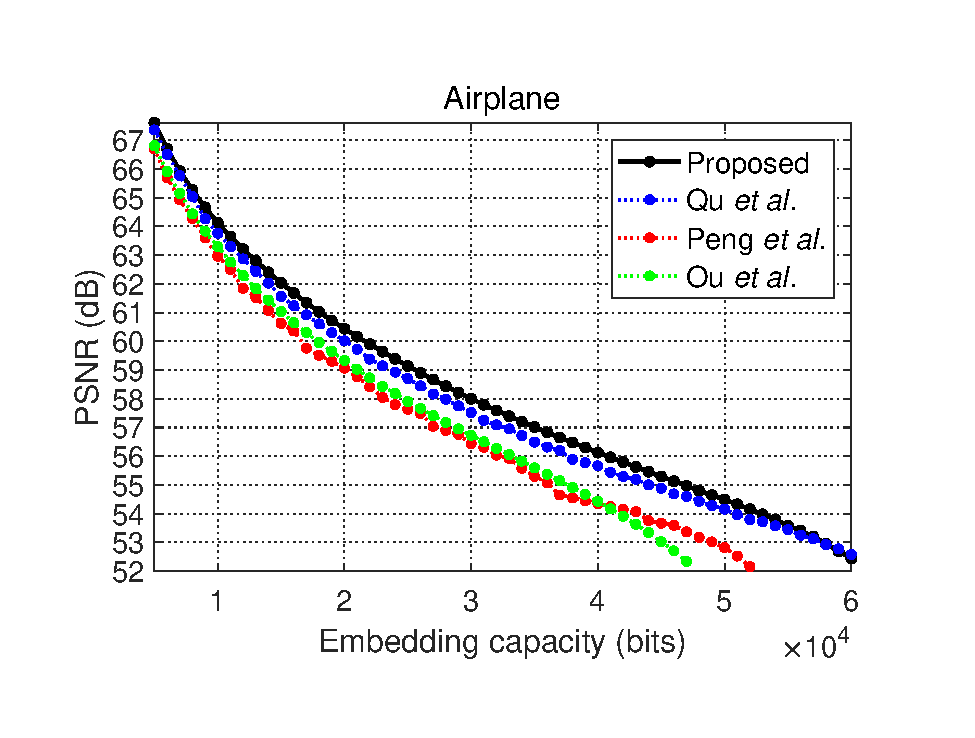
\includegraphics[width=1\textwidth]{figures/Result/capacity/Airplane.pdf}
\end{minipage}
}
\subfigure{
\begin{minipage}[t]{0.415\linewidth}
\centering
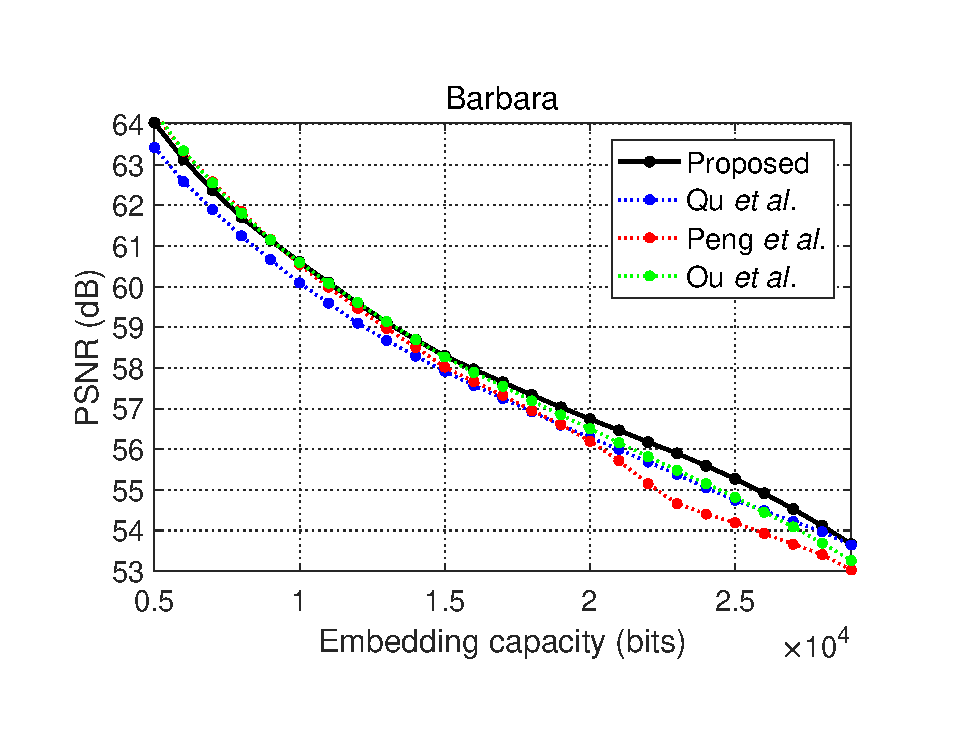
\includegraphics[width=1\textwidth]{figures/Result/capacity/Barbara.pdf}
\end{minipage}
}

\subfigure{
\begin{minipage}[t]{0.415\linewidth}
\centering
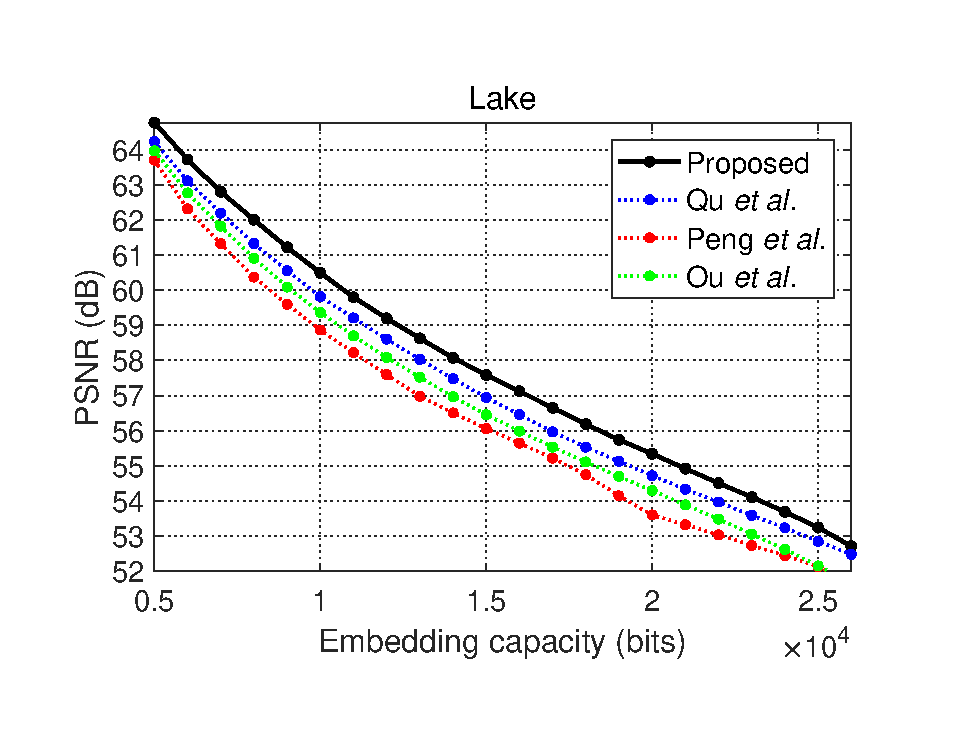
\includegraphics[width=1\textwidth]{figures/Result/capacity/Lake.pdf}
\end{minipage}
}
\subfigure{
\begin{minipage}[t]{0.42\linewidth}
\centering
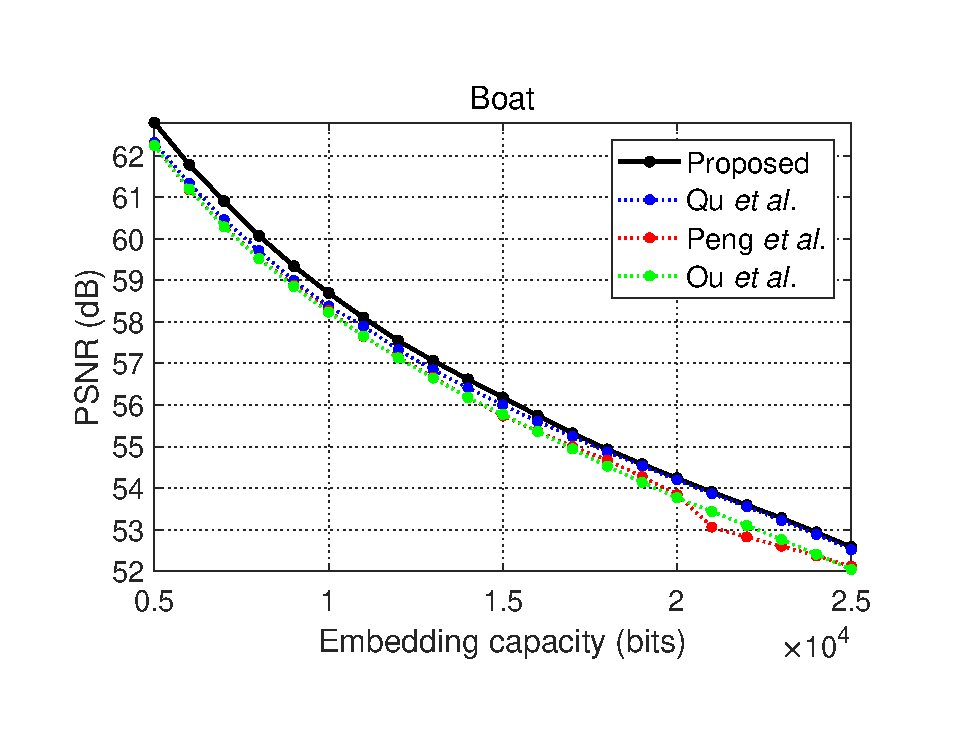
\includegraphics[width=1\textwidth]{figures/Result/capacity/Boat.pdf}
\end{minipage}
}

\subfigure{
\begin{minipage}[t]{0.415\linewidth}
\centering
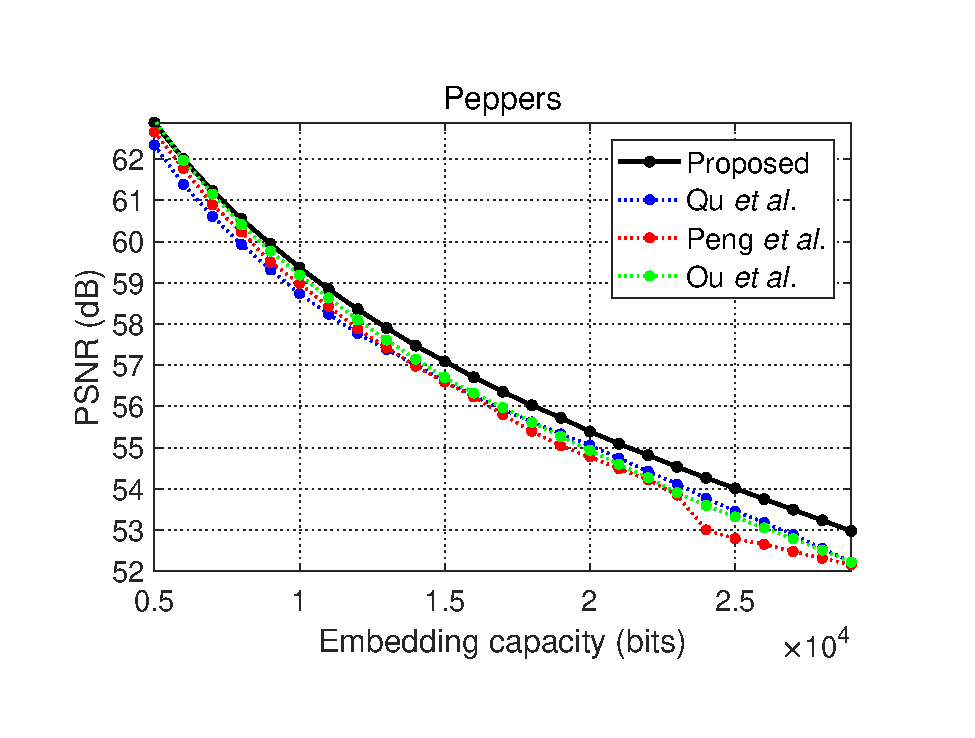
\includegraphics[width=1\textwidth]{figures/Result/capacity/Peppers.pdf}
\end{minipage}
}
\subfigure{
\begin{minipage}[t]{0.415\linewidth}
\centering
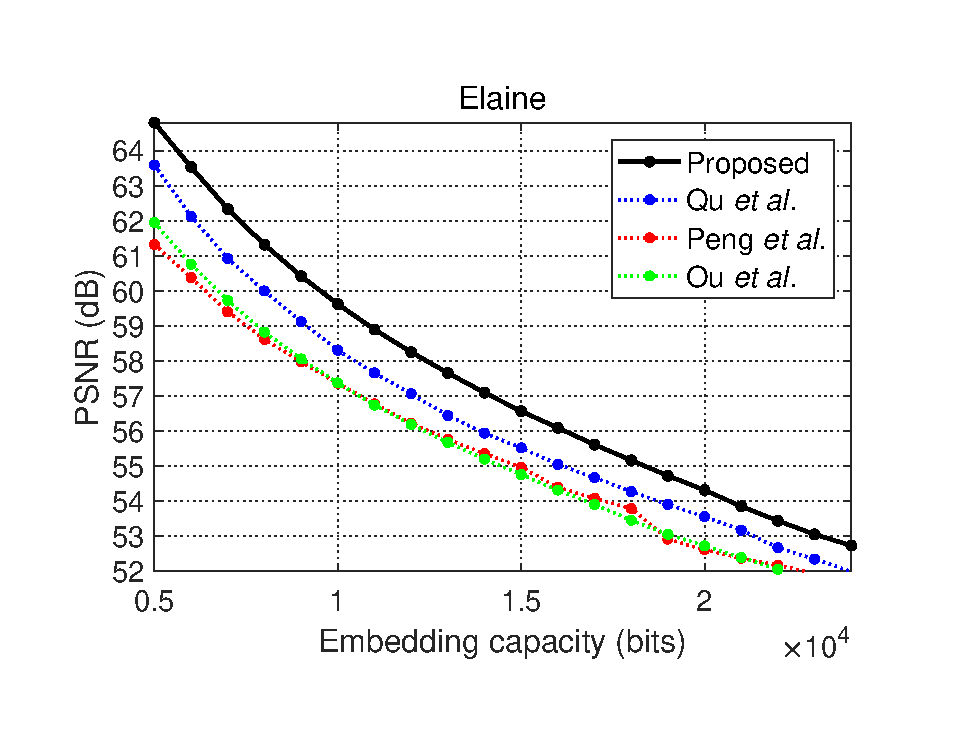
\includegraphics[width=1\textwidth]{figures/Result/capacity/Elaine.pdf}
\end{minipage}
}
\centering
\caption{capacity.}
\label{fig:capacity}       % Give a unique label
\end{figure*}

\begin{table*}
\scriptsize
\centering
\caption{Comparison of PSNR (dB) among the proposed method and the PVO-based methods of Peng \emph{et al.} \cite{Peng2014IPVO}, Ou \emph{et al.} \cite{Ou2014PVOk} and Qu \emph{et al.} \cite{Qu2015PPVO}. The embedding capacity is 10,000 bits. The optimal parameters of the proposed method are also listed.}
\setlength{\tabcolsep}{3mm}{
\begin{tabular}{lccccc}
\hline
%\toprule
\multirow{2}{*}{Images}             &
\multirow{2}{*}{Peng \emph{et al.}} &
\multirow{2}{*}{Ou \emph{et al.}}   &
\multirow{2}{*}{Qu \emph{et al.}}   &
\multicolumn{2}{c}{Proposed Method}\\
%\cmidrule(r){1} \cmidrule(r){2} \cmidrule(r){3} \cmidrule(r){4} \cmidrule(r){5-6}
\cline{5-6}
                        &                    &                       &                   & PSNR &           $(t_1^*, t_2^*, t_3^*)$   \\
%\midrule
\hline
Lena                    & 60.49                 & 60.59             & 60.36              & \textbf{61.12}   & (39,45,73)        \\ % (52,102,129)
Baboon                  & 53.58                 & 54.48             & 54.11              & \textbf{54.27}   & (337,465,1099)    \\ % 0.01
Airplane                & 62.97                 & 63.29             & 63.76              & \textbf{64.06}   & (16,17,22)        \\ % (22,31,32)
Barbara                 & 60.48                 & 60.59             & 60.08              & \textbf{60.59}   & (17,66,79)        \\ % (75,94,121)
Lake                    & 58.81                 & 59.36             & 59.81              & \textbf{60.50}   & (54,83,112)       \\ % (156,193,227)
Boat                    & 58.26                 & 58.23             & 58.37              & \textbf{58.70}   & (78,96,144)       \\ % (159,191,266)
Peppers                 & 58.97                 & 59.18             & 58.73              & \textbf{59.32}   & (29,92,121)       \\ % (96,196,186)
Elaine                  & 57.37                 & 57.37             & 58.30              & \textbf{59.46}   & (82,116,142)      \\ % (165,334,452)
\hline
Average                 & 58.86                 & 59.13             & 59.19              & \textbf{59.76}   &                   \\
\hline
\end{tabular}
}
\label{tab:10000bits}
\end{table*}

\begin{table*}
\scriptsize
\centering
\caption{Comparison of PSNR (dB) among the proposed method and the PVO-based methods of Peng \emph{et al.} \cite{Peng2014IPVO}, Ou \emph{et al.} \cite{Ou2014PVOk} and Qu \emph{et al.} \cite{Qu2015PPVO}. The embedding capacity is 20,000 bits. The optimal parameters of the proposed method are also listed.}
\setlength{\tabcolsep}{3mm}{
\begin{tabular}{lccccc}
%\toprule
\hline
\multirow{2}{*}{Images}             &
\multirow{2}{*}{Peng \emph{et al.}} &
\multirow{2}{*}{Ou \emph{et al.}}   &
\multirow{2}{*}{Qu \emph{et al.}}   &
\multicolumn{2}{c}{Proposed Method}\\
%\cmidrule(r){1} \cmidrule(r){2} \cmidrule(r){3} \cmidrule(r){4} \cmidrule(r){5-6}
\cline{5-6}
                        &                    &                       &                   & PSNR &           $(t_1^*, t_2^*, t_3^*)$   \\
\hline
Lena                    & 56.56                 & 56.58             & 56.65              & \textbf{57.18}   & (52,102,129)      \\
Airplane                & 59.07                 & 59.33             & 60.01              & \textbf{60.40}   & (22,31,32)        \\
Barbara                 & 56.20                 & 56.50             & 56.28              & \textbf{56.74}   & (75,94,121)       \\
Lake                    & 53.53                 & 54.29             & 54.71              & \textbf{55.34}   & (156,193,227)     \\
Boat                    & 53.83                 & 53.76             & 54.19              & \textbf{54.24}   & (159,191,266)     \\
Peppers                 & 54.77                 & 54.93             & 55.05              & \textbf{55.39}   & (96,196,186)      \\
Elaine                  & 52.65                 & 52.71             & 53.55              & \textbf{54.21}   & (165,334,452)     \\
\hline
Average                 & 55.23                 & 55.44             & 55.78              & \textbf{56.22}\\
\hline
\end{tabular}
}
\label{tab:20000bits}
\end{table*}

%\begin{table}
%\centering
%\caption{Comparison of PSNR (dB) among the proposed method and the PVO-based methods of Peng \emph{et al.} \cite{Peng2014IPVO}, Ou \emph{et al.} \cite{Ou2014PVOk} and Qu \emph{et al.} \cite{Qu2015PPVO}. The embedding capacity is 10,000 bits.}
%\setlength{\tabcolsep}{3mm}{
%\begin{tabular}{lccccc}
%\hline
%{Images}                & Qu \emph{et al.}   & Peng \emph{et al.}    & Ou \emph{et al.}  & Proposed\\
%\hline
%Lena                    & 60.36              & 60.49                 & 60.59             & \textbf{61.12}\\ % 0.01
%Baboon                  & 54.11              & 53.58                 & 54.48             & \textbf{54.27}\\ % 0.01
%Airplane                & 63.76              & 62.97                 & 63.29             & \textbf{64.06}\\ % 0.01
%Barbara                 & 60.08              & 60.48                 & 60.59             & \textbf{60.59}\\ % 0.01
%Lake                    & 59.81              & 58.81                 & 59.36             & \textbf{60.50}\\ % 0.03
%Boat                    & 58.37              & 58.26                 & 58.23             & \textbf{58.70}\\ % 0.01
%Peppers                 & 58.73              & 58.97                 & 59.18             & \textbf{59.32}\\ % 0.01
%Elaine                  & 58.30              & 57.37                 & 57.37             & \textbf{59.46}\\ % 0.02
%\hline
%Average                 & 59.19              & 58.86                 & 59.13             & \textbf{59.76}\\
%\hline
%\end{tabular}
%}
%\label{tab:10000bits}
%\end{table}

%\begin{table}
%\centering
%\caption{Comparison of PSNR (dB) among the proposed method and the PVO-based methods of Peng \emph{et al.} \cite{Peng2014IPVO}, Ou \emph{et al.} \cite{Ou2014PVOk} and Qu \emph{et al.} \cite{Qu2015PPVO}. The embedding capacity is 20,000 bits.}
%\setlength{\tabcolsep}{3mm}{
%\begin{tabular}{lccccc}
%\hline
%{Images}                & Qu \emph{et al.}   & Peng \emph{et al.}    & Ou \emph{et al.}  & Proposed\\
%\hline
%Lena                    & 56.65              & 56.56                 & 56.58             & \textbf{57.18}\\ % 0.01
%Airplane                & 60.01              & 59.07                 & 59.33             & \textbf{60.40}\\ % 0.01
%Barbara                 & 56.28              & 56.20                 & 56.50             & \textbf{56.74}\\ % 0.01
%Lake                    & 54.71              & 53.53                 & 54.29             & \textbf{55.34}\\ % 0.03
%Boat                    & 54.19              & 53.83                 & 53.76             & \textbf{54.24}\\ % 0.01
%Peppers                 & 55.05              & 54.77                 & 54.93             & \textbf{55.39}\\ % 0.01
%Elaine                  & 53.55              & 52.65                 & 52.71             & \textbf{54.21}\\ % 0.02
%\hline
%Average                 & 55.78              & 55.23                 & 55.44             & \textbf{56.22}\\
%\hline
%\end{tabular}
%}
%\label{tab:20000bits}
%\end{table}

%----------------------------------------------------------------------------------------
\section{Conclusion}\label{sec:5}
In this paper, an improved PPVO RDH method is proposed to gain performance enhancement based on the original PPVO \cite{Qu2015PPVO}. In order to make accurate pixel prediction as well as sharper PEHs, some pixels close to the to-be-predicted pixel, which are not utilized in the PPVO, are involved in the prediction process. Besides, a multi-size context pixels based embedding strategy is proposed, and different number of context pixels are used for the prediction of pixels with different local complexity. In addition, based on the capacity-distortion model, the embedding performance is optimized by reaching a balance between the embedding capacity and the embeddig distortion. Experimental results demonstrate the efficiency of the proposed method through the capacity-distortion performance comparison with some state-of-the-art methods \cite{Peng2014IPVO,Ou2014PVOk,Qu2015PPVO}.

%based on an extended PPVO predictor and multi-size based embedding method, an extended PPVO-based RDH method is proposed. For each pixel to be predicted, surrounding pixels in left lower and right lower direction are utilized to derive a sharper PEH. And next, the relationship between context region size and local complexity is explored. The pixels in smooth area are predicted by context pixels in a small region size. And for the pixels in complex area, context pixels are chosen by a larger region size. The proposed method is verified that is more satisfactory than other several state-of-the-art PVO-based RDH methods.

%----------------------------------------------------------------------------------------
\section*{Acknowledgement}
This work was supported by the National Key Research and Development of China (No. 2016YF-B0800404), the National Science Foundation of China (Nos. 61572052 and U1736213), and the Fundamental Research Funds for the Central Universities (Nos. 2017RC008 and 2018JBZ001).

\bibliographystyle{elsarticle-num}

\bibliography{Cited}


\end{document}
